\documentclass[12pt,]{book}
\usepackage{lmodern}
\usepackage{amssymb,amsmath}
\usepackage{ifxetex,ifluatex}
\usepackage{fixltx2e} % provides \textsubscript
\ifnum 0\ifxetex 1\fi\ifluatex 1\fi=0 % if pdftex
  \usepackage[T1]{fontenc}
  \usepackage[utf8]{inputenc}
\else % if luatex or xelatex
  \ifxetex
    \usepackage{mathspec}
  \else
    \usepackage{fontspec}
  \fi
  \defaultfontfeatures{Ligatures=TeX,Scale=MatchLowercase}
    \setmonofont[Mapping=tex-ansi,Scale=0.7]{Source Code Pro}
\fi
% use upquote if available, for straight quotes in verbatim environments
\IfFileExists{upquote.sty}{\usepackage{upquote}}{}
% use microtype if available
\IfFileExists{microtype.sty}{%
\usepackage{microtype}
\UseMicrotypeSet[protrusion]{basicmath} % disable protrusion for tt fonts
}{}
\usepackage{hyperref}
\hypersetup{unicode=true,
            pdftitle={The Complex Systems Approach to Behavioural Science},
            pdfauthor={Fred Hasselman},
            pdfborder={0 0 0},
            breaklinks=true}
\urlstyle{same}  % don't use monospace font for urls
\usepackage{natbib}
\bibliographystyle{apalike}
\usepackage{color}
\usepackage{fancyvrb}
\newcommand{\VerbBar}{|}
\newcommand{\VERB}{\Verb[commandchars=\\\{\}]}
\DefineVerbatimEnvironment{Highlighting}{Verbatim}{commandchars=\\\{\}}
% Add ',fontsize=\small' for more characters per line
\usepackage{framed}
\definecolor{shadecolor}{RGB}{248,248,248}
\newenvironment{Shaded}{\begin{snugshade}}{\end{snugshade}}
\newcommand{\AlertTok}[1]{\textcolor[rgb]{0.94,0.16,0.16}{#1}}
\newcommand{\AnnotationTok}[1]{\textcolor[rgb]{0.56,0.35,0.01}{\textbf{\textit{#1}}}}
\newcommand{\AttributeTok}[1]{\textcolor[rgb]{0.77,0.63,0.00}{#1}}
\newcommand{\BaseNTok}[1]{\textcolor[rgb]{0.00,0.00,0.81}{#1}}
\newcommand{\BuiltInTok}[1]{#1}
\newcommand{\CharTok}[1]{\textcolor[rgb]{0.31,0.60,0.02}{#1}}
\newcommand{\CommentTok}[1]{\textcolor[rgb]{0.56,0.35,0.01}{\textit{#1}}}
\newcommand{\CommentVarTok}[1]{\textcolor[rgb]{0.56,0.35,0.01}{\textbf{\textit{#1}}}}
\newcommand{\ConstantTok}[1]{\textcolor[rgb]{0.00,0.00,0.00}{#1}}
\newcommand{\ControlFlowTok}[1]{\textcolor[rgb]{0.13,0.29,0.53}{\textbf{#1}}}
\newcommand{\DataTypeTok}[1]{\textcolor[rgb]{0.13,0.29,0.53}{#1}}
\newcommand{\DecValTok}[1]{\textcolor[rgb]{0.00,0.00,0.81}{#1}}
\newcommand{\DocumentationTok}[1]{\textcolor[rgb]{0.56,0.35,0.01}{\textbf{\textit{#1}}}}
\newcommand{\ErrorTok}[1]{\textcolor[rgb]{0.64,0.00,0.00}{\textbf{#1}}}
\newcommand{\ExtensionTok}[1]{#1}
\newcommand{\FloatTok}[1]{\textcolor[rgb]{0.00,0.00,0.81}{#1}}
\newcommand{\FunctionTok}[1]{\textcolor[rgb]{0.00,0.00,0.00}{#1}}
\newcommand{\ImportTok}[1]{#1}
\newcommand{\InformationTok}[1]{\textcolor[rgb]{0.56,0.35,0.01}{\textbf{\textit{#1}}}}
\newcommand{\KeywordTok}[1]{\textcolor[rgb]{0.13,0.29,0.53}{\textbf{#1}}}
\newcommand{\NormalTok}[1]{#1}
\newcommand{\OperatorTok}[1]{\textcolor[rgb]{0.81,0.36,0.00}{\textbf{#1}}}
\newcommand{\OtherTok}[1]{\textcolor[rgb]{0.56,0.35,0.01}{#1}}
\newcommand{\PreprocessorTok}[1]{\textcolor[rgb]{0.56,0.35,0.01}{\textit{#1}}}
\newcommand{\RegionMarkerTok}[1]{#1}
\newcommand{\SpecialCharTok}[1]{\textcolor[rgb]{0.00,0.00,0.00}{#1}}
\newcommand{\SpecialStringTok}[1]{\textcolor[rgb]{0.31,0.60,0.02}{#1}}
\newcommand{\StringTok}[1]{\textcolor[rgb]{0.31,0.60,0.02}{#1}}
\newcommand{\VariableTok}[1]{\textcolor[rgb]{0.00,0.00,0.00}{#1}}
\newcommand{\VerbatimStringTok}[1]{\textcolor[rgb]{0.31,0.60,0.02}{#1}}
\newcommand{\WarningTok}[1]{\textcolor[rgb]{0.56,0.35,0.01}{\textbf{\textit{#1}}}}
\usepackage{longtable,booktabs}
\usepackage{graphicx,grffile}
\makeatletter
\def\maxwidth{\ifdim\Gin@nat@width>\linewidth\linewidth\else\Gin@nat@width\fi}
\def\maxheight{\ifdim\Gin@nat@height>\textheight\textheight\else\Gin@nat@height\fi}
\makeatother
% Scale images if necessary, so that they will not overflow the page
% margins by default, and it is still possible to overwrite the defaults
% using explicit options in \includegraphics[width, height, ...]{}
\setkeys{Gin}{width=\maxwidth,height=\maxheight,keepaspectratio}
\IfFileExists{parskip.sty}{%
\usepackage{parskip}
}{% else
\setlength{\parindent}{0pt}
\setlength{\parskip}{6pt plus 2pt minus 1pt}
}
\setlength{\emergencystretch}{3em}  % prevent overfull lines
\providecommand{\tightlist}{%
  \setlength{\itemsep}{0pt}\setlength{\parskip}{0pt}}
\setcounter{secnumdepth}{5}
% Redefines (sub)paragraphs to behave more like sections
\ifx\paragraph\undefined\else
\let\oldparagraph\paragraph
\renewcommand{\paragraph}[1]{\oldparagraph{#1}\mbox{}}
\fi
\ifx\subparagraph\undefined\else
\let\oldsubparagraph\subparagraph
\renewcommand{\subparagraph}[1]{\oldsubparagraph{#1}\mbox{}}
\fi

%%% Use protect on footnotes to avoid problems with footnotes in titles
\let\rmarkdownfootnote\footnote%
\def\footnote{\protect\rmarkdownfootnote}

%%% Change title format to be more compact
\usepackage{titling}

% Create subtitle command for use in maketitle
\providecommand{\subtitle}[1]{
  \posttitle{
    \begin{center}\large#1\end{center}
    }
}

\setlength{\droptitle}{-2em}

  \title{The Complex Systems Approach to Behavioural Science}
    \pretitle{\vspace{\droptitle}\centering\huge}
  \posttitle{\par}
    \author{Fred Hasselman}
    \preauthor{\centering\large\emph}
  \postauthor{\par}
      \predate{\centering\large\emph}
  \postdate{\par}
    \date{2019}

\usepackage{booktabs}
\usepackage{longtable}
\usepackage{framed,color}
\definecolor{shadecolor}{gray}{.95}
\usepackage{natbib}
\usepackage[dutch]{babel}
\usepackage{amsmath,amsfonts,amssymb}
\usepackage{graphicx}
\definecolor{shadecolor}{gray}{.95}
\usepackage{parskip}
\usepackage[margin=10pt,font=small]{caption}
\usepackage{placeins}
\usepackage{adjustbox}
\usepackage{float}
\usepackage{enumerate}
\usepackage{eso-pic}
\usepackage{everyshi}
\usepackage{bibentry}
\usepackage{changepage}
\usepackage{fontspec}
\bibpunct{(}{)}{;}{a}{,}{,}

\DeclareGraphicsExtensions{.pdf, .png, .eps, .jpg}

  \renewenvironment{quote}{%
  \par \small \medskip \block
  \leftskip=4em \rightskip=4em%
  \noindent \ignorespaces}{%
  \par \medskip
  }
 
\newcommand{\stitle}{Dynamics of Complex Systems}
\addto\captionsdutch{\renewcommand{\chaptername}{Chapter}}

% Headers
\usepackage{fancyhdr}
\pagestyle{fancy}
\fancyhf{}
\fancyhead[LE]{\nouppercase{\rightmark}}
\fancyhead[RO]{\textsc{\stitle}}
\fancyfoot[LE,RO]{\thepage}
\fancyheadoffset[RE,LO]{\textwidth}

% Create some reference defaults 
\captionsetup[figure]{labelfont=bf,labelsep=endash}
\captionsetup[table]{textfont=it,labelsep=newline}
\renewcommand{\thefigure}{\textbf{\arabic{chapter}.\arabic{figure}}}
\renewcommand{\thetable}{\textbf{\arabic{chapter}.\arabic{table}}}
%\renewcommand{\thechapter}{\textsc}

\let\stdsection\section
\renewcommand\section{\newpage\stdsection}

\setmainfont{Calibri}
\newfontface\itGS{Gill Sans Light Italic}
\newfontface\bfGS{Gill Sans SemiBold}
\newfontfamily\block{Gill Sans Light}

\ifxetex
  \usepackage{letltxmacro}
  \setlength{\XeTeXLinkMargin}{1pt}
  \LetLtxMacro\SavedIncludeGraphics\includegraphics
  \def\includegraphics#1#{% #1 catches optional stuff (star/opt. arg.)
    \IncludeGraphicsAux{#1}%
  }%
  \newcommand*{\IncludeGraphicsAux}[2]{%
    \XeTeXLinkBox{%
      \SavedIncludeGraphics#1{#2}%
    }%
  }%
\fi

\setkeys{Gin}{width=\linewidth}

\newenvironment{rmdblock}[1]
  {\begin{shaded*}
  \begin{itemize}
  \renewcommand{\labelitemi}{
    \raisebox{-.7\height}[0pt][0pt]{
      {\setkeys{Gin}{width=3em,keepaspectratio}\includegraphics{images/#1}}
    }
  }
  \item
  }
  {
  \end{itemize}
  \end{shaded*}
  }
  
\newenvironment{rmdnote}
  {\begin{rmdblock}{note}}
  {\end{rmdblock}}
\newenvironment{rmdselfThink}
  {\begin{rmdblock}{selfThink}}
  {\end{rmdblock}}
\newenvironment{rmdimportant}
  {\begin{rmdblock}{important}}
  {\end{rmdblock}}
\newenvironment{rmdkennen}
  {\begin{rmdblock}{kennen}}
  {\end{rmdblock}}
\newenvironment{rmdentertain}
  {\begin{rmdblock}{entertain}}
  {\end{rmdblock}}
\newenvironment{rmdfilo}
  {\begin{rmdblock}{Filosoof_150px}}
  {\end{rmdblock}}
\newenvironment{rmdempi}
  {\begin{rmdblock}{Empirist_150px}}
  {\end{rmdblock}}
\newenvironment{rmdscip}
  {\begin{rmdblock}{Sci-Pract_150px}}
  {\end{rmdblock}}
  
 \usepackage{hyperref}
\hypersetup{unicode=true,
            pdftitle={Dynamics of Complex Systems},
            pdfauthor={Fred Hasselman},
            pdfborder={0 0 0},
            breaklinks=true,
            colorlinks=true,
            allcolors=[rgb]{.05 .5 .7}}
\usepackage{booktabs}
\usepackage{longtable}
\usepackage{array}
\usepackage{multirow}
\usepackage{wrapfig}
\usepackage{float}
\usepackage{colortbl}
\usepackage{pdflscape}
\usepackage{tabu}
\usepackage{threeparttable}
\usepackage{threeparttablex}
\usepackage[normalem]{ulem}
\usepackage{makecell}
\usepackage{xcolor}

\let\BeginKnitrBlock\begin \let\EndKnitrBlock\end
\begin{document}
\maketitle

{
\setcounter{tocdepth}{1}
\tableofcontents
}
\hypertarget{a-practical-guide}{%
\chapter*{\texorpdfstring{\emph{A practical guide}}{A practical guide}}\label{a-practical-guide}}
\addcontentsline{toc}{chapter}{\emph{A practical guide}}

\emph{Image from \href{http://www.nwo.nl/en/about-nwo/media/publications/ew/paper-grip-on-complexity.html}{Grip on Complexity}}

\hypertarget{course-guide}{%
\chapter*{\texorpdfstring{\textbf{Course guide}}{Course guide}}\label{course-guide}}
\addcontentsline{toc}{chapter}{\textbf{Course guide}}

Complexity research transcends the boundaries between the classical scientific disciplines and is a hot topic in physics, mathematics, biology, economy as well as psychology and the life sciences and is collectively referred to as the Complexity Sciences. This course will discuss techniques that allow for the study of human behaviour from the perspective of the Complexity Sciences, specifically, the study of complex physical systems that are alive and display complex adaptive behaviour such as learning and development.

Contrary to what the term ``complex'' might suggest, complexity research is often about finding simple models / explanations that are able to simulate a wide range of qualitatively different behavioural phenomena. ``Complex'' generally refers to the object of study: Complex systems are composed of many constituent parts that interact with one another across many different temporal and spatial scales to generate behaviour at the level of the system as a whole that can appear to be periodic, nonlinear, unstable or extremely persistent. The focus of many research designs and analyses is to quantify the degree of periodicity, nonlinearity, context sensitivity or resistance to perturbation by exploiting the fact that ``everything is interacting'' in complex systems.

This requires a mathematical formalism and rules of scientific inference that are very different from the mathematics underlying traditional statistical analyses that assume ``everything is NOT interacting'' in order to be able to validly infer statistical regularities in a dataset and generalise them to a population. The complex systems approach to behavioural science often overlaps with the idiographical approach of the science of the individual, that is, the goal is not to generalise properties or regularities to universal or statistical laws that hold at the level of infinitely large populations, but to apply general principles and universal laws that govern the adaptive behaviour of all complex systems to study specific facts, about specific systems observed in specific contexts at a specific instant.

The main focus of the course will be hands-on data-analysis and the main analytical tool we will use is R (if you are an expert: It is also possible to use Matlab for most of the assignments, let us know in advance). Practical sessions will follow after a lecture session in which a specific technique will be introduced.

We will cover the following topics:

\begin{itemize}
\tightlist
\item
  Theoretical background of phase transitions (self-organised criticality) and synchronisation (coupling dynamics) in complex dynamical systems and networks.
\item
  Simple models of linear and nonlinear dynamical behaviour (Linear \& logistic growth, Predator-Prey dynamics, Lorenz system, the chaos game);
\item
  Analysis of long range dependence in time and trial series (Entropy, Relative roughness, Standardized Dispersion Analysis, Detrended Fluctuation Analysis).
\item
  Quantification of temporal patterns in time and trial series including dyadic interactions (Phase Space Reconstruction, {[}Cross{]} Recurrence Quantification Analysis).
\item
  Network analyses (Estimating symptom networks, calculating network based complexity measures)
\end{itemize}

\hypertarget{teaching-formats}{%
\section*{\texorpdfstring{\textbf{Teaching formats}}{Teaching formats}}\label{teaching-formats}}
\addcontentsline{toc}{section}{\textbf{Teaching formats}}

Each meeting starts with a lecture addressing the theoretical and methodological backgrounds of the practical applications that will be used in hands-on assignments during the practical sessions. Several meetings include a part where guest lecturers discuss the use of one or more techniques in their recent research.

\hypertarget{preparation}{%
\subsection*{Preparation}\label{preparation}}
\addcontentsline{toc}{subsection}{Preparation}

To prepare for each lecture students should read the assigned chapters in this book and contribute to the 7 discussion assignments. Participating in the discussion assignments is a required part of this course. At the end of the course we will check whether each student has posted at least one question or answer for each assignment. We will not judge the content of the posts, but in order to pass, we need at least 7 posts, one for each assignment. The answers will be discussed during the subsequent lecture.

\hypertarget{word-list}{%
\subsection*{Word List}\label{word-list}}
\addcontentsline{toc}{subsection}{Word List}

We have to introduce a lot of new terminology, the list of term is included as an \protect\hyperlink{Adap1}{Appendix A}.

\hypertarget{test-information}{%
\subsection*{Test information}\label{test-information}}
\addcontentsline{toc}{subsection}{Test information}

Examination will be based on a final assignment and a check of participation in weekly discussions on blackboard (the content of contributions will not be evaluated).
Specifically:

\begin{itemize}
\tightlist
\item
  To prepare for each lecture students read a contemporary research paper in which a complex systems approach is used to a phenomenon studied in behavioural science. Students are required to formulate questions about each paper, and to initiate a discussion with their fellow-students on Blackboard. Each week at least one post by each student is expected in the discussion forum.
\item
  A final take-home assignment will be provided at the end of the course. Details will be discussed during the course. In general, the assignment will take about 2 days to complete, the time available to complete the assignment will be 1-2 weeks depending on the schedule.
\end{itemize}

This course is for students of the Research Master Behavioural Science. Other Research Master students and PhD students interested in following the course ask for permission by emailing to \href{mailto:rm@bsi.ru.nl}{\nolinkurl{rm@bsi.ru.nl}} until 3 weeks before the start of the course.

If permission is granted, this will be emailed 2 weeks before the start of the course. Please confirm this mail! PhD students (RU and external) have to subscribe through \url{http://www.ru.nl/socialewetenschappen/onderwijs/overig/aanschuifonderwijs}
This course is not available for Bachelor and Master students.

\hypertarget{learning-objectives}{%
\section*{\texorpdfstring{\textbf{Learning objectives}}{Learning objectives}}\label{learning-objectives}}
\addcontentsline{toc}{section}{\textbf{Learning objectives}}

\hypertarget{specific}{%
\subsection*{Specific}\label{specific}}
\addcontentsline{toc}{subsection}{Specific}

Students who followed this course will be able to:

\begin{itemize}
\tightlist
\item
  Critically evaluate whether their scientific inquiries can benefit from adopting theories, models, methods and analyses that were developed in the Complexity Sciences to study the structure and behaviour of complex adaptive systems.
\item
  Understand the differences between using an independent-statistical-component-dominant causal ontology, versus an interdependent-dynamical-interaction-dominant approach to the scientific study of human behaviour.
\item
  Understand and apply important terms to describe behavioural change and adaptation: Nonlinear dynamics (e.g.~hysteresis), attractor state, order parameter, control parameter, state-space, phase-space, phase transition, self-organisation, emergence, synergies as coordinative structures.
\item
  Simulate linear, nonlinear and coupled growth using simple mathematical models in Excel and R (or Matlab).
\item
  Fit parameters of simple models of linear and nonlinear growth to real data in SPSS or R (or Matlab).
\item
  Perform analyses on time and trial series of human performance and physiology that quantify the presence and nature of scaling relations (fractal geometry) in continuous or categorical data in R (or Matlab).
\item
  Perform analyses on time and trial series of human performance and physiology that quantify the presence and nature of temporal patterns (recurrent trajectories in phase space) in continuous or categorical data data in R (or Matlab).
\item
  Perform network analyses on datasets that may be considered static or dynamical representations of social networks, or symptom networks (psychopathology) in R.
\item
  Understand the results from analyses in terms of early warning signals indicating a phase transition might be imminent.
\item
  Understand the results from analyses in terms of synchronisation and coupling phenomena, e.g. ``complexity matching'' and ``leading/following'' behaviour.
\end{itemize}

\hypertarget{general}{%
\subsection*{General}\label{general}}
\addcontentsline{toc}{subsection}{General}

At the end of this course, students have reached a level of understanding that will allow them to:

\begin{itemize}
\tightlist
\item
  Study relevant scientific literature using a complex systems approach to behavioural science.
\item
  Getting help with using a complex systems approach in their own scientific inquiries, e.g.~by being able to ask relevant questions to experts on a specific topic discussed during the course.
\item
  Work through tutorials on more advanced topics that were not discussed during the course.
\item
  Keep up with the continuous influx of new theoretical, methodological and empirical studies on applying the complex systems approach in the behavioural-, cognitive- and neurosciences.
\end{itemize}

\hypertarget{literature}{%
\section*{\texorpdfstring{\textbf{Literature}}{Literature}}\label{literature}}
\addcontentsline{toc}{section}{\textbf{Literature}}

\hypertarget{main-literature}{%
\subsection*{Main literature:}\label{main-literature}}
\addcontentsline{toc}{subsection}{Main literature:}

\begin{itemize}
\tightlist
\item
  Hasselman, F., \& Wijnants, M. (2018). A Complex Systems Approach to the Behavioural Sciences. A practical guide to basic theory, models, methods and analyses {[}this book{]}
\item
  Rose, T. (2016). The end of average: How we succeed in a world that values sameness. Penguin UK. {[}also available in Dutch and many other languages{]}
\end{itemize}

\hypertarget{selected-chapters-from-these-books-will-be-made-available-to-make-a-personal-copy}{%
\subsection*{Selected chapters from these books will be made available to make a personal copy}\label{selected-chapters-from-these-books-will-be-made-available-to-make-a-personal-copy}}
\addcontentsline{toc}{subsection}{Selected chapters from these books will be made available to make a personal copy}

\begin{itemize}
\tightlist
\item
  Friedenberg, J. (2009). Dynamical psychology: Complexity, self-organization and mind. ISCE Publishing.
\item
  Kaplan, D., \& Glass, L. (2012). Understanding nonlinear dynamics. Springer Science \& Business Media.
\end{itemize}

We als provide links to online materials on specific topics (\emph{Study Materials}) that may provide additional explanation and information about key concepts. These materials are not obligatory, but highly recommended to study at least once.

\hypertarget{notes-about-the-online-book-and-the-assignments}{%
\subsection*{Notes about the online book and the assignments}\label{notes-about-the-online-book-and-the-assignments}}
\addcontentsline{toc}{subsection}{Notes about the online book and the assignments}

The texts in the chapters of this book are intended as a rough introductory guide to accompany the lectures, thet are still somewhat of a work in progress. We made everything as coherent as possible, sometimes though, you will notice a paragraph or chapter rather resembles a set of lecture notes instead of a self-contained text. Do not hesitate to let us know if you think anything is unclear or too far out of context for you to understand.

An essential part of the course are \href{https://darwin.pwo.ru.nl/skunkworks/courseware/1718_DCS/assignments/}{the assignments that are available online}

\BeginKnitrBlock{rmdimportant}
The text inside these blocks provides important information about the course, the assignments, or the exam.
\EndKnitrBlock{rmdimportant}

\BeginKnitrBlock{rmdkennen}
The text inside these blocks provides examples, or, information about a topic you should pay close attentiont to and try to understand.
\EndKnitrBlock{rmdkennen}

\BeginKnitrBlock{rmdnote}
The text inside these blocks provides a note, a comment, or observation.
\EndKnitrBlock{rmdnote}

\BeginKnitrBlock{rmdselfThink}
The content in these blocks are often questions about a topic, or, suggestions about connections between different topics discussed in the book and the assignments. You should decide for yourself if you need to dig deeper to answer the questions or if you want to discuss the content. One way to find an answer or start a discussion is to open a thread in the discussion forum on Blackboard labelled \emph{ThinkBox}.
\EndKnitrBlock{rmdselfThink}

\BeginKnitrBlock{rmdentertain}
The content in these blocks is provided as entertainment :)
\EndKnitrBlock{rmdentertain}

\hypertarget{schedule}{%
\section*{\texorpdfstring{\textbf{Schedule}}{Schedule}}\label{schedule}}
\addcontentsline{toc}{section}{\textbf{Schedule}}

The dates and locations can be found below. All lectures are on Thursday from \texttt{10.30} to \texttt{12.15}. The practical sessions take place on Thursday from \texttt{13.30} to \texttt{15.15}.

\hypertarget{some-notes-on-using-r}{%
\chapter*{\texorpdfstring{\textbf{Some Notes on Using \texttt{R}}}{Some Notes on Using R}}\label{some-notes-on-using-r}}
\addcontentsline{toc}{chapter}{\textbf{Some Notes on Using \texttt{R}}}

You have probably heard many people say they should invest more time and effort to learn to use the \texttt{R} software environment for statistical computing\ldots{} \emph{and they were right}. However, what they probably meant to say is: ``I tried it, but it's so damned complicated, I gave up''\ldots{} \emph{and they were right}. That is, they were right to note that this is not a point and click tool designed to accommodate any user. It was built for the niche market of scientists who use statistics, but in that segment it's actually the most useful tool I have encountered so far.

\hypertarget{new-to-r}{%
\section*{\texorpdfstring{\textbf{New to \texttt{R}?}}{New to R?}}\label{new-to-r}}
\addcontentsline{toc}{section}{\textbf{New to \texttt{R}?}}

Now that your struggles with getting a grip on \texttt{R} are fully acknowledged in advance, let's try to avoid the `giving up' from happening. Try to follow these steps to get started:

\begin{enumerate}
\def\labelenumi{\arabic{enumi}.}
\item
  \textbf{Get \texttt{R} and add some user comfort:} Install the latest \href{http://www.r-project.org}{\texttt{R} software} \emph{and} install a user interface like \href{http://www.rstudio.com}{RStudio}\ldots{} \emph{It's all free!} An R interface will make some things easier, e.g., searching and installing packages from repositories. R Studio will also add functionality, like git/svn version control, project management and more, like the tools to create html pages like this one (\texttt{knitr} and \texttt{Rmarkdown}). Another source of user comfort are the \texttt{packages}. \texttt{R} comes with some basic packages installed, but you'll soon need to fit generalised linear mixture models, or visualise social networks using graph theory and that means you'll be searching for packages that allow you to do such things. A good place to start \emph{package hunting} are the \href{http://cran.r-project.org/web/views/}{CRAN task view} pages.
\item
  \textbf{Learn by running example \texttt{code}:} Copy the commands in the \texttt{code} blocks you find on this page, or any other tutorial or help files (e.g., Rob Kabacoff's \href{http://www.statmethods.net}{Quick R}). Paste them into an \texttt{.R} script file in the script (or, source) editor. In R Studio You can run code by pressing \texttt{cmd} + \texttt{enter} when the cursor is on a single single line, or you can run multiple lines at once by selecting them first. If you get stuck remember that there are expert \texttt{R} users who probably have answered your question already when it was posted on a forum. Search for example through the Stack overflow site for \href{http://stackoverflow.com/questions/tagged/r}{questions tagged with \texttt{R}})
\item
  \textbf{Examine what happens\ldots{} when you tell \texttt{R} to make something happen:} \texttt{R} stores variables (anything from numeric data to functions) in an \texttt{Environment}. There are in fact many different environments, but we'll focus on the main workspace for the current \texttt{R} session. If you run the command \texttt{x\ \textless{}-\ 1+1}, a variable \texttt{x} will appear in the \texttt{Environment} with the value \texttt{2} assigned to it. Examining what happens in the \texttt{Environment} is not the same as examining the output of a statistical analysis. Output in \texttt{R} will appear in the \texttt{Console} window. Note that in a basic set-up each new \texttt{R} session starts with an empty \texttt{Environment}. If you need data in another session, you can save the entire \texttt{Environment}, or just some selected variables, to a file (\texttt{.RData}).
\item
  \textbf{Learn about the properties of \texttt{R} objects:} Think of objects as containers designed for specific content. One way to characterize the different objects in \texttt{R} is by how picky they are about the content you can assign it. There are objects that hold \texttt{character} and \texttt{numeric} type data, a \texttt{matrix} for numeric data organised in rows and columns, a \texttt{data.frame} is a matrix that allows different data types in columns, and least picky of all is the \texttt{list} object. It can carry any other object, you can have a \texttt{list} of which item 1 is an entire \texttt{data.frame} and item 2 is just a \texttt{character} vector of the letter \texttt{R}. The most difficult thing to master is how to efficiently work with these objects, how to assign values and query contents.
\item
  \textbf{Avoid repeating yourself:} The \texttt{R} language has some amazing properties that allow execution of many repetitive algorithmic operations using just a few lines of code at speeds up to warp 10. Naturally, you'll need to be at least half Vulcan to master these features properly and I catch myself copying code when I shouldn't on a daily basis. The first thing you will struggle with are the \texttt{apply} functions. These functions pass the contents of a \texttt{list} object to a function. Suppose we need to calculate the means of column variables in 40 different SPSS \texttt{.sav} files stored in the folder \texttt{DAT}. With the \texttt{foreign} package loaded we can execute the following commands:\\
  \texttt{data\ \textless{}-\ lapply(dir("/DAT/",pattern=".sav\$"),read.spss)}~\\
  \texttt{out\ \ \textless{}-\ sapply(data,colMeans)}~\\
  The first command applies read.spss to all files with a \texttt{.sav} extension found in the folder \texttt{/DAT}. It creates a data frame for each file which are all stored as elements of the list \texttt{data}. The second line applies the function \texttt{colMeans} to each element of \texttt{data} and puts the combined results in a matrix with dataset ID as columns (1-40), dataset variables as rows and the calculated column means as cells. This is just the beginning of the \texttt{R} magic, wait 'till you learn how to write functions that can create functions.
\end{enumerate}

\hypertarget{tutorials}{%
\section*{\texorpdfstring{\textbf{Getting started with \texttt{R} tutorials}}{Getting started with R tutorials}}\label{tutorials}}
\addcontentsline{toc}{section}{\textbf{Getting started with \texttt{R} tutorials}}

\begin{itemize}
\item
  Tutorials on using \textbf{functions}:

  \begin{itemize}
  \tightlist
  \item
    \href{https://www.statmethods.net/management/userfunctions.html}{Quick-R}
  \item
    \href{https://swcarpentry.github.io/r-novice-inflammation/02-func-R/}{Software Carpentry}
  \item
    \href{https://nicercode.github.io/guides/functions/}{Nicer Code}
  \item
    \href{http://adv-r.had.co.nz/Functions.html}{Advanced R}
  \end{itemize}
\item
  Tutorials on using \textbf{conditionals} and \textbf{for loops}:

  \begin{itemize}
  \tightlist
  \item
    \href{https://www.statmethods.net/management/controlstructures.html}{Quick-R}
  \item
    \href{https://swcarpentry.github.io/r-novice-inflammation/15-supp-loops-in-depth/}{Software Carpentry}
  \item
    \href{https://www.r-bloggers.com/how-to-write-the-first-for-loop-in-r/}{R-Bloggers}
  \end{itemize}
\item
  Tutorials on the \textbf{-ply family} of functions:
  + \href{https://www.r-bloggers.com/using-apply-sapply-lapply-in-r/}{R-bloggers}
  + \href{https://nicercode.github.io/guides/repeating-things/}{Nicer Code}
  + \href{http://www.dummies.com/programming/r/how-to-use-the-apply-family-of-functions-in-r/}{R for Dummies}
\item
  \textbf{Plotting}, \textbf{plotting} and more \textbf{plotting}:
  + \href{http://shinyapps.org/apps/RGraphCompendium/index.php}{A Compendium of Clean Graphs in R}
  + \href{http://ggplot2.tidyverse.org/reference/}{ggplot2 reference}
  + \href{http://www.ggplot2-exts.org/gallery/}{ggplot2 extensions}
  + \href{https://github.com/thomasp85/patchwork}{patchwork, the ultimate ggplot2 extension}
  + \href{https://www.r-graph-gallery.com}{The R-graph gallery}
  + \href{https://www.statmethods.net/graphs/index.html}{Quick-R}
  + \href{https://nicercode.github.io/guides/plotting/}{Nicer Code}
\item
  Tutorial on \textbf{Effect Size Confidence Intervals} and more:

  \begin{itemize}
  \tightlist
  \item
    In this tutorial on \href{http://fredhasselman.com/post/2015-05-05-OSC-R-ESCI-Tutorial/}{estimating Effect Size Confidence Intervals (ESCI)} there are a lot of examples on how to use \texttt{R}.
  \item
    It was written as an addendum for \href{http://centerforopenscience.github.io/osc/2014/03/06/confidence\%20intervals/}{a post} on the \textbf{Open Science Collaboration Blog}, which contains many interesting entries on diverse subjects (like \href{http://centerforopenscience.github.io/osc/2014/03/26/behavioral-priming/}{behavioural priming}, \href{http://centerforopenscience.github.io/osc/2013/11/20/theoretical-amnesia/}{theoretical amnesia} and \href{http://centerforopenscience.github.io/osc/2014/05/15/anonymous-peer-review/}{anonymous peer review})
  \end{itemize}
\end{itemize}

\hypertarget{not-new-to-r}{%
\section*{\texorpdfstring{\textbf{Not new to \texttt{R}?}}{Not new to R?}}\label{not-new-to-r}}
\addcontentsline{toc}{section}{\textbf{Not new to \texttt{R}?}}

If you have been using \texttt{R} for a while, but do not consider yourself a master yet, I recommend learning to use the \href{http://tidyverse.org}{\textbf{tidyverse}} packages and the accompanying web-book \href{http://r4ds.had.co.nz}{\textbf{R for data scientists}}.

\begin{itemize}
\tightlist
\item
  Welcome to the \textbf{tidyverse}:
  + \href{https://www.tidyverse.org}{Install the tidyverse}
  + \href{http://r4ds.had.co.nz}{Learn how to use the tidyverse}
  + \href{http://moderndive.com}{Learn how to use the tidyverse to do statistics}
  + \href{https://www.rdocumentation.org/packages/tidygraph/versions/0.1.0}{Learn how to use the tidyverse to create networks}
  + \href{http://purrr.tidyverse.org}{How to make R purrr}
\end{itemize}

\hypertarget{we-used-r}{%
\section*{\texorpdfstring{\textbf{We used \texttt{R}!}}{We used R!}}\label{we-used-r}}
\addcontentsline{toc}{section}{\textbf{We used \texttt{R}!}}

This text was transformed to \texttt{HTML}, \texttt{PDF} en \texttt{ePUB} using \texttt{bookdown}\citep{R-bookdown} in \href{https://www.rstudio.com}{\textbf{RStudio}}, the graphical user interface of the statistical language \href{https://www.r-project.org}{\textbf{R}} \citep{R-base}. \texttt{bookdown} makes use of the \texttt{R} version of \href{https://en.wikipedia.org/wiki/Markdown}{markdown} called \href{http://rmarkdown.rstudio.com}{Rmarkdown} \citep{R-rmarkdown}, together with \href{http://yihui.name/knitr/}{knitr} \citep{R-knitr} and \href{http://pandoc.org}{pandoc}.

We'll use some web applications made in \href{http://shiny.rstudio.com}{Shiny} \citep{R-shiny}

Other \texttt{R} packages used are: \texttt{DT} \citep{R-DT}, \texttt{htmlTable} \citep{R-htmlTable}, \texttt{plyr} \citep{R-plyr}, \texttt{dplyr} \citep{R-dplyr},\texttt{tidyr} \citep{R-tidyr}, \texttt{png} \citep{R-png}, \texttt{rio} \citep{R-rio}.

\hypertarget{part-introduction}{%
\part{Introduction}\label{part-introduction}}

\hypertarget{a-quick-guide-to-scientific-rigour}{%
\chapter{\texorpdfstring{\textbf{A Quick Guide to Scientific Rigour}}{A Quick Guide to Scientific Rigour}}\label{a-quick-guide-to-scientific-rigour}}

\begin{quote}
``Meanwhile our eager-beaver researcher, undismayed by logic-of-science considerations and relying blissfully on the ``exactitude'' of modern statistical hypothesis-testing, has produced a long publication list and been promoted to a full professorship. In terms of his contribution to the enduring body of psychological knowledge, he has done hardly anything. His true position is that of a potent-but-sterile intellectual rake, who leaves in his merry path a long train of ravished maidens but no viable scientific offspring"

---Paul Meehl \citeyearpar[p.~114]{meehl1967a}
\end{quote}

Before we can begin our introduction to the wonderful world of Complex Adaptive Systems and Complex Networks, we briefly discuss the philosophy of science and perspective on the goal of scientific inquiry that is used throughout this book. This will allow us to highlight some differences between the \textbf{Complex Systems Approach (CSA)} we propose for the scientific study of human nature and the classical and often implicit perspective used in most disciplines of the social and life sciences, we will call the \textbf{Machine Metaphor Approach (MMA)}.

Use of the \href{https://en.wikipedia.org/wiki/Scientific_method}{\textbf{scientific method}} is what separates scientific, from non-scientific claims about the nature of reality. It consists of all philosophical, theoretical, and empirical tools that can be used to systematically evaluate the veracity of such explanatory claims. The repeated application of the scientific method, to study scientific questions, promises to generate \textbf{valid} (accurate) inferences and \textbf{reliable} (precise) facts about a certain explanatory domain. It does not guarantee that any kind of absolute `truth' will be discovered.

One factor affecting the perceived veracity of scientific inferences, is the quality of the body of scientific knowledge from which the inferences were deduced, induced or abducted. For example, when a \emph{crisis of confidence} about the trustworthiness of facts in the scientific record generated by some sub disciplines of psychological science was suggested \citep{pashler2012a}, the immediate consequence was that the veracity of all claims by psychological science was called into question.

\hypertarget{rigorous-open-science}{%
\subsection*{Rigorous Open Science}\label{rigorous-open-science}}
\addcontentsline{toc}{subsection}{Rigorous Open Science}

Less tangible, but not less important for the perceived veracity of scientific knowledge are concepts such as \emph{intellectual honesty} and \emph{scientific integrity} of the scientists laying explanatory claims on some domain in reality. Merely checking whether the scientific method has been applied does not fully grasp all the prerequisites for generating a solid body of knowledge. We will use the term \textbf{rigorous open science} to denote the ideal set of conditions that should be in place to allow us to distinguish scientific claims that are likely to be false, from claims that are likely to be true, given the perceived \emph{verisimilitude} (truth-likeness) of the knowledge accumulated in the scientific record.

\begin{figure}

{\centering 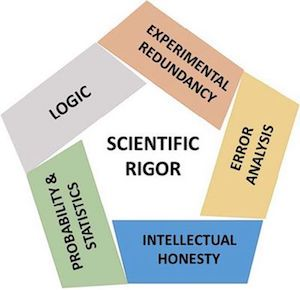
\includegraphics[width=0.99\linewidth]{images/F1_large} 

}

\caption{Rigorous Science according to @casadevall2016a.}\label{fig:rigorous}
\end{figure}

When a claim is based on \href{http://mbio.asm.org/content/7/6/e01902-16.full}{\textbf{Scientific Rigour}} \citep{casadevall2016a}, we mean it was posited based on the following set of principles:

\begin{enumerate}
\def\labelenumi{\arabic{enumi}.}
\tightlist
\item
  \textbf{Experimental Redundancy} - The claim has been examined by all methodological and analytical tools that are available and are appropriate given the context. Rigorous Science does not rely on one type of experimental design or one type of statistical analysis.
\item
  \textbf{Recognition of Error} - Without failure there can be no progress, therefore we should carefully study failures and not just report success stories. Any sources of error should be carefully studied and reported to the scientific community.
\item
  \textbf{Sound Probability \& Statistics} - Use of the most recent and appropriate statistical theories, models and analytical techniques. Statistical modelling techniques become more realistic over time and often the models that were taught in undergraduate statistics courses have long been replaced and should not be used any more.
\item
  \textbf{Efforts to Avoid Logical Traps} - When generating theories and defining constructs and laws, make sure logical inconsistencies are avoided. When making inferences, avoid the common logical traps such as \emph{The Effect = Structure Fallacy} in null hypothesis significance testing (NHST).
\item
  \textbf{Intellectual Honesty} - Rigorous science is ethical, has integrity and thrives on critical reflection on scientific practice. The right mindset is \emph{``Prove yourself wrong!''}, not \emph{``Prove yourself right!''}
\end{enumerate}

We add to the list that science must be open and transparent. This may seem like an obvious statement to a fresh student of human behaviour, but concepts that make up an essential part of the scientific debate in 2017, such as \emph{open science}, \emph{open data}, \emph{reproducibility}, \emph{Questionable Research Practices (QRPs)}, \emph{Hypothesizing After the Results are Known (HARKing)} and \emph{preregistration}, were practically unknown 5 years ago.

\hypertarget{theoretical-tunnelvision}{%
\subsection*{Theoretical Tunnelvision}\label{theoretical-tunnelvision}}
\addcontentsline{toc}{subsection}{Theoretical Tunnelvision}

\begin{quote}
``It is the theory that decides what we may observe''

---Einstein (as quoted by Heisenberg)
\end{quote}

Many of the initiatives proposed to improve the social and life sciences focus on improving methodology and statistics. This is understandable, it's where errors are easily made (and discovered) and it allows for relatively simple interventions, e.g.~more stringent control on appropriate use of statistics by journals. However, the goal of generating empirical facts is ultimately because we want to find out which scientific claim about the structure of reality best explains why those empirical facts were observed.

The quote attributed to Einstein refers to an important, and grossly underestimated phenomenon one might call the \emph{theoretical tunnelvision}. It is best explained by an example that is commonly encountered in the literature in psychological science and goes something like this:

\begin{enumerate}
\def\labelenumi{\arabic{enumi}.}
\tightlist
\item
  A study tries to find independent causes (predictors) of a certain disease-entity, a pathological state or behavioural mode people can `get stuck in'.
\item
  Typically, a statistical model fitted on a large, representative sample of individuals in which many different predictors were measured will yield associations between predictor and disease-entity that are significant but small (on average \(r \approx 0.3\), or \(\approx 9\%\) explained variance).
\item
  Often, if other known (non-clinical) covariates are included in a model, or, if the multivariate nature of the phenomenon is taken seriously by including repeated measurements and/or multiple dependent variables, these predictors will no longer explain any unique variance in the outcome measures.
\end{enumerate}

Here's an example of a `predictor' study \citep{walker2015a} to find predictors of persistence of Major Depressive Disorder MDD 10 over the course of 10 years in a representative sample of 331 individuals who suffered MDD 10 years earlier:

\begin{quote}
``Clinical variables in this analysis were not strongly associated with persistence of MDD over the course of 10 years. Comorbid generalized anxiety disorder, baseline depression severity, and taking a prescription for nerves, anxiety, or depression were significantly associated with persistent depression in the unadjusted logistic regression models, but the associations became non-significant when in the multivariate model. These findings are in contrast to the results from several other studies.''
\end{quote}

The study concludes by discussing three factors that play a statistically significant role in the persistence of MDD (text between brackets not in original):

\begin{itemize}
\tightlist
\item
  ``\emph{having two or more chronic medical conditions {[}in 1995-1996{]} contributes to experiencing depression ten years later.} {[}2.89 more likely{]} \emph{However, only having one chronic medical condition did not increase the odds of being classified as having MDD in 2004--2006.}''
\item
  ``\emph{days of activity limitation in 1995--1996 were significantly associated with a greater risk of depression ten years later,} {[}2.19 more likely{]} \emph{independent of the number of chronic medical conditions a person had.}''
\item
  ``\emph{Individuals who were in contact with family less than once a week} {[}in 1995-1996{]} \emph{were more likely to have MDD in 2004--2006.} {[}2.07 more likely{]} \emph{Likewise, people who were married were less likely to have persistent depression compared to those who have never married} {[}never married 2.42 more likely{]}''
\end{itemize}

\hypertarget{so-whats-wrong}{%
\subsection*{So? What's wrong?}\label{so-whats-wrong}}
\addcontentsline{toc}{subsection}{So? What's wrong?}

So what's wrong with these inferences? The study shows some previous assumptions about the relevance of clinical predictors should be reconsidered, and it adds to scientific record some facts about risk factors that might have eluded scientists, clinicians and health professionals. Let's look at the main conclusion of the study, in addition to a plea for more attention for people with two or more chronic medical conditions, \citet{walker2015a} end the article with:

\begin{quote}
Future research should continue to examine the complex nature of the relationship between chronic medical disorders and comorbid psychiatric conditions. Addressing these conditions and strengthening social support systems could be important strategies for reduce the burden of depression.
\end{quote}

Here's what is odd from the perspective of \emph{rigorous science}:

\begin{enumerate}
\def\labelenumi{\arabic{enumi}.}
\item
  If clinical predictors play no role in explaining why some people remain depressed for such long periods of time, why isn't the main conclusion of the study that we must re-appraise the scientific theories laying explanatory claim on the aetiology of MDD? It is from these theories that the diagnostic tools, the medical, and psychological interventions to which these patients have been exposed, were derived.
\item
  Even though the authors acknowledge --and indeed show-- that the propagation of a pathological state like MDD over many years is a very complex multivariate phenomenon, their suggestion for future research is still based on an implicit assumption about causation that is extremely simple. The idea is that there is a chain of unique (efficient) causes, each contributing independently to the emergence, and persistence in time of the MDD state. The authors basically suggest some component causes have to be added to the aetiology. The metaphor is that of a \emph{machine} of which the sum output of its constituent components is equal to the purpose or function of the machine as a whole. Should a component fail, then it can be repaired or replaced as long as it performs the same function as the defective part, thereby restoring the function of the machine as a whole. This is why the authors suggest that strengthening social support systems could be an intervention to reduce the burden of depression: The absence of a partner or visits by family members were predictors that explained some unique variance in the data on the persistence of MDD. Obviously, restoring this defective social support component should restore or at least facilitate the escape from the MDD state. Meanwhile, they seem to forget that they convincingly argued that MDD is a very complex phenomenon that cannot be dissected into neat, independent component causes.
\item
  Very much related to the previous point: The authors mention three important factors in the discussion and conclusion section, however, the results section contains another factor that was omitted, it is in fact the second most important predictor of the persistence of MDD:
\end{enumerate}

\begin{quote}
``Women had 2.48 the odds of remaining depressed compared to men''
\end{quote}

Why did they ignore this predictor in the discussion? This is speculation, but could it be that this factor is not mentioned because it would have to be considered a `deficient' component and suggesting any kind of `treatment' intended to `repair' it is of course beyond the realm of sane things to suggest. Nevertheless, it does seem rather important to figure out why women are 2.5 times more likely than men to still be depressed after 10 years. Perhaps \emph{not} considering gender to be a unique causal component in a chain of \emph{in}dependent predictors might help. Instead, gender could be considered a complex aggregate, or, contextual variable that is associated to the dependent variable through a vast network of \emph{inter}dependent facts, events and states of affair. An obvious factor of importance is that effect-studies of medical interventions are mainly conducted on white, male, 20-30 year old, right-handed, subjects with above average SES. Also, it is likely that on average, the stability of mood over longer periods of time is more variable in women than in men due to fluctuations of hormone levels, but also due to antenatal and postnatal depression \citep{world2002a}. It does not seem unreasonable to suggest this poses extra challenges for women who want to escape the MDD state.

\hypertarget{no-such-thing-as-theory-free-facts}{%
\subsection*{No such thing as theory-free `facts'}\label{no-such-thing-as-theory-free-facts}}
\addcontentsline{toc}{subsection}{No such thing as theory-free `facts'}

The analytical tools selected by the researchers (a generalized linear statistical model) restricts the kinds of associations we might observe in the data. In the the present case all associations will --after transformation-- be linear compositions of independent components.\footnote{Naturally, if one would use mixed models we can account for dependencies in the data, but they will still be limited to linear associations.} One never reads this valid equally valid conclusion: ``\emph{We conclude that the linear model is inadequate to describe the complexity of this phenomenon.}'' The reason is that the implicit assumptions about causality underlying scientific claims never enter the empirical cycle and therefore escape falsification by the repeated application of the scientific method even though those causality assumptions are also based on a scientific theory about the structure of reality that is in principle falsifiable.

To be a bit more precise about the relationship between what theories assume to be constituent parts of reality and why, we discuss the differences between some important theoretical concepts.

\hypertarget{phenomena-theories-facts-and-laws}{%
\section{\texorpdfstring{\textbf{Phenomena, theories, facts and laws}}{Phenomena, theories, facts and laws}}\label{phenomena-theories-facts-and-laws}}

\begin{quote}
``All science is either physics or stamp collecting.''

---Ernest Rutherford (Physics Nobel Laureate, 1872-1937)
\end{quote}

It's important to distinguish between phenomena, hypothesis, theory and law. For example, we will be discussing, \protect\hyperlink{Nonl49}{nonlinear \emph{phenomena}}, \protect\hyperlink{Cata9}{catastrophe \emph{theory}} and \protect\hyperlink{Powe58}{power \emph{law} scaling}.

The video is provides a very clear explanation of the differences between these concepts.

\BeginKnitrBlock{rmdimportant}
\href{https://youtu.be/lqk3TKuGNBA}{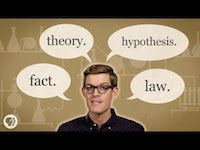
\includegraphics{images/facts.jpg}}
\EndKnitrBlock{rmdimportant}

\hypertarget{appraising-and-amending-theories}{%
\section{\texorpdfstring{\textbf{Appraising and amending theories}}{Appraising and amending theories}}\label{appraising-and-amending-theories}}

\begin{quote}
A difficulty of much psychological theorizing is vagueness in the terms employed. In this work, the above ideas have been studied in mathematical form throughout, the definitions and proofs being given corresponding precision.

---W. R. Ashby in `The Physical Origin of Adaptation by Trial adn Error' (\citeyearpar{ashby1945a}, p.~13)
\end{quote}

\hypertarget{strong-inference}{%
\subsection*{Strong Inference}\label{strong-inference}}
\addcontentsline{toc}{subsection}{Strong Inference}

\emph{The Effect = Structure Fallacy} refers to the logical error that occurs a predicted effect is observed (i.e.~a statistically significant test result leads to a rejection of the null hypothesis), it is not valid to infer the existence of the assumed cause was evidenced. NHST is based on \emph{the falsification principle}, which means the perceived veracity of a scientific claim will increase only if it has resisted many rigorous attempts to prove it is wrong. If a scientific claim has a large track-record of resisting falsification

\begin{table}[t]

\caption{\label{tab:stronInf}Strong Inference according to @platt1964strong }
\centering
\resizebox{\linewidth}{!}{
\fontsize{10}{12}\selectfont
\begin{tabular}{ll}
\toprule
  & Strong inference consists of applying the following steps to every problem in science, formally and explicitly and regularly:\\
\midrule
\rowcolor{gray!6}  1. & Devising alternative hypotheses\\
2. & Devising a crucial experiment (or several of them), with alternative possible outcomes, each of which will, as nearly as possible, exclude one or more of the hypotheses\\
\rowcolor{gray!6}  3. & Carrying out the experiment so as to get a clean result\\
1' & Recycling the procedure, making subhypotheses or sequential hypotheses to refine the possibilities that remain\\
\rowcolor{gray!6}  ... & and so on.\\
\bottomrule
\end{tabular}}
\end{table}

--\textgreater{}

--\textgreater{}
 --\textgreater{}
 --\textgreater{}
 --\textgreater{}
 --\textgreater{}
 --\textgreater{}
 --\textgreater{}
 --\textgreater{}
 --\textgreater{}

--\textgreater{}
 --\textgreater{}
 --\textgreater{}
 --\textgreater{}
 --\textgreater{}
 --\textgreater{}

--\textgreater{}
 --\textgreater{}
 --\textgreater{}
 --\textgreater{}
 --\textgreater{}

--\textgreater{}

--\textgreater{}
 --\textgreater{}
 --\textgreater{}
 --\textgreater{}
 --\textgreater{}
 --\textgreater{}
 --\textgreater{}
 --\textgreater{}
 --\textgreater{}
 --\textgreater{}

\hypertarget{study-materials}{%
\chapter*{\texorpdfstring{\emph{Study Materials}}{Study Materials}}\label{study-materials}}
\addcontentsline{toc}{chapter}{\emph{Study Materials}}

\BeginKnitrBlock{rmdimportant}
{Ontology.}

\href{https://youtu.be/FN2zwqE_Qo0}{
\includegraphics{images/epi_onto.jpg}}
\EndKnitrBlock{rmdimportant}

\BeginKnitrBlock{rmdimportant}
{Epistemology}

\href{https://youtu.be/jRxoHtGa4NM}{
\includegraphics{images/epis.jpg}}
\EndKnitrBlock{rmdimportant}

\hypertarget{introduction-to-complexity-science}{%
\chapter{\texorpdfstring{\textbf{Introduction to Complexity Science}}{Introduction to Complexity Science}}\label{introduction-to-complexity-science}}

Psychological systems are biological systems which are physical systems that are alive. Therefore, any theory that lays explanatory claim to phenomena of the mind, ultimately must be a theory about how a physical system is able to accumulate non-random order into its internal structure that appears to codetermine its behaviour. Less formally stated, a science that studies the behaviour of physical systems that are alive, that appear to have a memory which makes their behaviour adaptive, future oriented and intelligent, should be grounded in physical and biological principles and laws.

For now, that may be a bridge too far \citep[however, see][]{turvey2012a}, but current theories of human behaviour should at least not contradict highly corroborated theories of physics that also describe the behaviour of the constituent components of complex living systems.

\hypertarget{part-mathematics-of-change}{%
\part{Mathematics of Change}\label{part-mathematics-of-change}}

\hypertarget{introduction-to-the-mathematics-of-change}{%
\chapter{\texorpdfstring{\textbf{Introduction to the Mathematics of Change}}{Introduction to the Mathematics of Change}}\label{introduction-to-the-mathematics-of-change}}

The simplest non-trivial \emph{iterative change process} can be described by the following \emph{difference equation}:

\[ Y_{t+1} = Y_{t=0} + a*Y_t \]

The equation describes the way in which the value of \(Y\) changes \href{https://en.wikipedia.org/wiki/Discrete_time_and_continuous_time}{between two adjacent, \textbf{discrete} moments in time}
(hence the term \href{https://en.wikipedia.org/wiki/Recurrence_relation}{difference equation, or recurrence relation}). There are two parameters resembling an intercept and a slope:

\begin{enumerate}
\def\labelenumi{\arabic{enumi}.}
\tightlist
\item
  The starting value \(Y_0\) at \(t=0\), also called the \emph{starting value}, or the \emph{initial conditions}.
\item
  A rule for incrementing time, here the change in \(Y\) takes place over a discrete time step of 1: \(t+1\).
\end{enumerate}

The values taken on by variable \(Y\) are considered to represent the states quantifiable observable alternative ways to describe the change of states :

\begin{itemize}
\tightlist
\item
  A dynamical rule describing the propagation of the states of a system observable measured by the values of variable \texttt{Y} through discrete time.
\item
  A dynamic law describing the time-evolution of the states of a system observable measured by the variable \texttt{Y}.
\end{itemize}

These descriptions all refer to the change processes that govern system observables (properties of dynamical systems that can be observed through measurement).

\hypertarget{its-a-line-its-a-plane}{%
\section{\texorpdfstring{\textbf{It's a line! It's a plane!}}{It's a line! It's a plane!}}\label{its-a-line-its-a-plane}}

The formula resembles the equation of a line. There is a constant value \(Y_{0}\) which is added to a proportion of the value of \(Y\) at time \(t\), given by parameter \(a\). This is equivalent to the slope of a line. However, in a \((X,Y)\) plane there are two `spatial' (metric) dimensions representing the values two variables \(X\) and \(Y\) can take on (see figure).

\begin{center}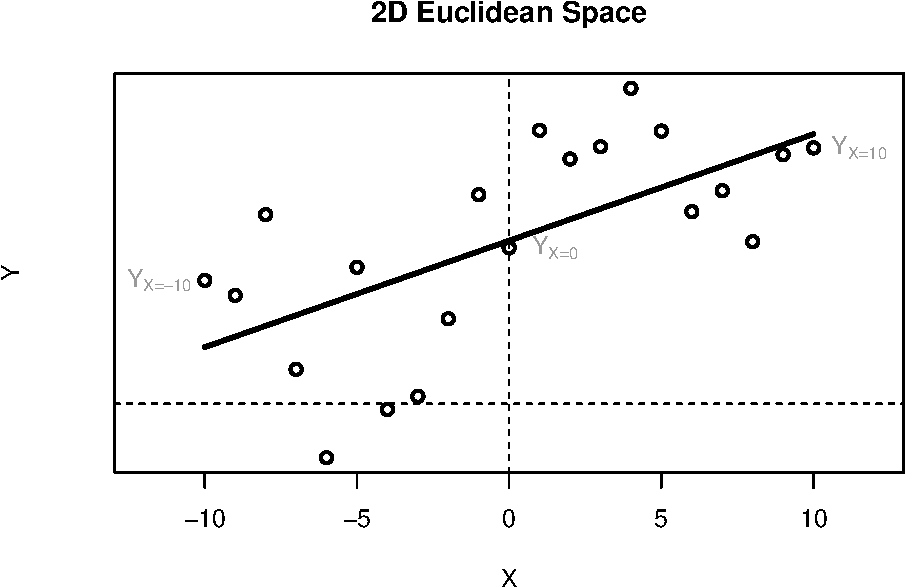
\includegraphics[width=0.99\linewidth]{CSA-Book_files/figure-latex/unnamed-chunk-2-1} \end{center}

The best fitting straight line would be called a statistical model of the linear relationship between the observed values of \(X\) and \(Y\). It can be obtained by fitting a General Linear Model (GLM) to the data. If \(X\) were to represent repeated measurements the multivariate GLM for repeated measures would have to be fitted to the data. This can be very problematic, because statistical models rely on \href{https://en.wikipedia.org/wiki/Ergodic_theory}{Ergodic theory}:

\begin{quote}
``\ldots{} it is the study of the long term average behavior of systems evolving in time.''
\end{quote}

\BeginKnitrBlock{rmdkennen}
In other words: If you throw 1 die 100 times in a row, the average of the 100 numbers is the \textbf{time-average} of one of the observables of die-throwing systems. If this system is ergodic, then its \textbf{time-average} is expected to be similar to the average of the numbers that turn up if you throw 100 dice all at the same instance of time. The dice layed out on the table represent a spatial sample, a snapshot frozen in time, of the possible states the system can be in. Taking the average would be the \textbf{spatial average} this observable of die-throwing systems. This ergodic condiciotn is often implicitly assumed in Behavioural Science when studies claim to study change by taking different samples of individuals (snapshots of system states) and comparing if they are the same.
\EndKnitrBlock{rmdkennen}

need to assume independence of measurements within and between subjects. These assumptions can be translated to certain conditions that must hold for the model to be valid, known as \emph{Compound Symmetry} and \emph{Sphericity}:

\begin{quote}
The compound symmetry assumption requires that the variances (pooled within-group) and covariances (across subjects) of the different repeated measures are homogeneous (identical). This is a sufficient condition for the univariate F test for repeated measures to be valid (i.e., for the reported F values to actually follow the F distribution). However, it is not a necessary condition. The sphericity assumption is a necessary and sufficient condition for the F test to be valid; it states that the within-subject ``model'' consists of independent (orthogonal) components. The nature of these assumptions, and the effects of violations are usually not well-described in ANOVA textbooks; \footnote{\href{https://www.statsoft.com/Textbook/ANOVA-MANOVA\#sphericity}{Retreived from www.statsoft.com}}
\end{quote}

As you can read in the quoted text above, these conditions must hold in order to be able to identify unique independent components as the sources of variation of \(Y\) over time within a subject. This is the a clear example of:

If you choose to use GLM repeated measures to model change over time, you will only be able to infer independent components that are responsible for the time-evolution of \(Y\). As is hinted in the last sentence of the quote, the validity of such inferences is not a common topic of discussion statistics textbooks.

\hypertarget{no-its-a-time-series}{%
\section{\texorpdfstring{\textbf{No! \ldots{} It's a time series!}}{No! \ldots{} It's a time series!}}\label{no-its-a-time-series}}

The important difference between a regular 2-dimensional Euclidean plane and the space in which we model change processes is that the \(X\)-axis represents the physical dimension \textbf{time}. In the case of the Linear Map we have a 1D space with one `spatial' dimension \(Y\) and a time dimension \(t\). This is called time series if \(Y\) is sampled as a continuous process, or a trial series if the time between subsequent observations is not relevant, just the fact that there was a temporal order (for example, a series of response latencies to trials in a psychological experiment in the order in which they were presented to the subject).

\begin{center}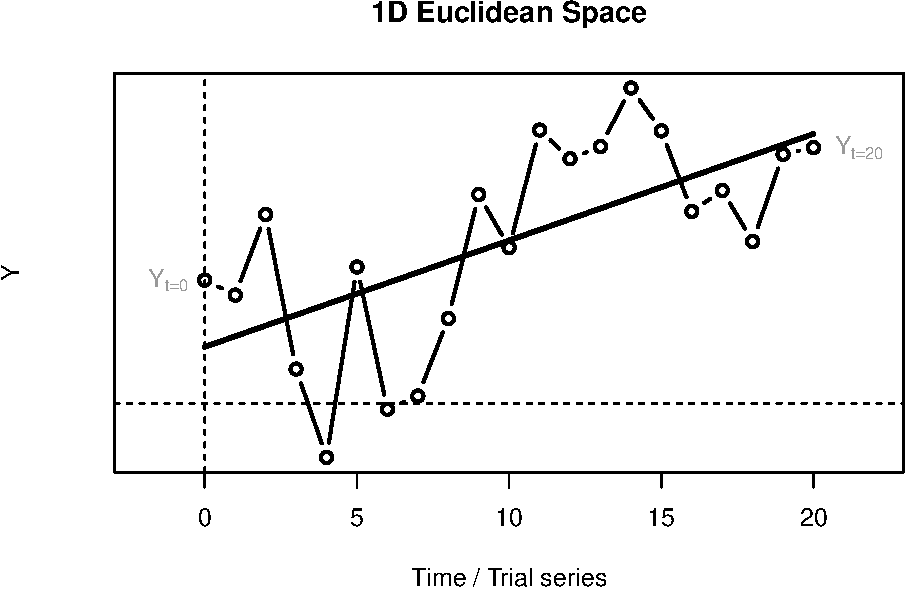
\includegraphics[width=0.99\linewidth]{CSA-Book_files/figure-latex/unnamed-chunk-4-1} \end{center}

Time behaves different from a spatial dimension in that it is directional (time cannot be reversed), it cannot take on negative values, and, unless one is dealing with a truly random process, there will be a temporal correlation across one or more values of \(Y\) separated by an amount of time. In the linear difference equation this occurs because each value one step in the future is calculated based on the current value. If the values of \(Y\) represent an observable of a dynamical system, the system can be said to have a history, or a memory.

Ergodic systems do \emph{not} have a history or a memory that extends across more than one time step. This is very convenient, because one can calculate the expected value of a system observable given infinite time, by making use of of the laws of probabilities of random events (or random fields). This means: The average of an observable of an Ergodic system measured across infinite time (its entire history, the \textbf{time-average}), will be the be the same value as the average of this observable measured at one instance in time, but in an infinite amount of systems of the same kind (the population, the \textbf{spatial average}) {[}\^{}dice{]}.

The simple linear difference equation will have a form of \emph{perfect memory} across the smallest time scale (i.e., the increment of 1, \(t+1\)). This `memory' just concerns a correlation of 1 between values at adjacent time points (a short range temporal correlation, SRC), because the change from \(Y_t\) to \(Y_{t+1}\) is exactly equal to \(a * Y_t\) at each iteration step. This is the meaning of deterministic, not that each value of \(Y\) is the same, but that the value of \(Y\) now can be perfectly explained form the value of \(Y\) one moment in the past.

Summarising, the most profound difference is not the fact that the equation of linear change is a deterministic model and the GLM is a probabilistic model with parameters fitted from data, this is something we can (and will) do for \(a\) as well. The profound difference between the models is the role given to the passage of time:

\begin{itemize}
\tightlist
\item
  The linear difference equation represents changes in \(Y\) as a function of the physical dimension \emph{time} and \(Y\) itself.
\item
  The GLM represents changes in \(Y\) as a function of a \href{https://en.wikipedia.org/wiki/Linear_predictor_function}{linear predictor} composed of additive components that can be regarded as independent sources of variation that sum up to the observed values of \(Y\).
\end{itemize}

\hypertarget{plotTS}{%
\section{\texorpdfstring{\textbf{\texttt{R}: The time series object}}{R: The time series object}}\label{plotTS}}

A time series object is expected to have a time-dimension on the x-axis. This is very convenient, because \texttt{R} will generate the time axis for you by looking at the \emph{t}ime \emph{s}eries \emph{p}roperties attribute of the object. Even though we are not working with measurement outcomes, consider a value at a time-index in a time series object a \textbf{sample}:

\begin{itemize}
\tightlist
\item
  \texttt{Start} - The value of time at the first sample in the series (e.g., \(0\), or \(1905\))
\item
  \texttt{End} - The value of time at the last sample in the series (e.g., \(100\), or \(2005\))
\item
  \texttt{Frequency} - The amount of time that passed between two samples, or, the sample rate (e.g., \(0.5\), or \(10\))
\end{itemize}

Examples of using the time series object.

\begin{Shaded}
\begin{Highlighting}[]
\KeywordTok{set.seed}\NormalTok{(}\DecValTok{2718282}\NormalTok{)}
\CommentTok{# Get a timeseries of 100 random numbers }
\NormalTok{Y <-}\StringTok{ }\KeywordTok{ts}\NormalTok{(}\KeywordTok{rnorm}\NormalTok{(}\DecValTok{100}\NormalTok{))}
\CommentTok{# plot.ts}
\KeywordTok{plot}\NormalTok{(Y)}
\end{Highlighting}
\end{Shaded}

\begin{center}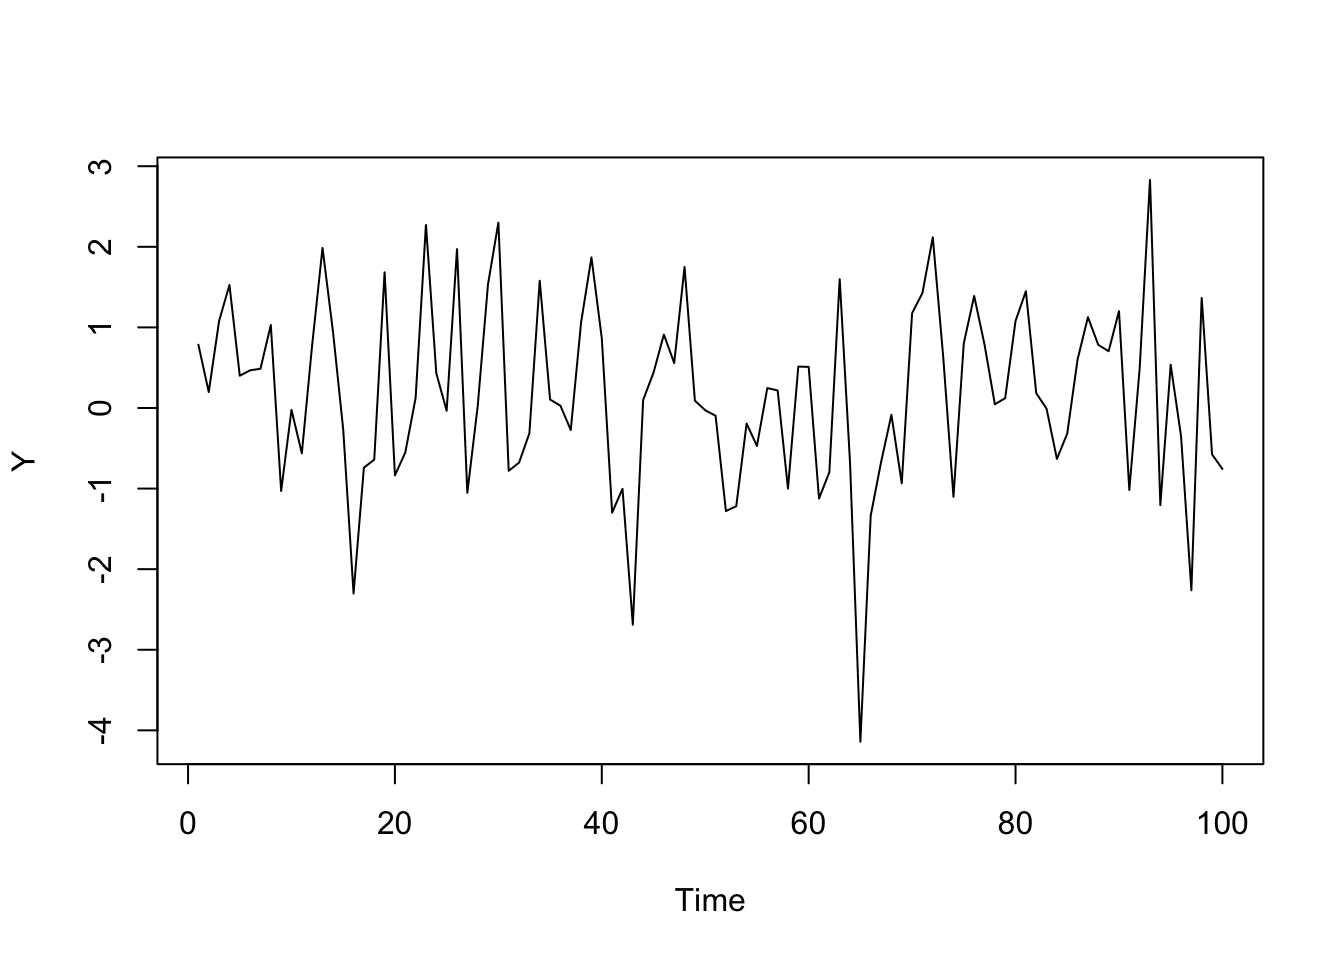
\includegraphics[width=0.99\linewidth]{CSA-Book_files/figure-latex/unnamed-chunk-5-1} \end{center}

\begin{Shaded}
\begin{Highlighting}[]
\CommentTok{# Get sample rate info}
\KeywordTok{tsp}\NormalTok{(Y)}
\end{Highlighting}
\end{Shaded}

\begin{verbatim}
## [1]   1 100   1
\end{verbatim}

\begin{Shaded}
\begin{Highlighting}[]
\CommentTok{# Extract the time vector}
\KeywordTok{time}\NormalTok{(Y)}
\end{Highlighting}
\end{Shaded}

\begin{verbatim}
## Time Series:
## Start = 1 
## End = 100 
## Frequency = 1 
##   [1]   1   2   3   4   5   6   7   8   9  10  11  12  13  14  15  16  17
##  [18]  18  19  20  21  22  23  24  25  26  27  28  29  30  31  32  33  34
##  [35]  35  36  37  38  39  40  41  42  43  44  45  46  47  48  49  50  51
##  [52]  52  53  54  55  56  57  58  59  60  61  62  63  64  65  66  67  68
##  [69]  69  70  71  72  73  74  75  76  77  78  79  80  81  82  83  84  85
##  [86]  86  87  88  89  90  91  92  93  94  95  96  97  98  99 100
\end{verbatim}

For now, these values are in principle all arbitrary units (\texttt{a.u.}). These settings only make sense if they represent the parameters of an actual measurement procedure.

It is easy to adjust the time vector, by assigning new values using \texttt{tsp()} (values have to be possible given the time series length). For example, suppose the sampling frequency was \(0.1\) instead of \(1\) and the Start time was \(10\) and End time was \(1000\).

\begin{Shaded}
\begin{Highlighting}[]
\CommentTok{# Assign new values}
\NormalTok{(}\KeywordTok{tsp}\NormalTok{(Y) <-}\StringTok{ }\KeywordTok{c}\NormalTok{(}\DecValTok{10}\NormalTok{, }\DecValTok{1000}\NormalTok{, }\FloatTok{.1}\NormalTok{))}
\end{Highlighting}
\end{Shaded}

\begin{verbatim}
## [1] 1e+01 1e+03 1e-01
\end{verbatim}

\begin{Shaded}
\begin{Highlighting}[]
\CommentTok{# Time axis is automatically adjusted }
\KeywordTok{time}\NormalTok{(Y)}
\end{Highlighting}
\end{Shaded}

\begin{verbatim}
## Time Series:
## Start = 10 
## End = 1000 
## Frequency = 0.1 
##   [1]   10   20   30   40   50   60   70   80   90  100  110  120  130  140
##  [15]  150  160  170  180  190  200  210  220  230  240  250  260  270  280
##  [29]  290  300  310  320  330  340  350  360  370  380  390  400  410  420
##  [43]  430  440  450  460  470  480  490  500  510  520  530  540  550  560
##  [57]  570  580  590  600  610  620  630  640  650  660  670  680  690  700
##  [71]  710  720  730  740  750  760  770  780  790  800  810  820  830  840
##  [85]  850  860  870  880  890  900  910  920  930  940  950  960  970  980
##  [99]  990 1000
\end{verbatim}

\hypertarget{plotting-a-ts-object-as-a-time-series}{%
\subsection{\texorpdfstring{Plotting a \texttt{ts} object as a time series}{Plotting a ts object as a time series}}\label{plotting-a-ts-object-as-a-time-series}}

Depending on which packages you use, there will be different settings applied to time series objects created by \texttt{ts()}. Below are some examples of differences between plotting routines.

\begin{Shaded}
\begin{Highlighting}[]
\KeywordTok{require}\NormalTok{(lattice)       }\CommentTok{# Needed for plotting}
\KeywordTok{require}\NormalTok{(latticeExtra)  }\CommentTok{# Needed for plotting}
\KeywordTok{require}\NormalTok{(casnet)        }\CommentTok{# Need for ts_center()}

\CommentTok{# stats::plot.ts}
\KeywordTok{plot}\NormalTok{(Y, }\DataTypeTok{lwd =} \DecValTok{2}\NormalTok{, }\DataTypeTok{main =} \StringTok{"stats::plot.ts"}\NormalTok{)}
\end{Highlighting}
\end{Shaded}

\begin{center}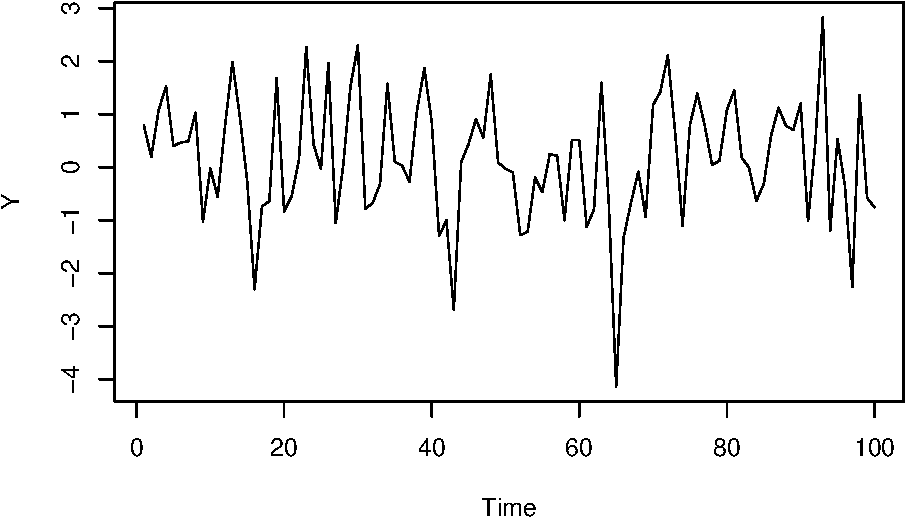
\includegraphics[width=0.99\linewidth]{CSA-Book_files/figure-latex/unnamed-chunk-7-1} \end{center}

\begin{Shaded}
\begin{Highlighting}[]
\CommentTok{# lattice::xyplot.ts}
\KeywordTok{xyplot}\NormalTok{(Y, }\DataTypeTok{lwd =} \DecValTok{2}\NormalTok{, }\DataTypeTok{main =} \StringTok{"lattice::xyplot.ts"}\NormalTok{)}
\end{Highlighting}
\end{Shaded}

\begin{center}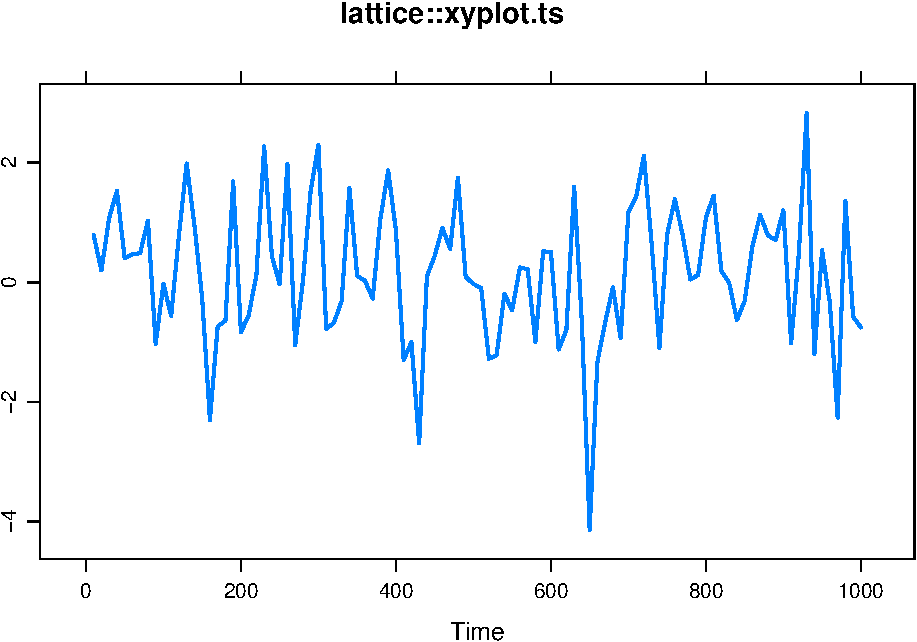
\includegraphics[width=0.99\linewidth]{CSA-Book_files/figure-latex/unnamed-chunk-7-2} \end{center}

\hypertarget{plotting-multiple-time-series-in-one-figure}{%
\subsection{Plotting multiple time series in one figure}\label{plotting-multiple-time-series-in-one-figure}}

Plot multiple time series in frames with \texttt{plot.ts()} in \texttt{package::stats}.
This function takes a matrix as input, here we use \texttt{cbind(\ ...\ )}.

\begin{Shaded}
\begin{Highlighting}[]
\CommentTok{# stats::plot.ts  }
\KeywordTok{plot}\NormalTok{(}\KeywordTok{cbind}\NormalTok{(Y,}
           \KeywordTok{cumsum}\NormalTok{(Y), }
           \KeywordTok{cumsum}\NormalTok{(}\KeywordTok{ts_center}\NormalTok{(Y))}
\NormalTok{           ), }
     \DataTypeTok{yax.flip =} \OtherTok{TRUE}\NormalTok{, }\DataTypeTok{col =} \StringTok{"blue"}\NormalTok{, }\DataTypeTok{frame.plot =} \OtherTok{TRUE}\NormalTok{, }
     \DataTypeTok{main =} \KeywordTok{expression}\NormalTok{(}\KeywordTok{paste}\NormalTok{(}\StringTok{"Random Numbers: "}\NormalTok{,}\KeywordTok{N}\NormalTok{(}\DecValTok{0}\NormalTok{,sigma))), }\DataTypeTok{xlab =} \StringTok{"time (a.u.)"}\NormalTok{)}
\end{Highlighting}
\end{Shaded}

\begin{center}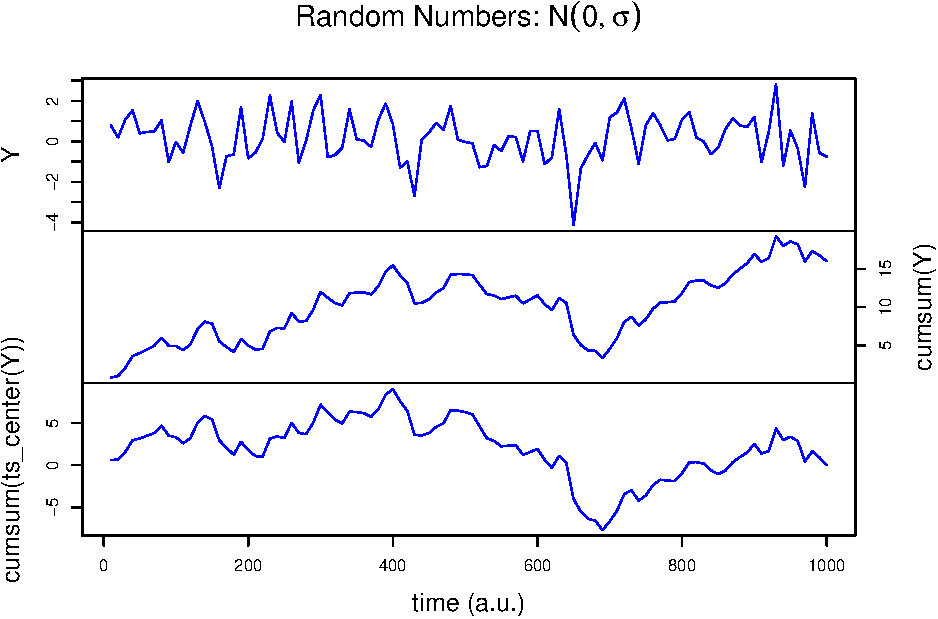
\includegraphics[width=0.99\linewidth]{CSA-Book_files/figure-latex/unnamed-chunk-8-1} \end{center}

Plot multiple time series in one graph with \texttt{ts.plot()} in \texttt{package::graphics}.
This function can handle multiple \texttt{ts} objects as arguments.

\begin{Shaded}
\begin{Highlighting}[]
\CommentTok{# graphics::ts.plot}
\KeywordTok{ts.plot}\NormalTok{(Y,}
        \KeywordTok{cumsum}\NormalTok{(Y), }
        \KeywordTok{cumsum}\NormalTok{(}\KeywordTok{ts_center}\NormalTok{(Y)),}
        \DataTypeTok{gpars =} \KeywordTok{list}\NormalTok{(}\DataTypeTok{xlab =} \StringTok{"time (a.u.)"}\NormalTok{,}
                     \DataTypeTok{ylab =} \KeywordTok{expression}\NormalTok{(}\KeywordTok{Y}\NormalTok{(t)),}
                     \DataTypeTok{main =} \KeywordTok{expression}\NormalTok{(}\KeywordTok{paste}\NormalTok{(}\StringTok{"Random Numbers: "}\NormalTok{,}\KeywordTok{N}\NormalTok{(}\DecValTok{0}\NormalTok{,sigma))),}
                     \DataTypeTok{lwd =} \KeywordTok{rep}\NormalTok{(}\DecValTok{2}\NormalTok{,}\DecValTok{3}\NormalTok{),}
                     \DataTypeTok{lty =} \KeywordTok{c}\NormalTok{(}\DecValTok{1}\OperatorTok{:}\DecValTok{3}\NormalTok{),}
                     \DataTypeTok{col =} \KeywordTok{c}\NormalTok{(}\StringTok{"darkred"}\NormalTok{,}\StringTok{"darkblue"}\NormalTok{,}\StringTok{"darkgreen"}\NormalTok{)}
\NormalTok{                     )}
\NormalTok{        )}
\KeywordTok{legend}\NormalTok{(}\DecValTok{0}\NormalTok{, }\DecValTok{18}\NormalTok{, }\KeywordTok{c}\NormalTok{(}\StringTok{"Y"}\NormalTok{,}\StringTok{"cumsum(Y)"}\NormalTok{, }\StringTok{"cumsum(ts_center(Y))"}\NormalTok{), }\DataTypeTok{lwd =} \KeywordTok{rep}\NormalTok{(}\DecValTok{2}\NormalTok{,}\DecValTok{3}\NormalTok{), }\DataTypeTok{lty =} \KeywordTok{c}\NormalTok{(}\DecValTok{1}\OperatorTok{:}\DecValTok{3}\NormalTok{), }\DataTypeTok{col =} \KeywordTok{c}\NormalTok{(}\StringTok{"darkred"}\NormalTok{,}\StringTok{"darkblue"}\NormalTok{,}\StringTok{"darkgreen"}\NormalTok{), }\DataTypeTok{merge =} \OtherTok{TRUE}\NormalTok{, }\DataTypeTok{cex=}\NormalTok{.}\DecValTok{9}\NormalTok{)}
\end{Highlighting}
\end{Shaded}

\begin{center}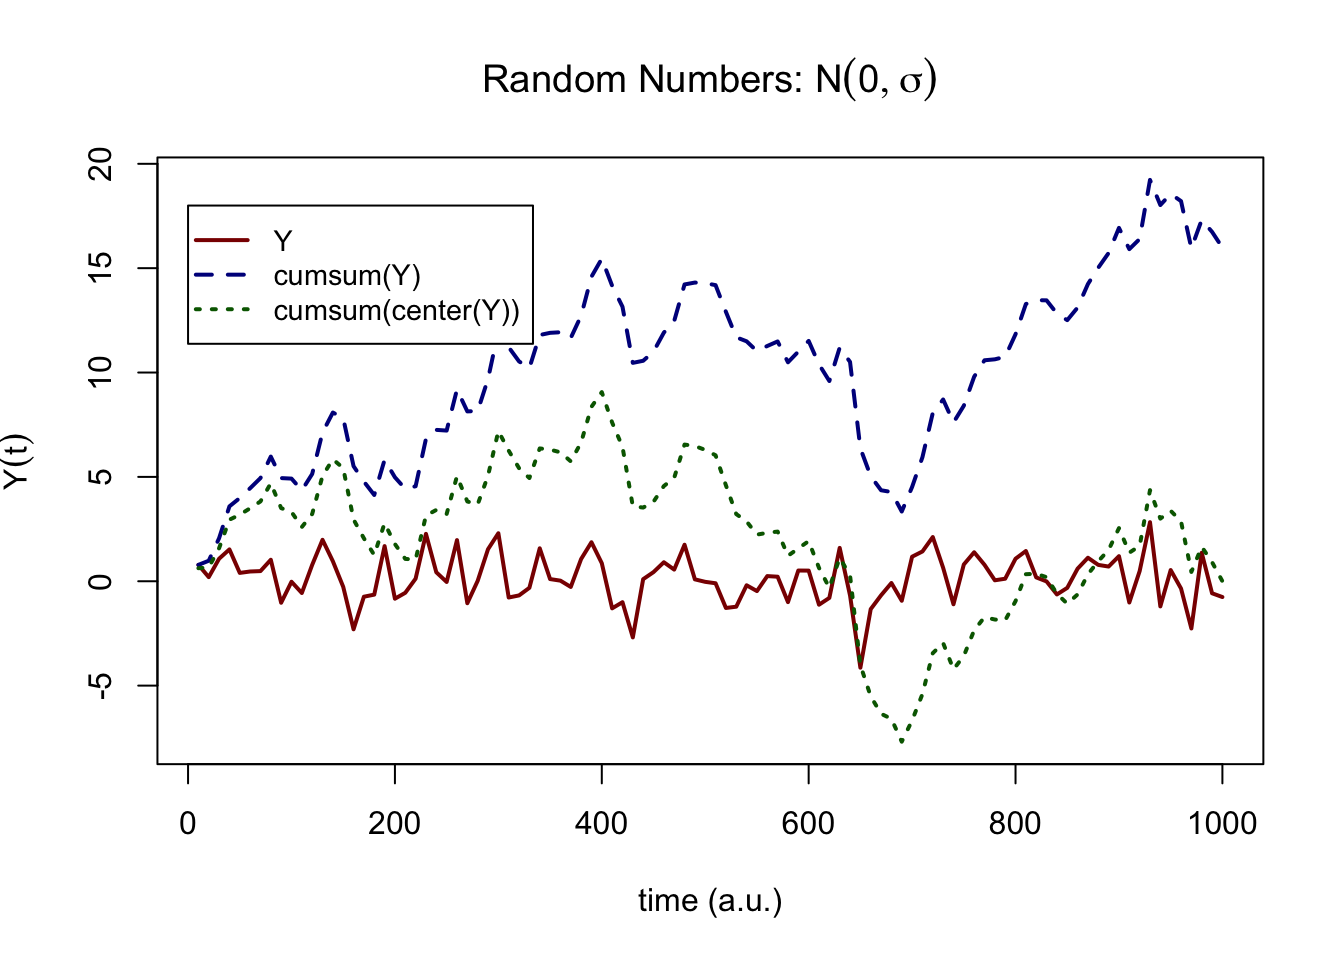
\includegraphics[width=0.99\linewidth]{CSA-Book_files/figure-latex/unnamed-chunk-9-1} \end{center}

Use \texttt{xyplot()} in \texttt{package::lattice} to create a plot with panels. The easiest way to do this is to create a dataset in so-called ``long'' format. This means the variable to plot is in 1 column and other variables indicate different levels, or conditions under which the variable was observed or simulated.

Function \texttt{ldply()} is used to generate \(Y\) for three different settings of \(r\). The values of \(r\) are passed as a \textbf{l}ist and after a function is applied the result is returned as a \textbf{d}ataframe.

\begin{Shaded}
\begin{Highlighting}[]
\KeywordTok{require}\NormalTok{(plyr)          }\CommentTok{# Needed for function ldply()}

\CommentTok{# Create a long format dataframe for various values for `r`}
\NormalTok{data <-}\StringTok{ }\KeywordTok{cbind.data.frame}\NormalTok{(}\DataTypeTok{Y     =} \KeywordTok{c}\NormalTok{(}\KeywordTok{as.numeric}\NormalTok{(Y), }\KeywordTok{cumsum}\NormalTok{(Y), }\KeywordTok{cumsum}\NormalTok{(}\KeywordTok{ts_center}\NormalTok{(Y))),}
                         \DataTypeTok{time  =} \KeywordTok{c}\NormalTok{(}\KeywordTok{time}\NormalTok{(Y), }\KeywordTok{time}\NormalTok{(Y), }\KeywordTok{time}\NormalTok{(Y)),}
                         \DataTypeTok{label =} \KeywordTok{factor}\NormalTok{(}\KeywordTok{c}\NormalTok{(}\KeywordTok{rep}\NormalTok{(}\StringTok{"Y"}\NormalTok{,}\KeywordTok{length}\NormalTok{(Y)),  }\KeywordTok{rep}\NormalTok{(}\StringTok{"cumsum(Y)"}\NormalTok{,}\KeywordTok{length}\NormalTok{(Y)), }\KeywordTok{rep}\NormalTok{(}\StringTok{"cumsum(ts_center(Y))"}\NormalTok{,}\KeywordTok{length}\NormalTok{(Y))))}
\NormalTok{                         )}
\CommentTok{# Plot using the formula interface}
\KeywordTok{xyplot}\NormalTok{(Y }\OperatorTok{~}\StringTok{ }\NormalTok{time }\OperatorTok{|}\StringTok{ }\NormalTok{label, }\DataTypeTok{data =}\NormalTok{ data, }\DataTypeTok{type =} \StringTok{"l"}\NormalTok{, }\DataTypeTok{main =} \KeywordTok{expression}\NormalTok{(}\KeywordTok{paste}\NormalTok{(}\StringTok{"Random Numbers: "}\NormalTok{,}\KeywordTok{N}\NormalTok{(}\DecValTok{0}\NormalTok{,sigma))))}
\end{Highlighting}
\end{Shaded}

\begin{center}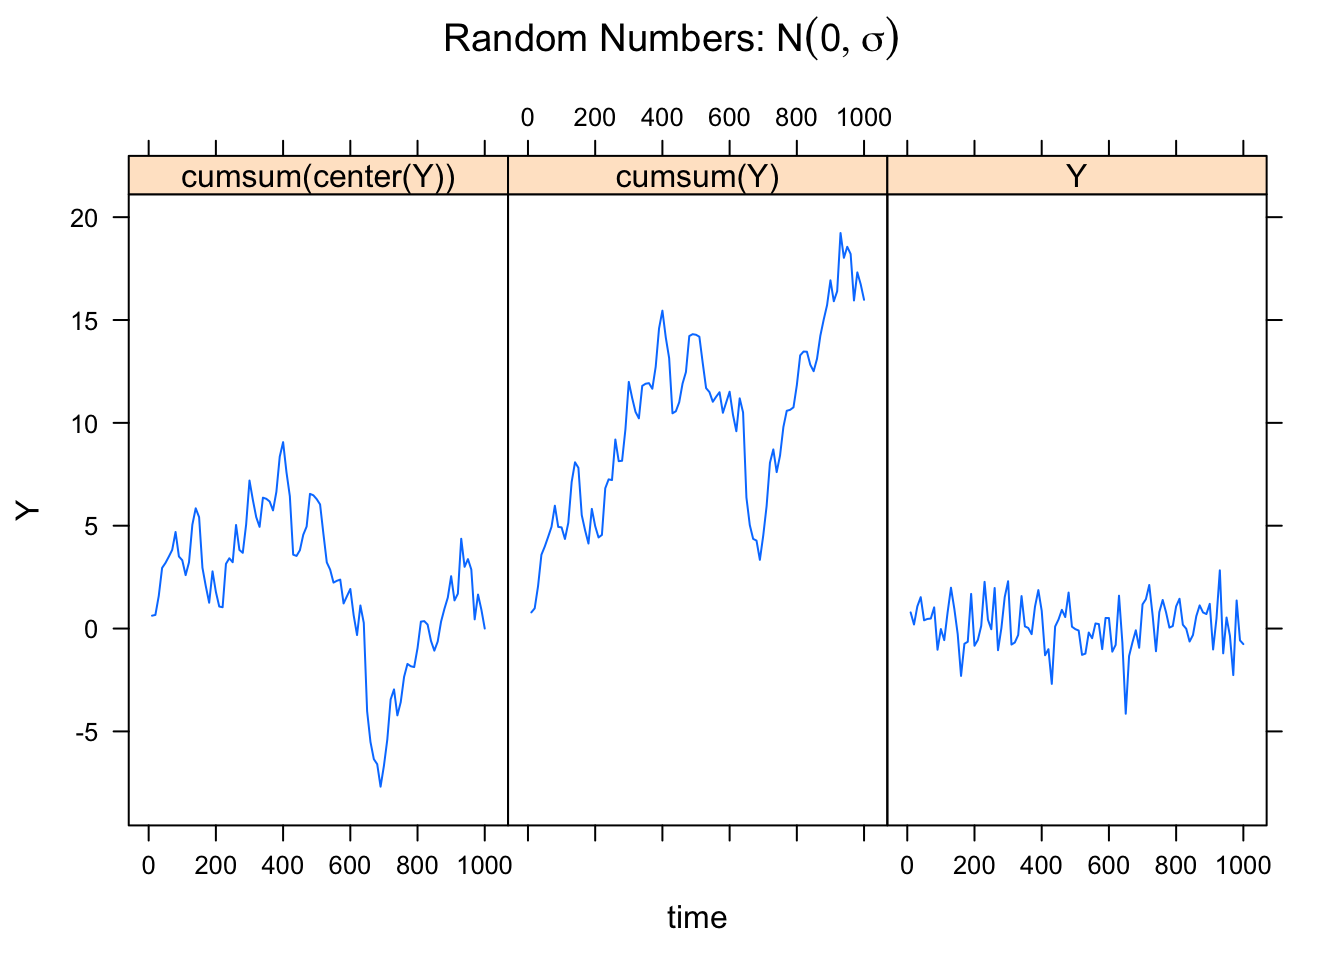
\includegraphics[width=0.99\linewidth]{CSA-Book_files/figure-latex/unnamed-chunk-10-1} \end{center}

\hypertarget{the-return-plot}{%
\subsection{The return plot}\label{the-return-plot}}

To create a return plot the values of \(Y\) have to be shifted by a certain lag. The functions \texttt{lead()} and \texttt{lag()} in \texttt{package::dplyr} are excellent for this purpose (note that \texttt{dplyr::lag()} behaves different from \texttt{stats::lag()}).

\begin{Shaded}
\begin{Highlighting}[]
\CommentTok{# Function lag() and lead()}
\KeywordTok{library}\NormalTok{(dplyr)}
\KeywordTok{library}\NormalTok{(casnet)}

\CommentTok{# Get exponential growth}
\NormalTok{YY <-}\StringTok{ }\KeywordTok{growth_ac}\NormalTok{(}\DataTypeTok{N=}\DecValTok{1000}\NormalTok{,}\DataTypeTok{r=}\FloatTok{1.5}\NormalTok{,}\DataTypeTok{type =} \StringTok{"driving"}\NormalTok{)}
\NormalTok{Y1 <-}\StringTok{ }\KeywordTok{as.numeric}\NormalTok{(YY}\OperatorTok{/}\KeywordTok{max}\NormalTok{(YY))}
\CommentTok{# Get logistic growth in the chaotic regime}
\NormalTok{Y2 <-}\StringTok{ }\KeywordTok{as.numeric}\NormalTok{(}\KeywordTok{growth_ac}\NormalTok{(}\DataTypeTok{N=}\DecValTok{1000}\NormalTok{,}\DataTypeTok{r=}\DecValTok{4}\NormalTok{,}\DataTypeTok{type =} \StringTok{"logistic"}\NormalTok{))}
\CommentTok{# Use the `lag` function from package `dplyr`}
\NormalTok{op <-}\StringTok{ }\KeywordTok{par}\NormalTok{(}\DataTypeTok{mfrow =} \KeywordTok{c}\NormalTok{(}\DecValTok{1}\NormalTok{,}\DecValTok{2}\NormalTok{), }\DataTypeTok{pty =} \StringTok{"s"}\NormalTok{)}
\KeywordTok{plot}\NormalTok{(dplyr}\OperatorTok{::}\KeywordTok{lag}\NormalTok{(Y1), Y1, }\DataTypeTok{xy.labels =} \OtherTok{FALSE}\NormalTok{, }\DataTypeTok{pch =} \DecValTok{16}\NormalTok{, }\DataTypeTok{xlim =} \KeywordTok{c}\NormalTok{(}\DecValTok{0}\NormalTok{,}\DecValTok{1}\NormalTok{), }\DataTypeTok{ylim =} \KeywordTok{c}\NormalTok{(}\DecValTok{0}\NormalTok{,}\DecValTok{1}\NormalTok{), }\DataTypeTok{xlab =} \StringTok{"Y(t)"}\NormalTok{, }\DataTypeTok{ylab =} \StringTok{"Y(t+1)"}\NormalTok{,}
     \DataTypeTok{main =} \StringTok{"exponential / max"}\NormalTok{)}
\KeywordTok{plot}\NormalTok{(dplyr}\OperatorTok{::}\KeywordTok{lag}\NormalTok{(Y2), Y2, }\DataTypeTok{xy.labels =} \OtherTok{FALSE}\NormalTok{, }\DataTypeTok{pch =} \DecValTok{16}\NormalTok{, }\DataTypeTok{xlim =} \KeywordTok{c}\NormalTok{(}\DecValTok{0}\NormalTok{,}\DecValTok{1}\NormalTok{), }\DataTypeTok{ylim =} \KeywordTok{c}\NormalTok{(}\DecValTok{0}\NormalTok{,}\DecValTok{1}\NormalTok{), }\DataTypeTok{xlab =} \StringTok{"Y(t)"}\NormalTok{, }\DataTypeTok{ylab =} \StringTok{"Y(t+1)"}\NormalTok{,}
     \DataTypeTok{main =} \StringTok{"logistic / max"}\NormalTok{)}
\end{Highlighting}
\end{Shaded}

\begin{center}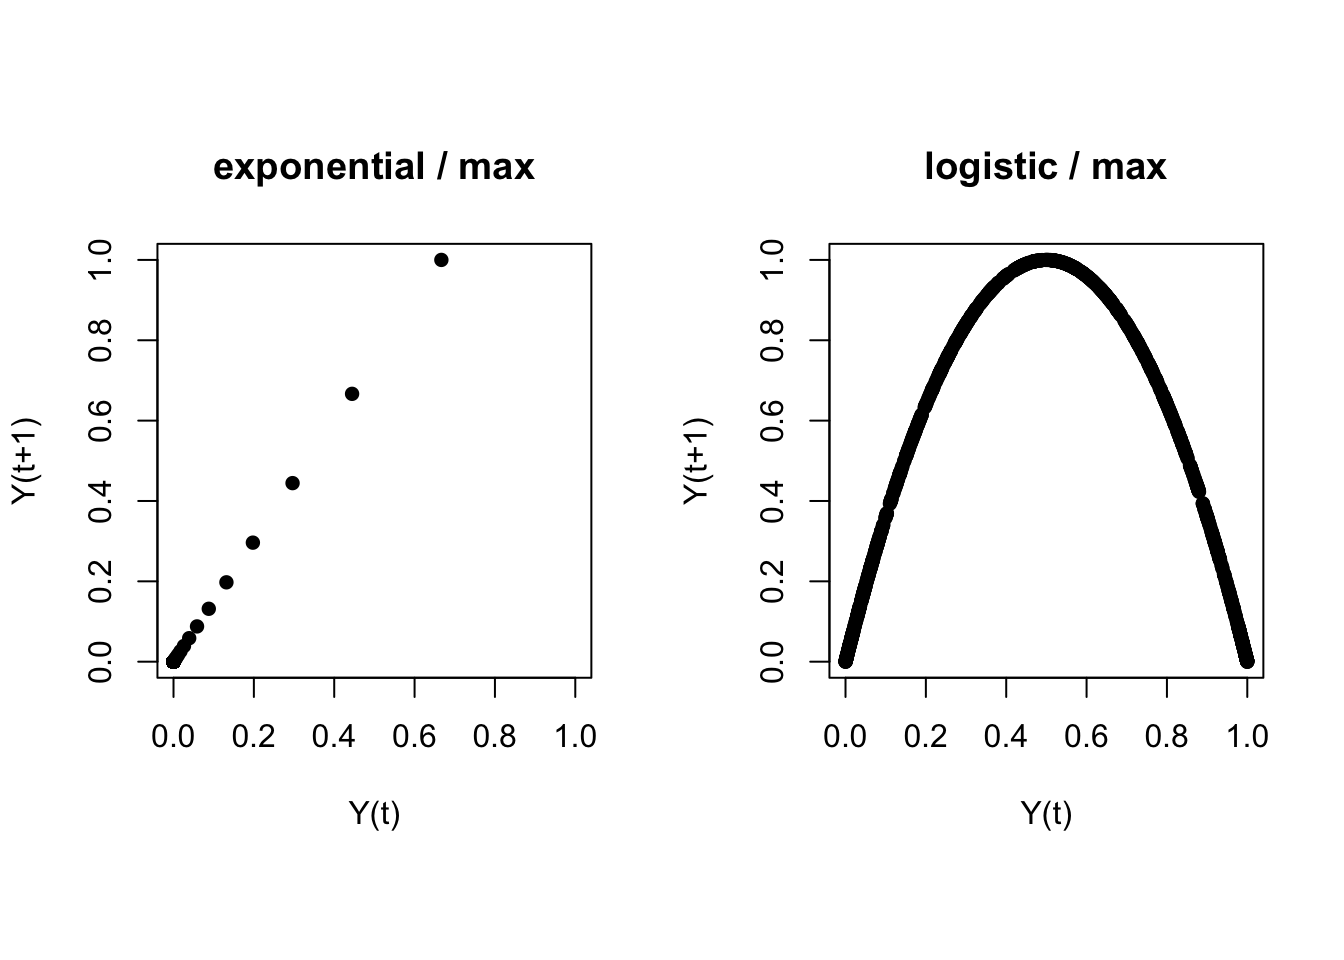
\includegraphics[width=0.99\linewidth]{CSA-Book_files/figure-latex/unnamed-chunk-11-1} \end{center}

\begin{Shaded}
\begin{Highlighting}[]
\KeywordTok{par}\NormalTok{(op)}
\end{Highlighting}
\end{Shaded}

Use \texttt{l\_ply()} from \texttt{package::plyr} to create return plots with different lags. The \textbf{l\_} before \textbf{ply} means the function will take a \textbf{l}ist as input to a function, but it will not expect any data to be returned, for example in the case of a function that is used to plot something.

\begin{Shaded}
\begin{Highlighting}[]
\CommentTok{# Explore different lags}
\NormalTok{op <-}\StringTok{ }\KeywordTok{par}\NormalTok{(}\DataTypeTok{mfrow =} \KeywordTok{c}\NormalTok{(}\DecValTok{1}\NormalTok{,}\DecValTok{2}\NormalTok{), }\DataTypeTok{pty =} \StringTok{"s"}\NormalTok{)}
\NormalTok{plyr}\OperatorTok{::}\KeywordTok{l_ply}\NormalTok{(}\DecValTok{1}\OperatorTok{:}\DecValTok{4}\NormalTok{, }\ControlFlowTok{function}\NormalTok{(l) }\KeywordTok{plot}\NormalTok{(dplyr}\OperatorTok{::}\KeywordTok{lag}\NormalTok{(Y2, }\DataTypeTok{n =}\NormalTok{ l), Y2, }\DataTypeTok{xy.labels =} \OtherTok{FALSE}\NormalTok{, }\DataTypeTok{pch =} \DecValTok{16}\NormalTok{, }\DataTypeTok{xlim =} \KeywordTok{c}\NormalTok{(}\DecValTok{0}\NormalTok{,}\DecValTok{1}\NormalTok{), }\DataTypeTok{ylim =} \KeywordTok{c}\NormalTok{(}\DecValTok{0}\NormalTok{,}\DecValTok{1}\NormalTok{), }\DataTypeTok{xlab =} \StringTok{"Y(t)"}\NormalTok{, }\DataTypeTok{ylab =} \KeywordTok{paste0}\NormalTok{(}\StringTok{"Y(t+"}\NormalTok{,l,}\StringTok{")"}\NormalTok{), }\DataTypeTok{cex =} \FloatTok{.8}\NormalTok{))}
\end{Highlighting}
\end{Shaded}

\begin{center}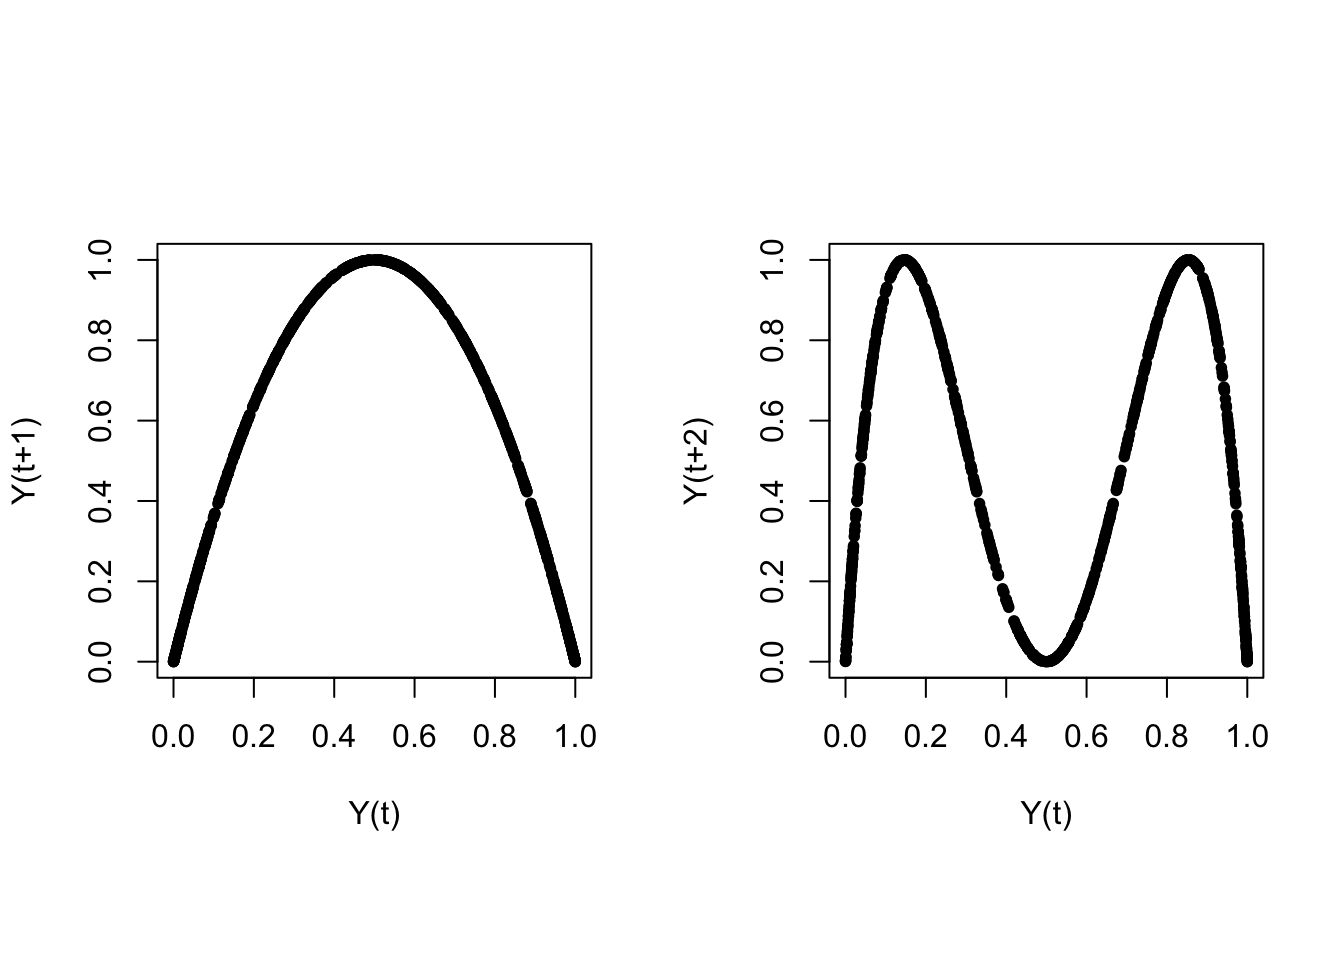
\includegraphics[width=0.99\linewidth]{CSA-Book_files/figure-latex/unnamed-chunk-12-1} \end{center}

\begin{center}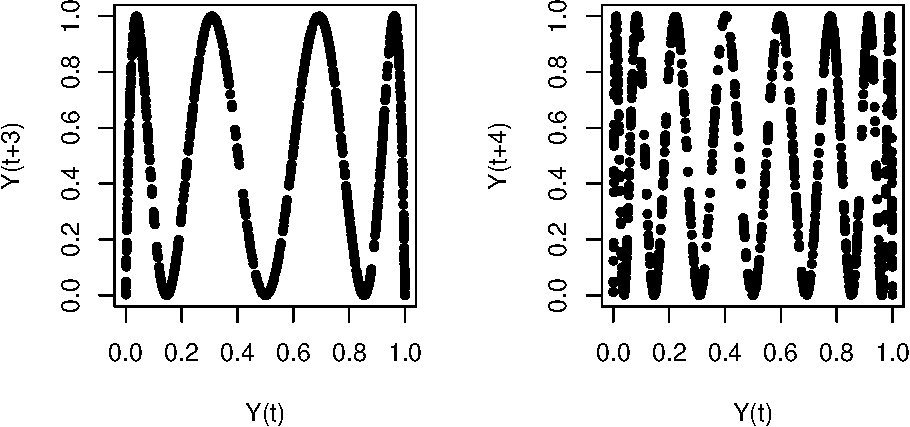
\includegraphics[width=0.99\linewidth]{CSA-Book_files/figure-latex/unnamed-chunk-12-2} \end{center}

\begin{Shaded}
\begin{Highlighting}[]
\KeywordTok{par}\NormalTok{(op)}
\end{Highlighting}
\end{Shaded}

\hypertarget{using-ggplot2}{%
\subsection{\texorpdfstring{Using \texttt{ggplot2}}{Using ggplot2}}\label{using-ggplot2}}

Becoming proficient at \texttt{ggplot2} can take some time, but it does pay off. One of the problems with plotting time series data is that \texttt{ggplot2} wants tidy data in \emph{long} format. Tidy data is:

\begin{quote}
Tidy data is a standard way of mapping the meaning of a dataset to its structure. A dataset is
messy or tidy depending on how rows, columns and tables are matched up with observations,
variables and types. In tidy data:
1. Each variable forms a column.
2. Each observation forms a row.
3. Each type of observational unit forms a table.

---\citet{wickham2014a}
\end{quote}

So if we have a set of time series as in the previous examples, we need to change it to long format.

\begin{Shaded}
\begin{Highlighting}[]
\KeywordTok{library}\NormalTok{(tidyverse)}

\CommentTok{# A wide data frame}
\NormalTok{df.wide <-}\StringTok{ }\KeywordTok{data.frame}\NormalTok{(}\DataTypeTok{rnormY        =}\NormalTok{ Y,}
                      \DataTypeTok{cumsumY       =} \KeywordTok{cumsum}\NormalTok{(Y), }
                      \DataTypeTok{centercumsumY =} \KeywordTok{cumsum}\NormalTok{(}\KeywordTok{ts_center}\NormalTok{(Y)),}
                      \DataTypeTok{time          =} \KeywordTok{seq_along}\NormalTok{(Y)}
\NormalTok{                      )}

\KeywordTok{glimpse}\NormalTok{(df.wide)}
\end{Highlighting}
\end{Shaded}

\begin{verbatim}
## Observations: 100
## Variables: 4
## $ rnormY        <dbl> 0.78482166, 0.19776074, 1.07957851, 1.52605836, ...
## $ cumsumY       <dbl> 0.7848217, 0.9825824, 2.0621609, 3.5882193, 3.98...
## $ centercumsumY <dbl> 0.6249966, 0.6629322, 1.5826857, 2.9489189, 3.18...
## $ time          <int> 1, 2, 3, 4, 5, 6, 7, 8, 9, 10, 11, 12, 13, 14, 1...
\end{verbatim}

\begin{Shaded}
\begin{Highlighting}[]
\CommentTok{# Create a long dataframe using gather()}
\NormalTok{df.long <-}\StringTok{ }\NormalTok{df.wide }\OperatorTok\StringTok{ }
\StringTok{  }\KeywordTok{gather}\NormalTok{(}\DataTypeTok{key=}\NormalTok{TimeSeries,}\DataTypeTok{value=}\NormalTok{Y,}\OperatorTok{-}\StringTok{"time"}\NormalTok{)}

\KeywordTok{glimpse}\NormalTok{(df.long)}
\end{Highlighting}
\end{Shaded}

\begin{verbatim}
## Observations: 300
## Variables: 3
## $ time       <int> 1, 2, 3, 4, 5, 6, 7, 8, 9, 10, 11, 12, 13, 14, 15, ...
## $ TimeSeries <chr> "rnormY", "rnormY", "rnormY", "rnormY", "rnormY", "...
## $ Y          <dbl> 0.78482166, 0.19776074, 1.07957851, 1.52605836, 0.4...
\end{verbatim}

\begin{Shaded}
\begin{Highlighting}[]
\CommentTok{# 1 plot}
\KeywordTok{ggplot}\NormalTok{(df.long, }\KeywordTok{aes}\NormalTok{(}\DataTypeTok{x=}\NormalTok{time, }\DataTypeTok{y=}\NormalTok{Y, }\DataTypeTok{colour=}\NormalTok{TimeSeries)) }\OperatorTok{+}
\StringTok{  }\KeywordTok{geom_line}\NormalTok{() }\OperatorTok{+}
\StringTok{  }\KeywordTok{theme_bw}\NormalTok{()}
\end{Highlighting}
\end{Shaded}

\begin{center}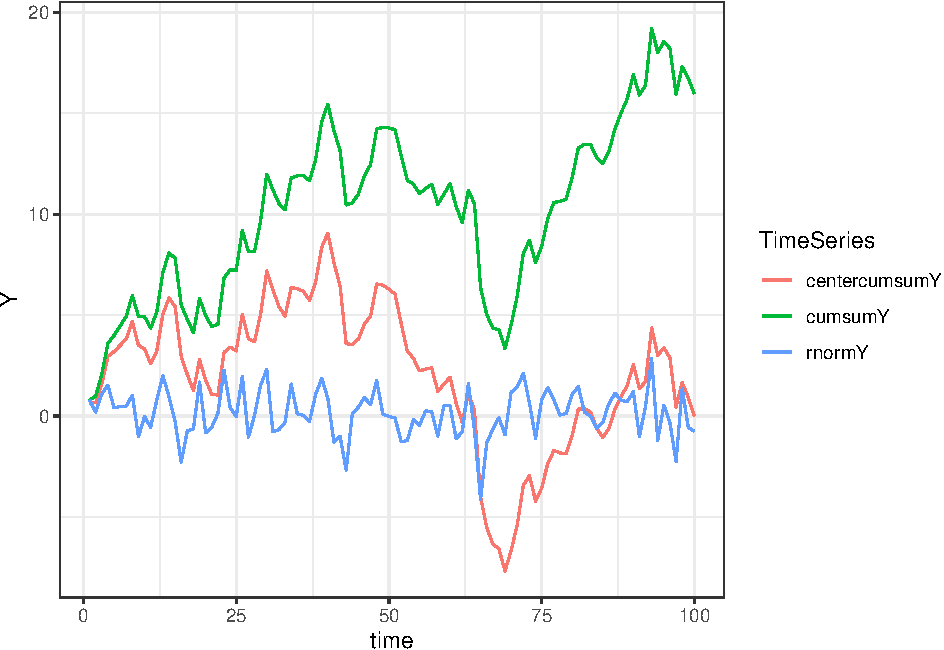
\includegraphics[width=0.99\linewidth]{CSA-Book_files/figure-latex/unnamed-chunk-13-1} \end{center}

\begin{Shaded}
\begin{Highlighting}[]
\CommentTok{# using facets}
\KeywordTok{ggplot}\NormalTok{(df.long, }\KeywordTok{aes}\NormalTok{(}\DataTypeTok{x=}\NormalTok{time,}\DataTypeTok{y=}\NormalTok{Y)) }\OperatorTok{+}
\StringTok{  }\KeywordTok{geom_line}\NormalTok{() }\OperatorTok{+}\StringTok{ }
\StringTok{  }\KeywordTok{facet_wrap}\NormalTok{(}\OperatorTok{~}\NormalTok{TimeSeries) }\OperatorTok{+}
\StringTok{  }\KeywordTok{theme_bw}\NormalTok{()}
\end{Highlighting}
\end{Shaded}

\begin{center}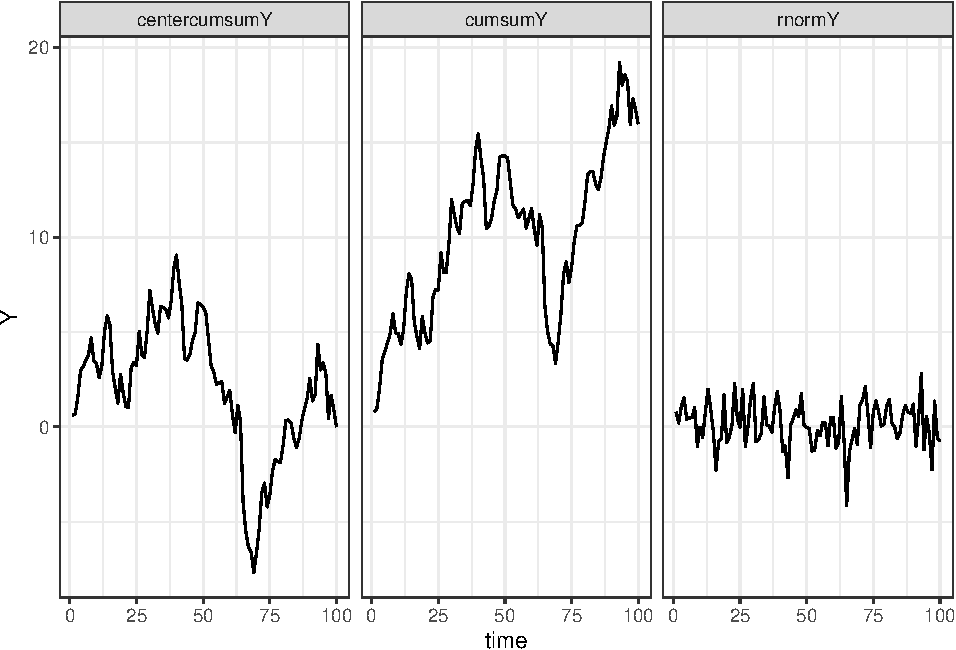
\includegraphics[width=0.99\linewidth]{CSA-Book_files/figure-latex/unnamed-chunk-13-2} \end{center}

\begin{Shaded}
\begin{Highlighting}[]
\CommentTok{# using facets}
\KeywordTok{ggplot}\NormalTok{(df.long, }\KeywordTok{aes}\NormalTok{(}\DataTypeTok{x=}\NormalTok{time,}\DataTypeTok{y=}\NormalTok{Y)) }\OperatorTok{+}
\StringTok{  }\KeywordTok{geom_line}\NormalTok{() }\OperatorTok{+}\StringTok{ }
\StringTok{  }\KeywordTok{facet_grid}\NormalTok{(TimeSeries}\OperatorTok{~}\NormalTok{.) }\OperatorTok{+}
\StringTok{  }\KeywordTok{theme_bw}\NormalTok{()}
\end{Highlighting}
\end{Shaded}

\begin{center}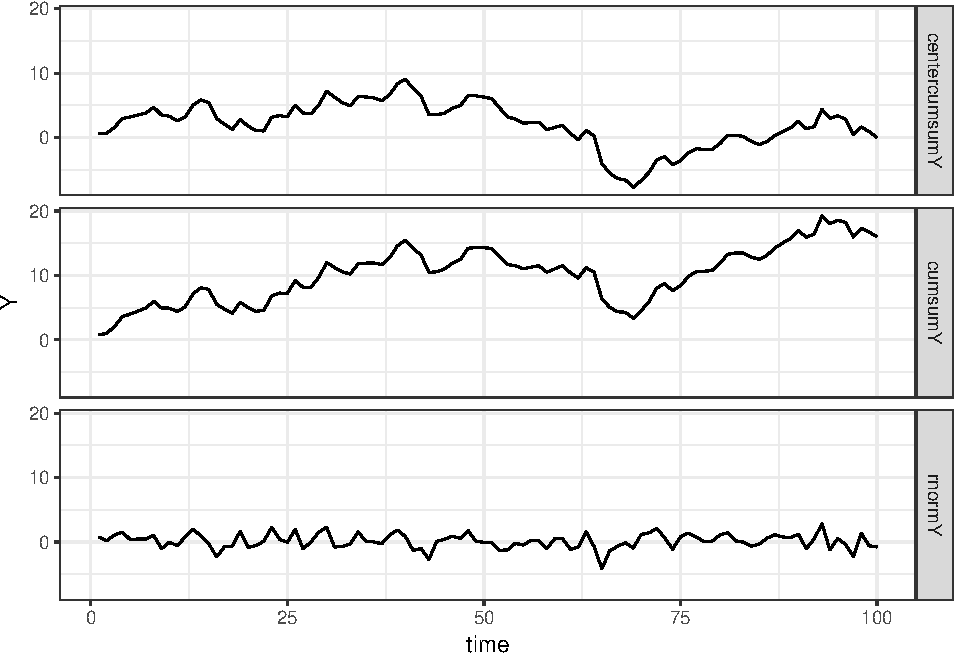
\includegraphics[width=0.99\linewidth]{CSA-Book_files/figure-latex/unnamed-chunk-13-3} \end{center}

To create a return plot you can use \texttt{geom\_path()} instead of \texttt{geom\_line()} and make the area square using \texttt{coord\_equal()}.

\begin{Shaded}
\begin{Highlighting}[]
\CommentTok{# Add a lagged variable}
\NormalTok{df.long <-}\StringTok{ }\NormalTok{df.long }\OperatorTok
\StringTok{  }\KeywordTok{group_by}\NormalTok{(TimeSeries) }\OperatorTok
\StringTok{  }\KeywordTok{mutate}\NormalTok{(}\DataTypeTok{Ylag =}\NormalTok{ dplyr}\OperatorTok{::}\KeywordTok{lag}\NormalTok{(Y))}

\CommentTok{# Use geom-path()}
\KeywordTok{ggplot}\NormalTok{(df.long, }\KeywordTok{aes}\NormalTok{(}\DataTypeTok{x=}\NormalTok{Y,}\DataTypeTok{y=}\NormalTok{Ylag,}\DataTypeTok{group=}\NormalTok{TimeSeries)) }\OperatorTok{+}
\StringTok{  }\KeywordTok{geom_path}\NormalTok{() }\OperatorTok{+}\StringTok{ }
\StringTok{  }\KeywordTok{facet_grid}\NormalTok{(.}\OperatorTok{~}\NormalTok{TimeSeries) }\OperatorTok{+}
\StringTok{  }\KeywordTok{theme_bw}\NormalTok{() }\OperatorTok{+}
\StringTok{  }\KeywordTok{labs}\NormalTok{(}\DataTypeTok{title =} \StringTok{"Equal coordinates"}\NormalTok{, }\DataTypeTok{x=}\StringTok{"Yt"}\NormalTok{,}\DataTypeTok{y=}\StringTok{"Yt+1"}\NormalTok{) }\OperatorTok{+}
\StringTok{  }\KeywordTok{coord_equal}\NormalTok{()}
\end{Highlighting}
\end{Shaded}

\begin{center}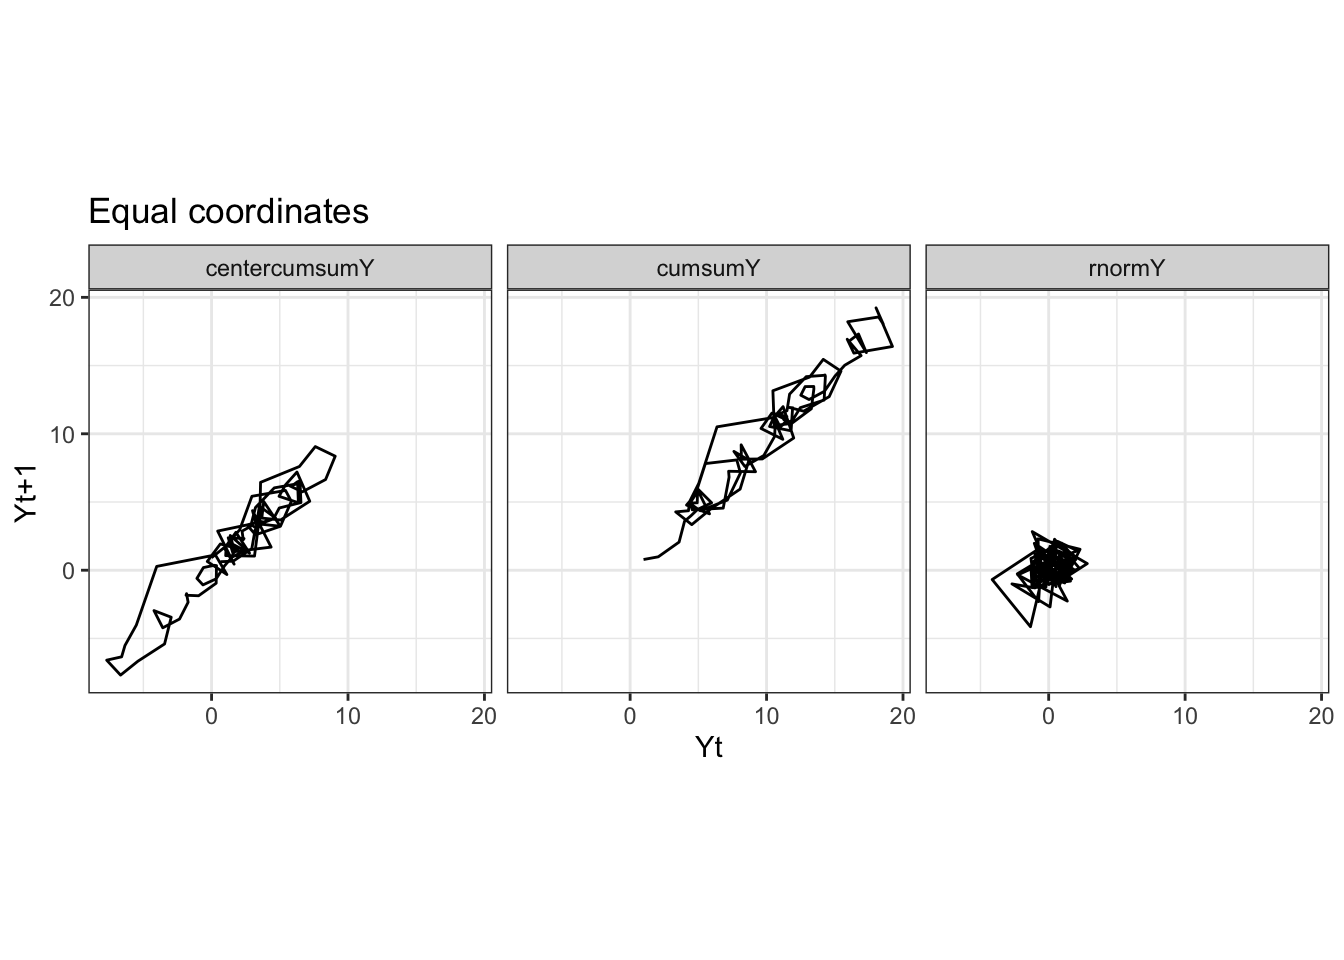
\includegraphics[width=0.99\linewidth]{CSA-Book_files/figure-latex/unnamed-chunk-14-1} \end{center}

\begin{Shaded}
\begin{Highlighting}[]
\CommentTok{# You could also have free axes}
\KeywordTok{ggplot}\NormalTok{(df.long, }\KeywordTok{aes}\NormalTok{(}\DataTypeTok{x=}\NormalTok{Y,}\DataTypeTok{y=}\NormalTok{Ylag,}\DataTypeTok{group=}\NormalTok{TimeSeries)) }\OperatorTok{+}
\StringTok{  }\KeywordTok{geom_path}\NormalTok{() }\OperatorTok{+}\StringTok{ }
\StringTok{  }\KeywordTok{facet_grid}\NormalTok{(.}\OperatorTok{~}\NormalTok{TimeSeries, }\DataTypeTok{scales =} \StringTok{'free'}\NormalTok{) }\OperatorTok{+}
\StringTok{  }\KeywordTok{labs}\NormalTok{(}\DataTypeTok{title=}\StringTok{"Free axes"}\NormalTok{, }\DataTypeTok{x=}\StringTok{"Yt"}\NormalTok{,}\DataTypeTok{y=}\StringTok{"Yt+1"}\NormalTok{) }\OperatorTok{+}
\StringTok{  }\KeywordTok{theme_bw}\NormalTok{() }
\end{Highlighting}
\end{Shaded}

\begin{center}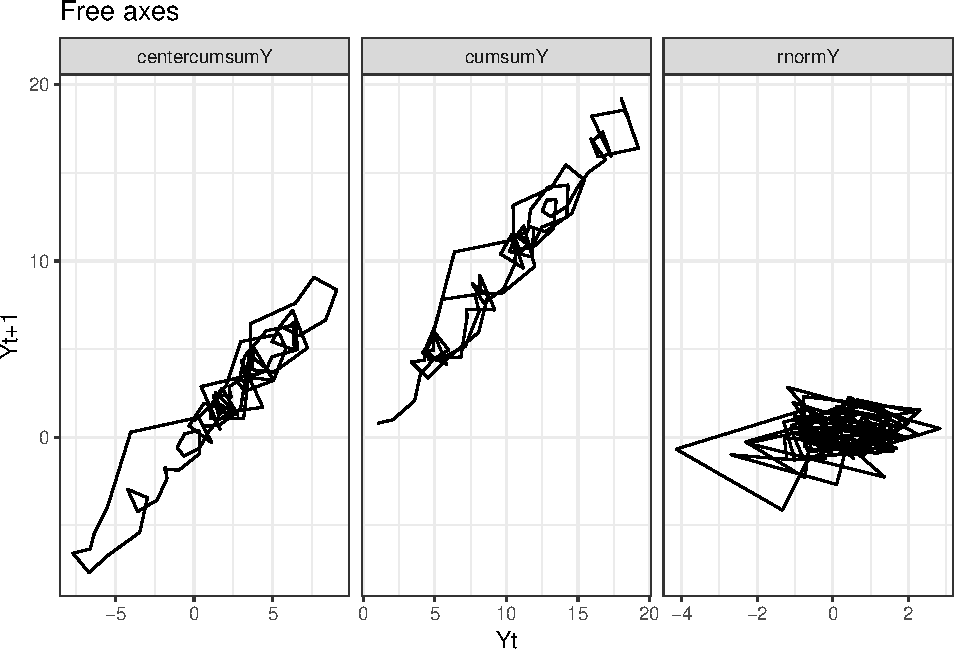
\includegraphics[width=0.99\linewidth]{CSA-Book_files/figure-latex/unnamed-chunk-14-2} \end{center}

\begin{Shaded}
\begin{Highlighting}[]
\CommentTok{# Or free axes and a free space}
\KeywordTok{ggplot}\NormalTok{(df.long, }\KeywordTok{aes}\NormalTok{(}\DataTypeTok{x=}\NormalTok{Y,}\DataTypeTok{y=}\NormalTok{Ylag,}\DataTypeTok{group=}\NormalTok{TimeSeries)) }\OperatorTok{+}
\StringTok{  }\KeywordTok{geom_path}\NormalTok{() }\OperatorTok{+}\StringTok{ }
\StringTok{  }\KeywordTok{facet_grid}\NormalTok{(.}\OperatorTok{~}\NormalTok{TimeSeries, }\DataTypeTok{scales =} \StringTok{'free'}\NormalTok{, }\DataTypeTok{space =} \StringTok{'free'}\NormalTok{) }\OperatorTok{+}
\StringTok{  }\KeywordTok{labs}\NormalTok{(}\DataTypeTok{title=}\StringTok{"Free axes and free space"}\NormalTok{, }\DataTypeTok{x=}\StringTok{"Yt"}\NormalTok{,}\DataTypeTok{y=}\StringTok{"Yt+1"}\NormalTok{) }\OperatorTok{+}
\StringTok{  }\KeywordTok{theme_bw}\NormalTok{() }
\end{Highlighting}
\end{Shaded}

\begin{center}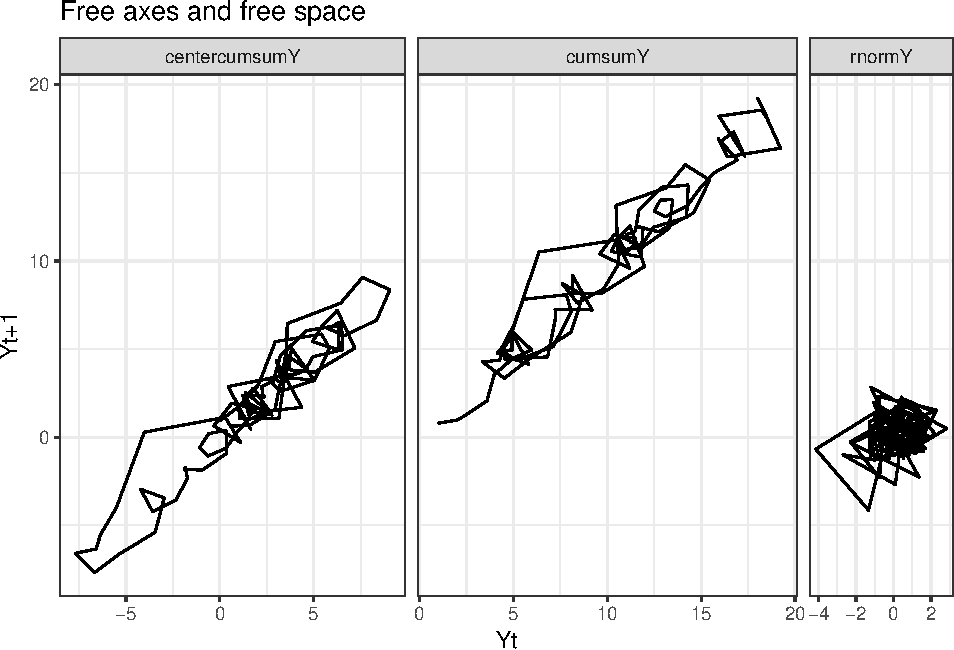
\includegraphics[width=0.99\linewidth]{CSA-Book_files/figure-latex/unnamed-chunk-14-3} \end{center}

\hypertarget{implementing-iterative-functions}{%
\section{\texorpdfstring{\textbf{Implementing iterative functions}}{Implementing iterative functions}}\label{implementing-iterative-functions}}

Coding change processes (difference equations) in \texttt{Matlab} and \texttt{R} is always easier than using a spreadsheet. One obvious way to do it is to use a counter variable representing the iterations of time in a \texttt{for\ ...\ next} loop (see \protect\hyperlink{tutorials}{tutorials}). The iterations should run over a vector (which is the same concept as a row or a column in a spreadsheet: An indexed array of numbers or characters). The first entry should be the starting value, so the vector index \(1\) represents \(Y_0\).

The loop can be implemented a number of ways, for example as a function which can be called from a script or the command or console window. In \texttt{R} working with \textbf{functions} is easy, and very much recommended (see \protect\hyperlink{tutorials}{tutorials}), because it will speed up calculations considerably, and it will reduce the amount of code you need to write. You need to gain some experience with coding in \texttt{R} before you'll get it right. In order to get it lean and clean (and possibly even mean as well) you'll need a lot of experience with coding in \texttt{R},therefore, we will (eventually) provide you the functions you'll need to complete the assignments in the \textbf{Answers} section of the assignments. If you get stuck, look at the answers. If you need to do something that reminds you of an assignment, figure out how to modify the answers to suit your specific needs.

We'll use the linear map \(Y_{i+1} = r*Y_i\) as an example and show three different ways to implement iterative processes:

\begin{enumerate}
\def\labelenumi{\arabic{enumi}.}
\tightlist
\item
  The \texttt{for...} loop
\item
  The \texttt{-ply} family of functions
\item
  User defined \texttt{function()} with arguments
\end{enumerate}

\begin{Shaded}
\begin{Highlighting}[]
\CommentTok{# for loop}
\NormalTok{N  <-}\StringTok{ }\DecValTok{100}
\NormalTok{r  <-}\StringTok{ }\FloatTok{-.9}
\NormalTok{Y0 <-}\StringTok{ }\FloatTok{0.01}
\NormalTok{Y  <-}\StringTok{ }\KeywordTok{c}\NormalTok{(Y0,}\KeywordTok{rep}\NormalTok{(}\OtherTok{NA}\NormalTok{,N}\DecValTok{-1}\NormalTok{))}

\ControlFlowTok{for}\NormalTok{(i }\ControlFlowTok{in} \DecValTok{1}\OperatorTok{:}\NormalTok{(N}\DecValTok{-1}\NormalTok{))\{}
\NormalTok{  Y[i}\OperatorTok{+}\DecValTok{1}\NormalTok{] <-}\StringTok{ }\NormalTok{r}\OperatorTok{*}\NormalTok{Y[i]}
\NormalTok{\}}
\KeywordTok{plot}\NormalTok{(Y,}\DataTypeTok{type =} \StringTok{"l"}\NormalTok{)}
\end{Highlighting}
\end{Shaded}

\begin{center}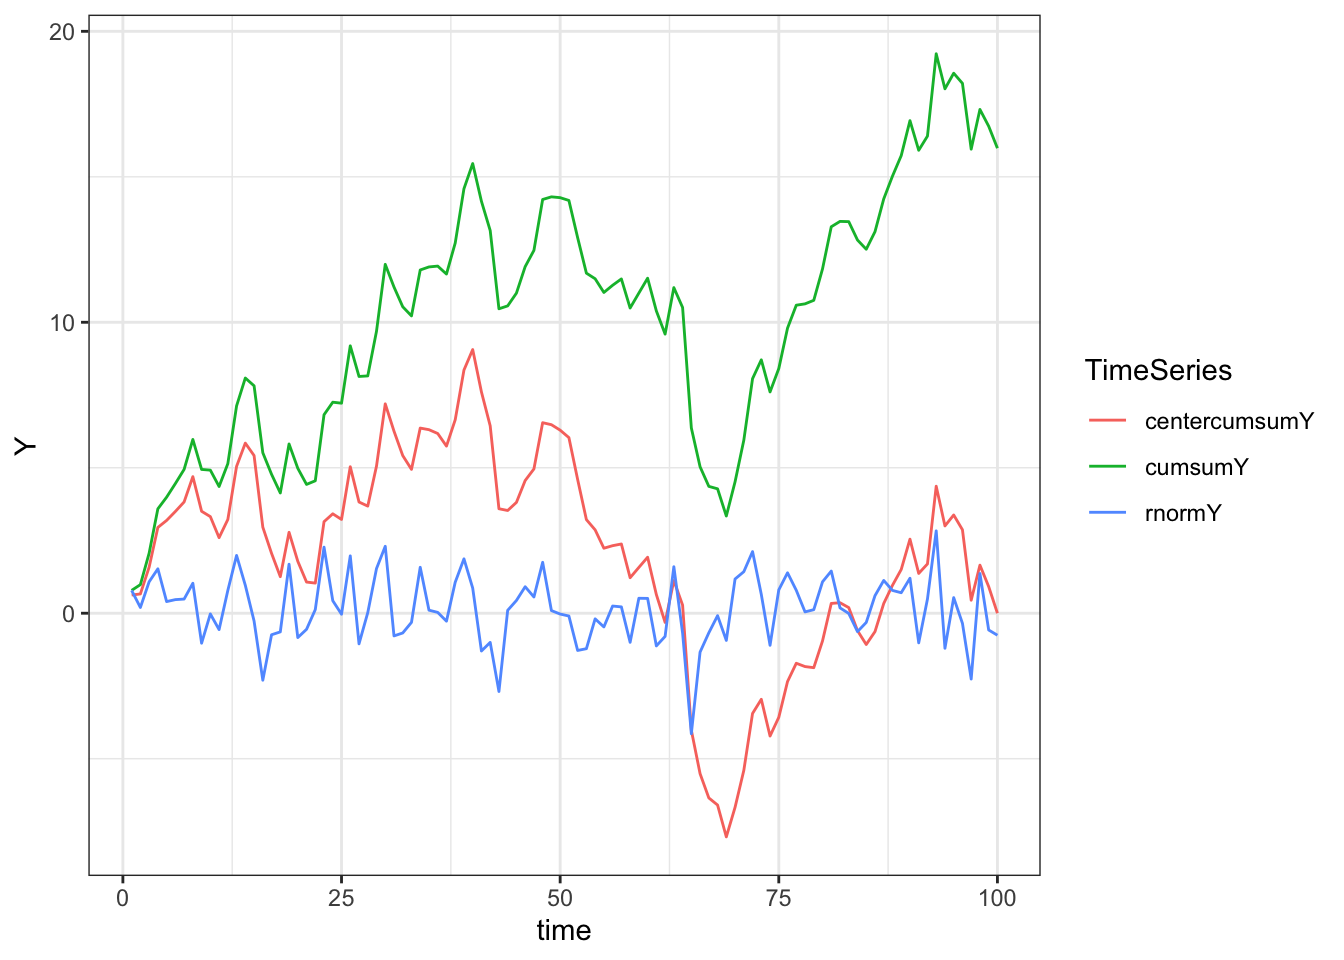
\includegraphics[width=0.99\linewidth]{CSA-Book_files/figure-latex/unnamed-chunk-15-1} \end{center}

\begin{Shaded}
\begin{Highlighting}[]
\CommentTok{# -ply family: sapply}
\NormalTok{Yout <-}\StringTok{ }\KeywordTok{sapply}\NormalTok{(}\KeywordTok{seq_along}\NormalTok{(Y),}\ControlFlowTok{function}\NormalTok{(t) r}\OperatorTok{*}\NormalTok{Y[t])}
\KeywordTok{plot}\NormalTok{(Yout,}\DataTypeTok{type =} \StringTok{"l"}\NormalTok{)}
\end{Highlighting}
\end{Shaded}

\begin{center}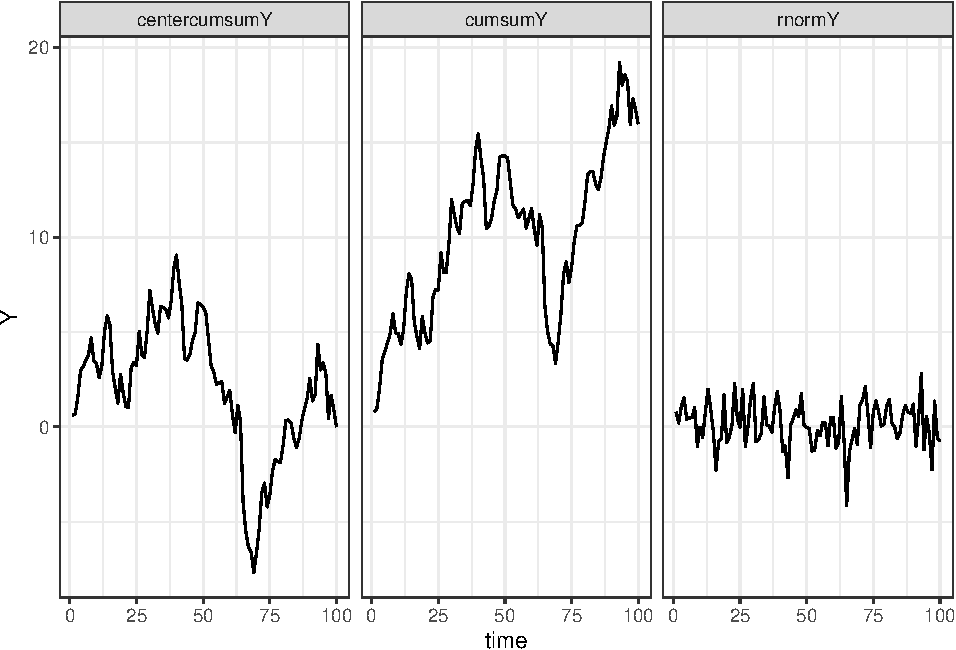
\includegraphics[width=0.99\linewidth]{CSA-Book_files/figure-latex/unnamed-chunk-15-2} \end{center}

\begin{Shaded}
\begin{Highlighting}[]
\CommentTok{# function with for loop}
\NormalTok{linmap1 <-}\StringTok{ }\ControlFlowTok{function}\NormalTok{(Y0,r,N)\{}
\NormalTok{  Y  <-}\StringTok{ }\KeywordTok{c}\NormalTok{(Y0,}\KeywordTok{rep}\NormalTok{(}\OtherTok{NA}\NormalTok{,N}\DecValTok{-1}\NormalTok{))}
  \ControlFlowTok{for}\NormalTok{(i }\ControlFlowTok{in} \DecValTok{1}\OperatorTok{:}\NormalTok{(N}\DecValTok{-1}\NormalTok{))\{}
\NormalTok{    Y[i}\OperatorTok{+}\DecValTok{1}\NormalTok{] <-}\StringTok{ }\NormalTok{r}\OperatorTok{*}\NormalTok{Y[i]}
\NormalTok{  \}}
  \KeywordTok{return}\NormalTok{(Y)}
\NormalTok{\}}
\KeywordTok{plot}\NormalTok{(}\KeywordTok{linmap1}\NormalTok{(Y0,r,N),}\DataTypeTok{type =} \StringTok{"l"}\NormalTok{)}
\end{Highlighting}
\end{Shaded}

\begin{center}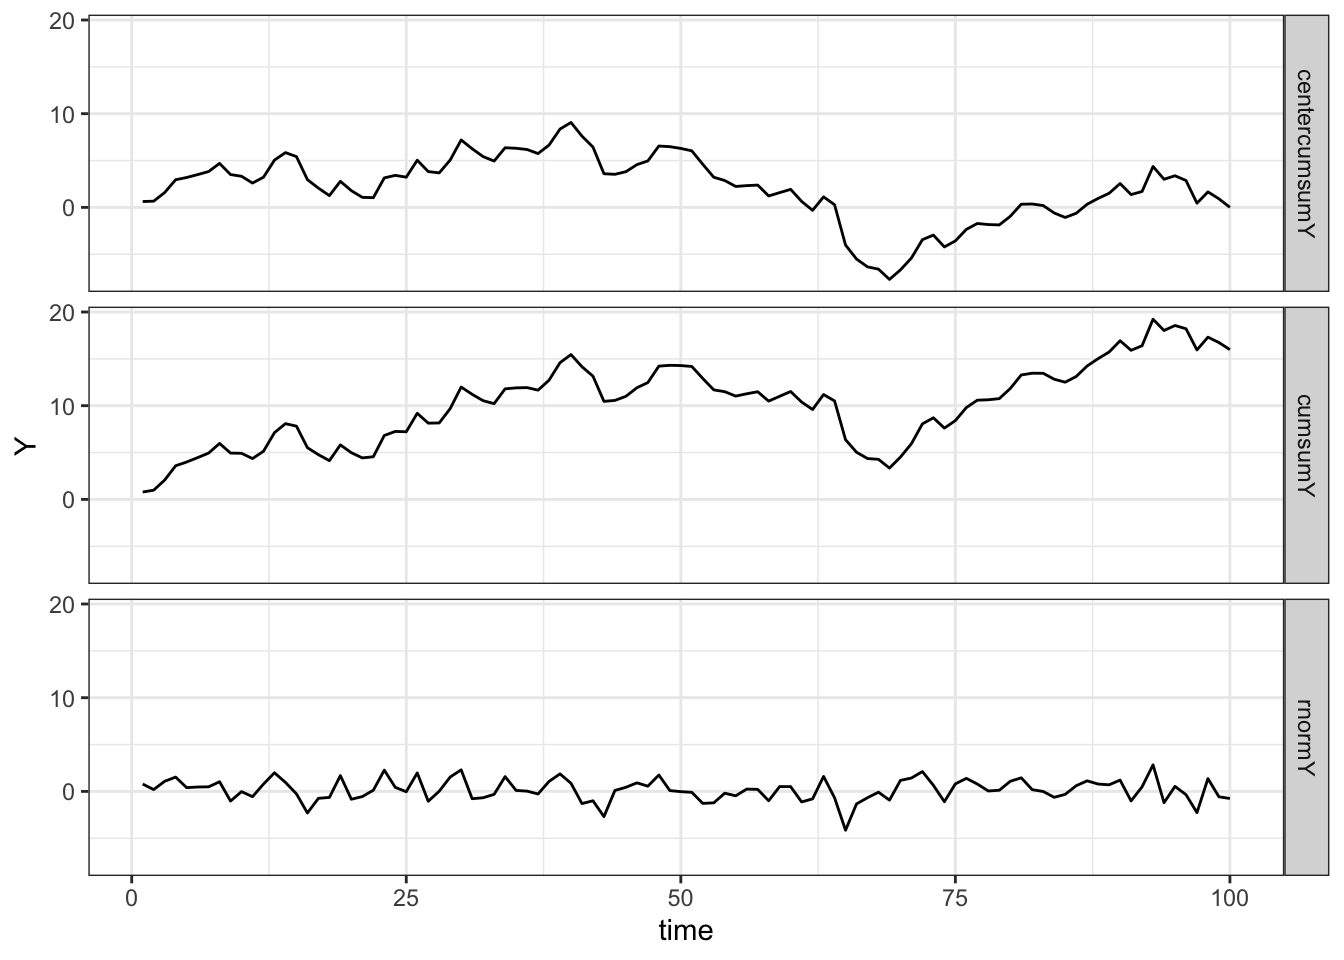
\includegraphics[width=0.99\linewidth]{CSA-Book_files/figure-latex/unnamed-chunk-15-3} \end{center}

\hypertarget{numerical-integration-to-simulate-continuous-time}{%
\section{\texorpdfstring{\textbf{Numerical integration to simulate continuous time}}{Numerical integration to simulate continuous time}}\label{numerical-integration-to-simulate-continuous-time}}

In order to `solve' a differential equation for continuous time using a method of numerical integration, one could code it like in the spreadsheet assignment below. For \texttt{R} and \texttt{Matlab} there are so-called \emph{solvers} available, functions that will do the integration for you. For \texttt{R} look at the \href{http://desolve.r-forge.r-project.org}{Examples in package \texttt{deSolve}}.

\hypertarget{eulers-method-and-more}{%
\subsection*{Euler's method and more\ldots{}}\label{eulers-method-and-more}}
\addcontentsline{toc}{subsection}{Euler's method and more\ldots{}}

The result of applying a method of numerical integration is called a \textbf{numerical solution} of the differential equation. The \textbf{analytical solution} is the equation which will give you a value of \(Y\) for any point in time, given an initial value \(Y_0\). Systems which have an analytical solution can be used to test the accuracy of \textbf{numerical solutions}.

\hypertarget{analytical-solution}{%
\subsection*{Analytical solution}\label{analytical-solution}}
\addcontentsline{toc}{subsection}{Analytical solution}

Remember that the analytical solution for the logistic equation is:

\[
Y(t)  =  \frac{K * Y_0}{Y_0 + \left(K - Y_0 \right) * e^{-r*t} }
\]
This can be `simplified' to

\[
Y(t)  =  \frac{K}{1 + \left(\frac{K}{Y_0-1} \right) * e^{-r*t} }
\]

If we want to know the growth level \(Y_t\) at \(t=10\), with \(Y_0=.0001\), \(r=1.1\) and \(K=4\), we can just \texttt{fill\ it\ in}:

\begin{Shaded}
\begin{Highlighting}[]
\CommentTok{# Define a function for the solution}
\NormalTok{logSol <-}\StringTok{ }\ControlFlowTok{function}\NormalTok{(Y0, r, K, t)\{K}\OperatorTok{/}\NormalTok{(}\DecValTok{1}\OperatorTok{+}\NormalTok{(K}\OperatorTok{/}\NormalTok{Y0}\DecValTok{-1}\NormalTok{)}\OperatorTok{*}\KeywordTok{exp}\NormalTok{(}\OperatorTok{-}\NormalTok{r}\OperatorTok{*}\NormalTok{t))\}}

\CommentTok{# Call the function}
\KeywordTok{logSol}\NormalTok{(}\DataTypeTok{Y0=}\NormalTok{.}\DecValTok{0001}\NormalTok{, }\DataTypeTok{r=}\FloatTok{1.1}\NormalTok{, }\DataTypeTok{K=}\DecValTok{4}\NormalTok{, }\DataTypeTok{t=}\DecValTok{10}\NormalTok{)}
\end{Highlighting}
\end{Shaded}

\begin{verbatim}
## [1] 2.398008
\end{verbatim}

We can pass a vector of time points to create the exact solution, the same we would get if we were to iterate the differential/difference equation.

\begin{Shaded}
\begin{Highlighting}[]
\CommentTok{# Plot from t=1 to t=100}
\KeywordTok{plot}\NormalTok{(}\KeywordTok{logSol}\NormalTok{(}\DataTypeTok{Y0=}\NormalTok{.}\DecValTok{0001}\NormalTok{, }\DataTypeTok{r=}\FloatTok{1.1}\NormalTok{, }\DataTypeTok{K=}\DecValTok{4}\NormalTok{, }\DataTypeTok{t=}\KeywordTok{seq}\NormalTok{(}\DecValTok{1}\NormalTok{,}\DecValTok{20}\NormalTok{)), }\DataTypeTok{type =} \StringTok{"b"}\NormalTok{, }
     \DataTypeTok{ylab =} \KeywordTok{expression}\NormalTok{(Y[t]), }\DataTypeTok{xlab =} \StringTok{"t"}\NormalTok{)}
\CommentTok{# Plot t=10 in red}
\KeywordTok{points}\NormalTok{(}\DecValTok{10}\NormalTok{,}\KeywordTok{logSol}\NormalTok{(}\DataTypeTok{Y0=}\NormalTok{.}\DecValTok{0001}\NormalTok{, }\DataTypeTok{r=}\FloatTok{1.1}\NormalTok{, }\DataTypeTok{K=}\DecValTok{4}\NormalTok{, }\DataTypeTok{t=}\DecValTok{10}\NormalTok{), }\DataTypeTok{col=}\StringTok{"red"}\NormalTok{, }\DataTypeTok{pch=}\DecValTok{16}\NormalTok{)}
\end{Highlighting}
\end{Shaded}

\begin{center}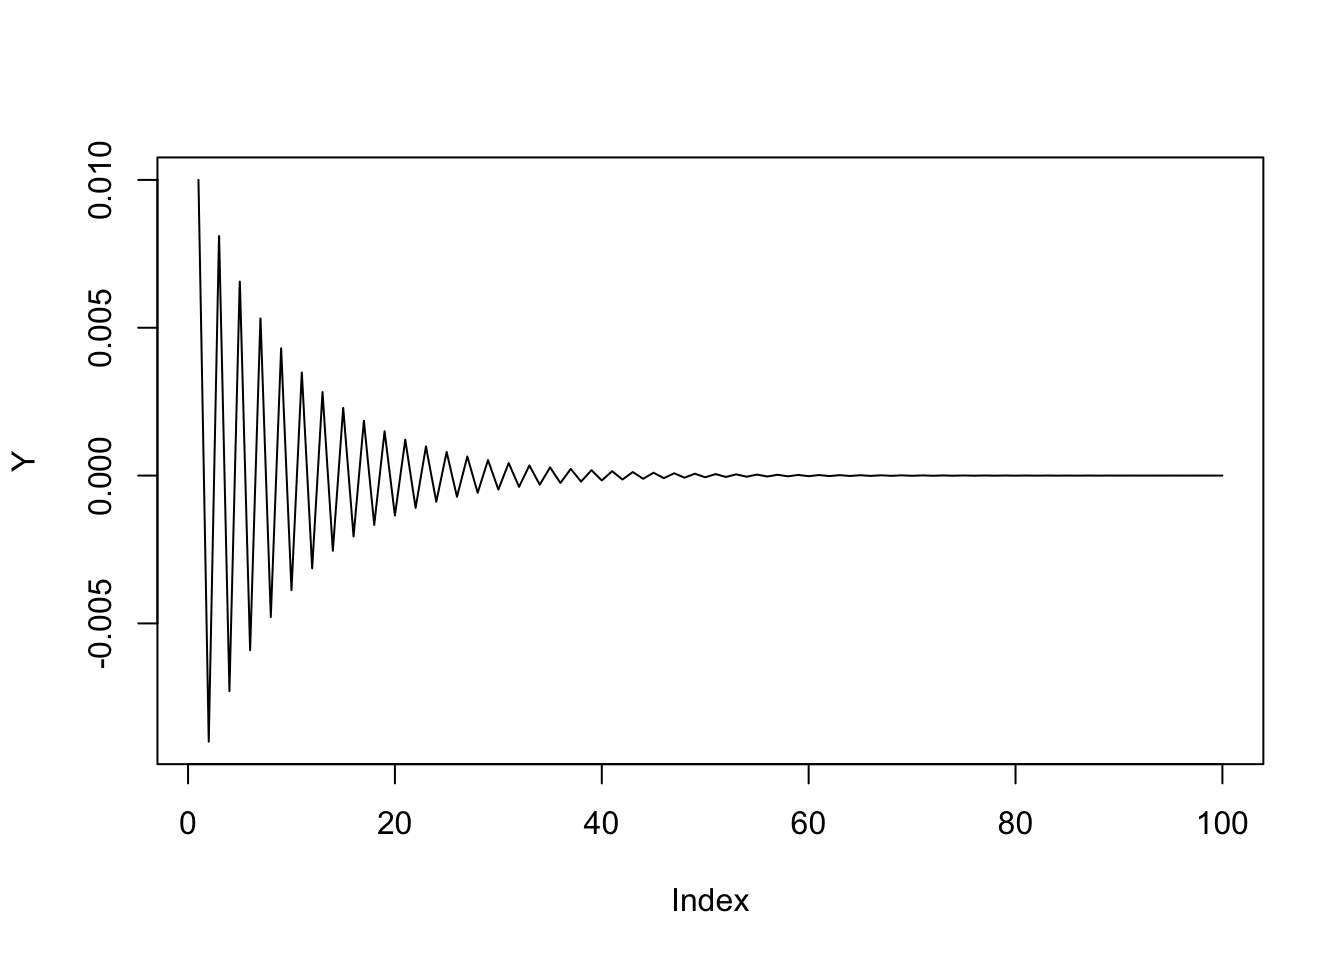
\includegraphics[width=0.99\linewidth]{CSA-Book_files/figure-latex/unnamed-chunk-17-1} \end{center}

\hypertarget{numerical-solution-discrete}{%
\subsection*{Numerical solution (discrete)}\label{numerical-solution-discrete}}
\addcontentsline{toc}{subsection}{Numerical solution (discrete)}

If we would iterate the differential equation \ldots{}

\[
\frac{dY}{dt} = Y_t * (1 + r - r * \frac{Y_t}{K})
\]

\ldots{} as if it were a difference equation, we are \emph{not} simulating continuous time, but a discrete time version of the model:

\[
Y_{i+1} = Y_i * (1 + r - r * \frac{Y_i}{K})
\]

\begin{Shaded}
\begin{Highlighting}[]
\NormalTok{logIter <-}\StringTok{  }\ControlFlowTok{function}\NormalTok{(Y0,r,K,t)\{}
\NormalTok{  N <-}\StringTok{ }\KeywordTok{length}\NormalTok{(t)}
\NormalTok{  Y <-}\StringTok{ }\KeywordTok{as.numeric}\NormalTok{(}\KeywordTok{c}\NormalTok{(Y0, }\KeywordTok{rep}\NormalTok{(}\OtherTok{NA}\NormalTok{,N}\DecValTok{-2}\NormalTok{)))}
  \KeywordTok{sapply}\NormalTok{(}\KeywordTok{seq_along}\NormalTok{(Y), }\ControlFlowTok{function}\NormalTok{(t)\{ Y[[t}\OperatorTok{+}\DecValTok{1}\NormalTok{]] <<-}\StringTok{ }\NormalTok{Y[t] }\OperatorTok{*}\StringTok{ }\NormalTok{(}\DecValTok{1} \OperatorTok{+}\StringTok{ }\NormalTok{r }\OperatorTok{-}\StringTok{ }\NormalTok{r }\OperatorTok{*}\StringTok{ }\NormalTok{Y[t] }\OperatorTok{/}\StringTok{ }\NormalTok{K)\})}
\NormalTok{  \}}

\CommentTok{# Plot from t=1 to t=100}
\KeywordTok{plot}\NormalTok{(}\KeywordTok{logIter}\NormalTok{(}\DataTypeTok{Y0=}\NormalTok{.}\DecValTok{0001}\NormalTok{, }\DataTypeTok{r=}\FloatTok{1.1}\NormalTok{, }\DataTypeTok{K=}\DecValTok{4}\NormalTok{, }\DataTypeTok{t=}\KeywordTok{seq}\NormalTok{(}\DecValTok{1}\NormalTok{,}\DecValTok{20}\NormalTok{)), }\DataTypeTok{type =} \StringTok{"b"}\NormalTok{, }
     \DataTypeTok{ylab =} \KeywordTok{expression}\NormalTok{(Y[t]), }\DataTypeTok{xlab =} \StringTok{"t"}\NormalTok{)}
\CommentTok{# Plot t=10 in red}
\KeywordTok{points}\NormalTok{(}\DecValTok{10}\NormalTok{,}\KeywordTok{logSol}\NormalTok{(}\DataTypeTok{Y0=}\NormalTok{.}\DecValTok{0001}\NormalTok{, }\DataTypeTok{r=}\FloatTok{1.1}\NormalTok{, }\DataTypeTok{K=}\DecValTok{4}\NormalTok{, }\DataTypeTok{t=}\DecValTok{10}\NormalTok{), }\DataTypeTok{col=}\StringTok{"red"}\NormalTok{, }\DataTypeTok{pch=}\DecValTok{16}\NormalTok{)}
\end{Highlighting}
\end{Shaded}

\begin{center}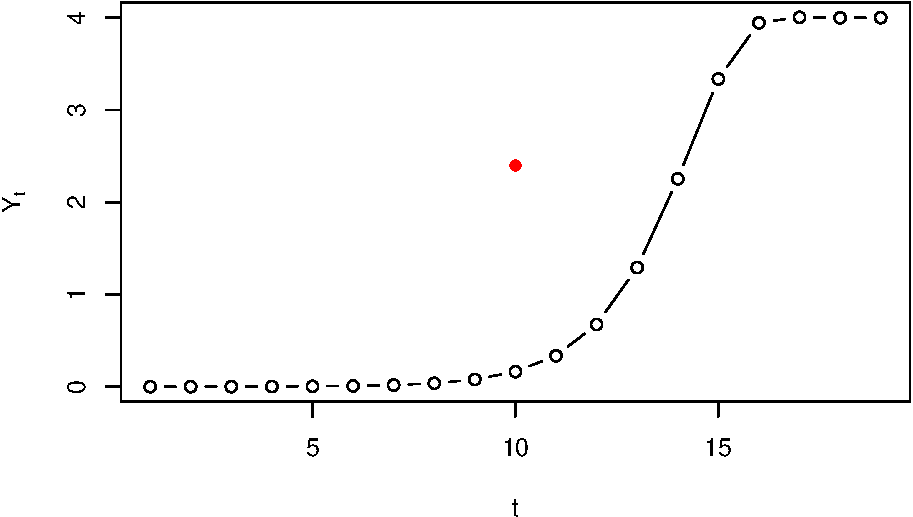
\includegraphics[width=0.99\linewidth]{CSA-Book_files/figure-latex/unnamed-chunk-18-1} \end{center}

\hypertarget{euler-vs.runge-kutta}{%
\subsection{Euler vs.~Runge-Kutta}\label{euler-vs.runge-kutta}}

The method developped by Runge and Kutta takes a harmonic mean over a number of points, R-K4 takes 4 points, R-K6 takes 6, \href{https://en.wikipedia.org/wiki/Runge–Kutta_methods}{but there are many more variants}.

Here's an exampkle with \textbf{Predator-Prey dynamics} comparing Euler's method to R-K4.

\begin{Shaded}
\begin{Highlighting}[]
\KeywordTok{library}\NormalTok{(plyr)}
\KeywordTok{library}\NormalTok{(tidyverse)}
\KeywordTok{library}\NormalTok{(lattice)}

\CommentTok{# Lotka-Volterra Euler}
\NormalTok{lvEuler <-}\StringTok{ }\ControlFlowTok{function}\NormalTok{(R0,F0,N,a,b,c,d,h)\{}

  \CommentTok{# Init vector}
\NormalTok{  Ra <-}\StringTok{ }\KeywordTok{as.numeric}\NormalTok{(}\KeywordTok{c}\NormalTok{(R0, }\KeywordTok{rep}\NormalTok{(}\OtherTok{NA}\NormalTok{,N}\DecValTok{-1}\NormalTok{)))}
\NormalTok{  Fx <-}\StringTok{ }\KeywordTok{as.numeric}\NormalTok{(}\KeywordTok{c}\NormalTok{(F0, }\KeywordTok{rep}\NormalTok{(}\OtherTok{NA}\NormalTok{,N}\DecValTok{-1}\NormalTok{)))}

  \ControlFlowTok{for}\NormalTok{(t }\ControlFlowTok{in} \DecValTok{1}\OperatorTok{:}\NormalTok{N)\{}
  \CommentTok{# Euler numerical solution of the predator-prey model}
\NormalTok{  Ra[t}\OperatorTok{+}\DecValTok{1}\NormalTok{] <-}\StringTok{ }\NormalTok{Ra[t] }\OperatorTok{+}\StringTok{ }\NormalTok{(a }\OperatorTok{-}\StringTok{ }\NormalTok{b }\OperatorTok{*}\StringTok{ }\NormalTok{Fx[t]) }\OperatorTok{*}\StringTok{ }\NormalTok{Ra[t] }\OperatorTok{*}\StringTok{ }\NormalTok{h}
\NormalTok{  Fx[t}\OperatorTok{+}\DecValTok{1}\NormalTok{] <-}\StringTok{ }\NormalTok{Fx[t] }\OperatorTok{+}\StringTok{ }\NormalTok{(c }\OperatorTok{*}\StringTok{ }\NormalTok{Ra[t] }\OperatorTok{-}\StringTok{ }\NormalTok{d) }\OperatorTok{*}\StringTok{ }\NormalTok{Fx[t] }\OperatorTok{*}\StringTok{ }\NormalTok{h}
\NormalTok{  \}}
  
  \KeywordTok{return}\NormalTok{(}\KeywordTok{data.frame}\NormalTok{(}\DataTypeTok{time=}\DecValTok{1}\OperatorTok{:}\KeywordTok{NROW}\NormalTok{(Ra),}\DataTypeTok{Ra=}\NormalTok{Ra,}\DataTypeTok{Fx=}\NormalTok{Fx,}\DataTypeTok{method=}\StringTok{"Euler"}\NormalTok{))}
\NormalTok{\}}

\CommentTok{# Lotka-Volterra Runge Kutta 4}
\NormalTok{lvRK4 <-}\StringTok{ }\ControlFlowTok{function}\NormalTok{(R0,F0,N,a,b,c,d,h)\{}

  \CommentTok{# Init vector}
\NormalTok{  Ra <-}\StringTok{ }\KeywordTok{as.numeric}\NormalTok{(}\KeywordTok{c}\NormalTok{(R0, }\KeywordTok{rep}\NormalTok{(}\OtherTok{NA}\NormalTok{,N}\DecValTok{-1}\NormalTok{)))}
\NormalTok{  Fx <-}\StringTok{ }\KeywordTok{as.numeric}\NormalTok{(}\KeywordTok{c}\NormalTok{(F0, }\KeywordTok{rep}\NormalTok{(}\OtherTok{NA}\NormalTok{,N}\DecValTok{-1}\NormalTok{)))}

  \ControlFlowTok{for}\NormalTok{(t }\ControlFlowTok{in} \DecValTok{1}\OperatorTok{:}\NormalTok{N)\{}
  \CommentTok{# RK4 numerical solution of the predator-prey model}
\NormalTok{  k1_R=(a }\OperatorTok{-}\StringTok{ }\NormalTok{b }\OperatorTok{*}\StringTok{ }\NormalTok{Fx[t]) }\OperatorTok{*}\StringTok{ }\NormalTok{Ra[t]}
\NormalTok{  k1_F=(c }\OperatorTok{*}\StringTok{ }\NormalTok{Ra[t] }\OperatorTok{-}\StringTok{ }\NormalTok{d) }\OperatorTok{*}\StringTok{ }\NormalTok{Fx[t]}

\NormalTok{  k2_R=(a }\OperatorTok{-}\StringTok{ }\NormalTok{b }\OperatorTok{*}\StringTok{ }\NormalTok{(Fx[t]}\OperatorTok{+}\NormalTok{h}\OperatorTok{*}\NormalTok{k1_F}\OperatorTok{/}\DecValTok{2}\NormalTok{)) }\OperatorTok{*}\StringTok{ }\NormalTok{(Ra[t]}\OperatorTok{+}\NormalTok{h}\OperatorTok{*}\NormalTok{k1_R}\OperatorTok{/}\DecValTok{2}\NormalTok{)}
\NormalTok{  k2_F=(c }\OperatorTok{*}\StringTok{ }\NormalTok{(Ra[t]}\OperatorTok{+}\NormalTok{h}\OperatorTok{*}\NormalTok{k1_R}\OperatorTok{/}\DecValTok{2}\NormalTok{) }\OperatorTok{-}\StringTok{ }\NormalTok{d) }\OperatorTok{*}\StringTok{ }\NormalTok{(Fx[t]}\OperatorTok{+}\NormalTok{h}\OperatorTok{*}\NormalTok{k1_F}\OperatorTok{/}\DecValTok{2}\NormalTok{)}

\NormalTok{  k3_R=(a }\OperatorTok{-}\StringTok{ }\NormalTok{b }\OperatorTok{*}\StringTok{ }\NormalTok{(Fx[t]}\OperatorTok{+}\NormalTok{h}\OperatorTok{*}\NormalTok{k2_F}\OperatorTok{/}\DecValTok{2}\NormalTok{)) }\OperatorTok{*}\StringTok{ }\NormalTok{(Ra[t]}\OperatorTok{+}\NormalTok{h}\OperatorTok{*}\NormalTok{k2_R}\OperatorTok{/}\DecValTok{2}\NormalTok{)}
\NormalTok{  k3_F=(c }\OperatorTok{*}\StringTok{ }\NormalTok{(Ra[t]}\OperatorTok{+}\NormalTok{h}\OperatorTok{*}\NormalTok{k2_R}\OperatorTok{/}\DecValTok{2}\NormalTok{) }\OperatorTok{-}\StringTok{ }\NormalTok{d) }\OperatorTok{*}\StringTok{ }\NormalTok{(Fx[t]}\OperatorTok{+}\NormalTok{h}\OperatorTok{*}\NormalTok{k2_F}\OperatorTok{/}\DecValTok{2}\NormalTok{)}

\NormalTok{  k4_R=(a }\OperatorTok{-}\StringTok{ }\NormalTok{b }\OperatorTok{*}\StringTok{ }\NormalTok{(Fx[t]}\OperatorTok{+}\NormalTok{h}\OperatorTok{*}\NormalTok{k3_F)) }\OperatorTok{*}\StringTok{ }\NormalTok{(Ra[t]}\OperatorTok{+}\NormalTok{h}\OperatorTok{*}\NormalTok{k3_R)}
\NormalTok{  k4_F=(c }\OperatorTok{*}\StringTok{ }\NormalTok{(Ra[t]}\OperatorTok{+}\NormalTok{h}\OperatorTok{*}\NormalTok{k3_R) }\OperatorTok{-}\StringTok{ }\NormalTok{d) }\OperatorTok{*}\StringTok{ }\NormalTok{(Fx[t]}\OperatorTok{+}\NormalTok{h}\OperatorTok{*}\NormalTok{k3_F)}

  \CommentTok{# Iterative process}
\NormalTok{  Ra[t}\OperatorTok{+}\DecValTok{1}\NormalTok{] <-}\StringTok{ }\NormalTok{Ra[t] }\OperatorTok{+}\StringTok{ }\NormalTok{(}\DecValTok{1}\OperatorTok{/}\DecValTok{6}\NormalTok{)}\OperatorTok{*}\NormalTok{h}\OperatorTok{*}\NormalTok{(k1_R}\OperatorTok{+}\DecValTok{2}\OperatorTok{*}\NormalTok{k2_R}\OperatorTok{+}\DecValTok{2}\OperatorTok{*}\NormalTok{k3_R}\OperatorTok{+}\NormalTok{k4_R)}
\NormalTok{  Fx[t}\OperatorTok{+}\DecValTok{1}\NormalTok{] <-}\StringTok{ }\NormalTok{Fx[t] }\OperatorTok{+}\StringTok{ }\NormalTok{(}\DecValTok{1}\OperatorTok{/}\DecValTok{6}\NormalTok{)}\OperatorTok{*}\NormalTok{h}\OperatorTok{*}\NormalTok{(k1_F}\OperatorTok{+}\DecValTok{2}\OperatorTok{*}\NormalTok{k2_F}\OperatorTok{+}\DecValTok{2}\OperatorTok{*}\NormalTok{k3_F}\OperatorTok{+}\NormalTok{k4_F)}
\NormalTok{  \}}
  
  \KeywordTok{return}\NormalTok{(}\KeywordTok{data.frame}\NormalTok{(}\DataTypeTok{time=}\DecValTok{1}\OperatorTok{:}\KeywordTok{NROW}\NormalTok{(Ra),}\DataTypeTok{Ra=}\NormalTok{Ra,}\DataTypeTok{Fx=}\NormalTok{Fx,}\DataTypeTok{method=}\StringTok{"RK4"}\NormalTok{))}
\NormalTok{\}}
\end{Highlighting}
\end{Shaded}

Now that we have the fuctions, we'll plot the numerical solutions for the same set of parameters. The continuous mathematics (= if you do some calculations to find the fixed points of the system) ensure us that the system should be in an equilibrium state in which the populations keep going around in the same cycle of growth and collapse. Let's see what happens\ldots{}

\begin{Shaded}
\begin{Highlighting}[]
\CommentTok{# Parameters}
\NormalTok{N  <-}\StringTok{ }\DecValTok{2000}

\CommentTok{# Equilibrium}
\NormalTok{a  <-}\StringTok{ }\DecValTok{1}\OperatorTok{/}\DecValTok{6}
\NormalTok{b  <-}\StringTok{ }\DecValTok{4}\OperatorTok{/}\DecValTok{3}
\NormalTok{c  <-}\StringTok{ }\NormalTok{d  <-}\StringTok{ }\DecValTok{1}
\NormalTok{R0 <-}\StringTok{ }\NormalTok{F0 <-}\StringTok{ }\FloatTok{0.1}

\CommentTok{# Time constant}
\NormalTok{h <-}\StringTok{ }\FloatTok{0.1}

\CommentTok{# Get the results}
\NormalTok{pp1 <-}\StringTok{ }\KeywordTok{lvEuler}\NormalTok{(R0,F0,N,a,b,c,d,h)}
\NormalTok{pp2 <-}\StringTok{ }\KeywordTok{lvRK4}\NormalTok{(R0,F0,N,a,b,c,d,h)}

\CommentTok{# Make a long dataframe}
\NormalTok{pp <-}\StringTok{ }\KeywordTok{rbind}\NormalTok{(pp1,pp2)}

\NormalTok{pp.long <-}\StringTok{ }\NormalTok{pp }\OperatorTok
\StringTok{  }\KeywordTok{gather}\NormalTok{(}\DataTypeTok{key =}\NormalTok{ TimeSeries, }\DataTypeTok{value =}\NormalTok{ Y, }\OperatorTok{-}\KeywordTok{c}\NormalTok{(}\StringTok{"time"}\NormalTok{,}\StringTok{"method"}\NormalTok{))}

\CommentTok{# Time series plots}
\KeywordTok{ggplot}\NormalTok{(pp.long, }\KeywordTok{aes}\NormalTok{(}\DataTypeTok{x=}\NormalTok{time,}\DataTypeTok{y=}\NormalTok{Y,}\DataTypeTok{colour=}\NormalTok{TimeSeries)) }\OperatorTok{+}
\StringTok{  }\KeywordTok{geom_line}\NormalTok{() }\OperatorTok{+}
\StringTok{  }\KeywordTok{facet_grid}\NormalTok{(method}\OperatorTok{~}\NormalTok{.) }\OperatorTok{+}
\StringTok{  }\KeywordTok{theme_bw}\NormalTok{()}
\end{Highlighting}
\end{Shaded}

\begin{center}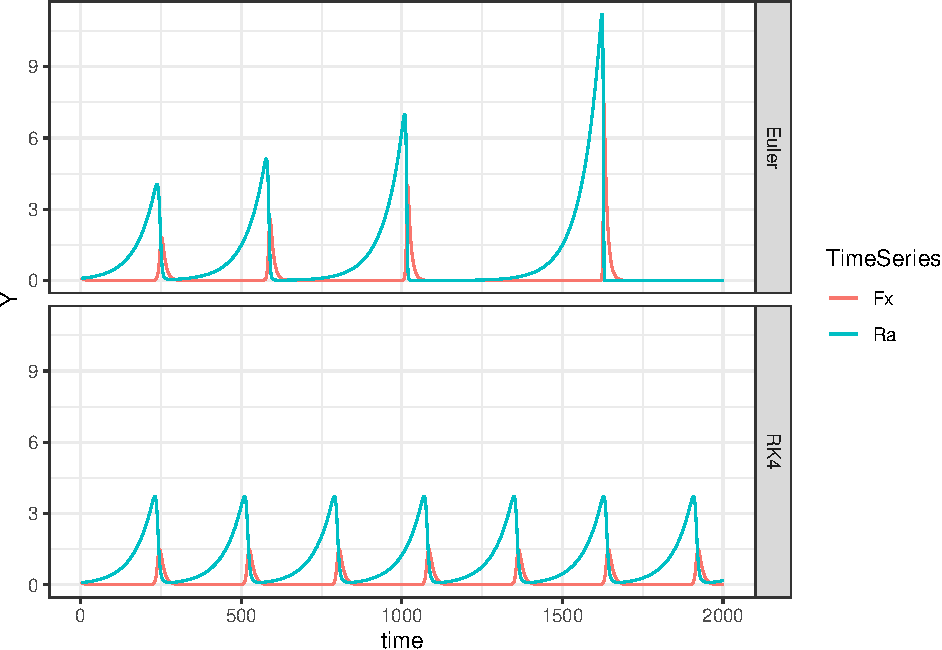
\includegraphics[width=0.99\linewidth]{CSA-Book_files/figure-latex/unnamed-chunk-20-1} \end{center}

\begin{Shaded}
\begin{Highlighting}[]
\CommentTok{# Phase plane plots}
\KeywordTok{ggplot}\NormalTok{(pp, }\KeywordTok{aes}\NormalTok{(}\DataTypeTok{x=}\NormalTok{Ra,}\DataTypeTok{y=}\NormalTok{Fx,}\DataTypeTok{colour=}\NormalTok{time)) }\OperatorTok{+}
\StringTok{  }\KeywordTok{geom_path}\NormalTok{() }\OperatorTok{+}
\StringTok{  }\KeywordTok{facet_grid}\NormalTok{(method}\OperatorTok{~}\NormalTok{.) }\OperatorTok{+}
\StringTok{  }\KeywordTok{xlab}\NormalTok{(}\StringTok{"Rabbits"}\NormalTok{) }\OperatorTok{+}\StringTok{ }\KeywordTok{ylab}\NormalTok{(}\StringTok{"Foxes"}\NormalTok{) }\OperatorTok{+}
\StringTok{  }\KeywordTok{theme_bw}\NormalTok{()}
\end{Highlighting}
\end{Shaded}

\begin{center}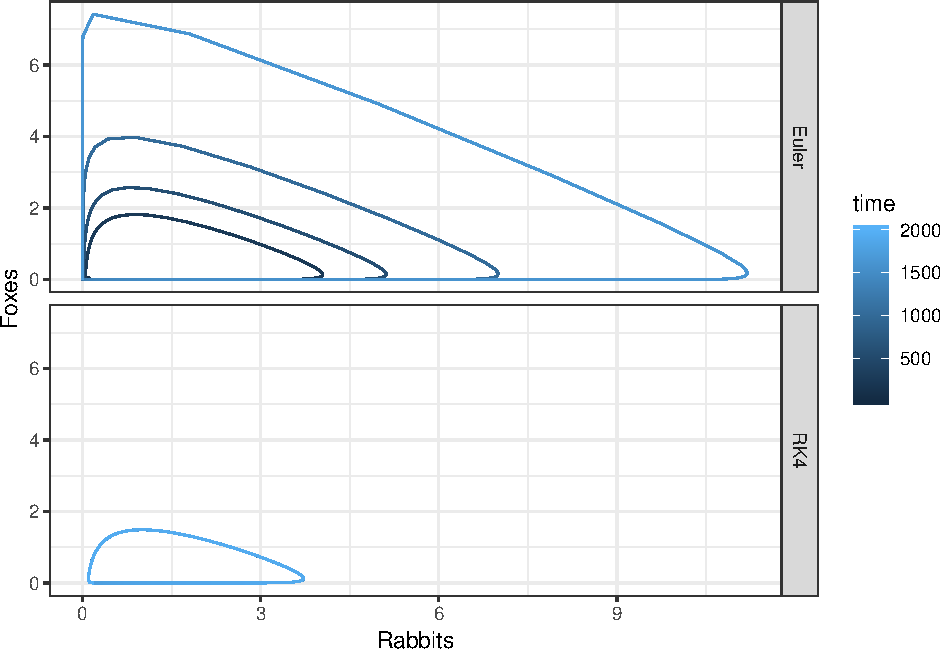
\includegraphics[width=0.99\linewidth]{CSA-Book_files/figure-latex/unnamed-chunk-20-2} \end{center}

Using the Euler method predator and prey populations do not `die out', but in phase space they seem to occupy different behavioural regimes. This looks like an unstable periodic orbit, or an unstable limit cycle, but it is in fact caused by the inaccuarcy of Euler's method. Here \emph{RK4} clearly outperforms \emph{Euler}.

\hypertarget{advmodels}{%
\section{\texorpdfstring{\textbf{Modeling interactions between processes and agents}}{Modeling interactions between processes and agents}}\label{advmodels}}

\hypertarget{the-competetive-lottka-volterra-equations}{%
\subsection{The Competetive Lottka-Volterra Equations}\label{the-competetive-lottka-volterra-equations}}

The coupled predator-prey dynamics in the previous assignment are not a very realistic model of an actual ecological system. Both equations are exponential growth functions, but \textbf{R}abbits for example, also have to eat! One way to increase realism is to consider coupled logistic growth by introducing a carrying capacity.

\begin{itemize}
\tightlist
\item
  Follow the link to the \href{https://en.wikipedia.org/wiki/Competitive_Lotka???Volterra_equations}{Wiki page} and try to model the system!
\end{itemize}

\begin{quote}
This is what \emph{interaction dynamics} refers to, modeling mutual dependiencies using the \texttt{if\ ...\ then} conditional rules isn't really about interaction, or coupling between processes.
\end{quote}

\hypertarget{predator-prey-and-other-dynamics-as-agent-based-models}{%
\subsection{Predator-Prey (and other) dynamics as Agent Based Models}\label{predator-prey-and-other-dynamics-as-agent-based-models}}

Agent-Based models are an expansion of the idea of ``connected growers'' that includes a spatial location of the things that is subject to change over time.

Have a look at some of the \href{http://ccl.northwestern.edu/netlogo/}{NETlogo} demo's:

\begin{itemize}
\tightlist
\item
  \href{http://www.netlogoweb.org/launch\#http://www.netlogoweb.org/assets/modelslib/Sample\%20Models/Biology/Rabbits\%20Grass\%20Weeds.nlogo}{Rabbits Weeds Grass}
\item
  \href{http://www.netlogoweb.org/launch\#http://www.netlogoweb.org/assets/modelslib/Sample\%20Models/Biology/Wolf\%20Sheep\%20Predation.nlogo}{Wolf Sheep Grass}
\end{itemize}

\hypertarget{the-dynamic-field-model}{%
\subsection{The dynamic field model}\label{the-dynamic-field-model}}

Probably the most impressive modelling example in developmental psychology is the Dynamic Field Model for infant perservative reaching, also known as the \emph{A-not-B error}:

\href{https://www.cambridge.org/core/journals/behavioral-and-brain-sciences/article/dynamics-of-embodiment-a-field-theory-of-infant-perseverative-reaching/1C2802AA1C508444DD6D3C3289141CD8\#}{Thelen, E., Schöner, G., Scheier, C., \& Smith, L. (2001). The dynamics of embodiment: A field theory of infant perseverative reaching. Behavioral and Brain Sciences, 24(1), 1-34. doi:10.1017/S0140525X01003910}

The model makes some very interesting predictions that have been confirmed and it has been generalized to other phenomena and scientific disciplines as well

\href{https://www.sciencedirect.com/science/article/pii/S1364661303001566}{Smith, L. B., \& Thelen, E. (2003). Development as a dynamic system. Trends in cognitive sciences, 7(8), 343-348.}

\href{https://www.scribd.com/document/119411540/Using-Dynamic-Field-Theory-to-Rethink-Infant-Habituation}{Schöner, G., \& Thelen, E. (2006). Using dynamic field theory to rethink infant habituation. Psychological review, 113(2), 273.}

\href{http://eprints.lancs.ac.uk/71113/1/Proceedings_final.pdf}{TWOMEY, K. E., \& HORST, J. S. (2014). TESTING A DYNAMIC NEURAL FIELD MODEL OF CHILDREN'S CATEGORY LABELLING. In Computational Models of Cognitive Processes: Proceedings of the 13th Neural Computation and Psychology Workshop (pp.~83-94).}

You can learn about it on the \href{http://www.dynamicfieldtheory.org}{Dynamic Field Theory} website centered around the book:

\href{http://www.oxfordscholarship.com/view/10.1093/acprof:oso/9780199300563.001.0001/acprof-9780199300563}{Schöner, G., \& Spencer, J. (2015). Dynamic thinking: A primer on dynamic field theory. Oxford University Press.}

\begin{center}\rule{0.5\linewidth}{\linethickness}\end{center}

\hypertarget{basic-tsa}{%
\chapter{Basic TSA}\label{basic-tsa}}

\hypertarget{applications}{%
\chapter{Applications}\label{applications}}

Some \emph{significant} applications are demonstrated in this chapter.

\hypertarget{example-one}{%
\section{Example one}\label{example-one}}

\hypertarget{example-two}{%
\section{Example two}\label{example-two}}

Time series of repeatedly measured human performances presents fluctuations around a mean value. These fluctuations are typically considered as insignificant, and attributable to random noise. Over recent decades, it has become increasingly clear that fluctuations in repetitive performance possess interesting properties, however, one of which the property of 1/f, or monofractal, scaling. 1/f scaling indicates that a measured process extends over a wide range of timescales, suggesting that the measured process is assembled over all of these scales simultaneously. The present paper reviews a substantial number of neurological, physiological, and cognitive studies that corroborate the claim that 1/f scaling is most clearly present in healthy, well-coordinated activities. The most prominent hypotheses about the origins of 1/f scaling in human activities are confronted in light of these reviewed studies. A synthesis of this confrontation points towards the conjecture that 1/f scaling in living systems reflects the genuine complex nature of cognitive systems, and casts doubt over claims that 1/f scaling is a coincidental side-effect of information processing sequenced through discrete neurological modules. The consequences of fractal dynamics extending over brain, body and cognition, from the small spatial and temporal scales (e.g., neurons) to the larger scales of human behavior and cognition, are vast, and impact the way in which relevant research questions should be approached. Rather than focusing on specialized isolable subsystems, using additive linear methodologies that specifically aim at doing so, nonlinear dynamics, more elegantly so, imply the more appropriate complex systems methodology, thereby exploiting, rather than rejecting, mathematical concepts that describe large sets of natural phenomena.

The presence of 1/f scaling in human performances is arguably one of the most puzzling, yet lawful phenomena in cognitive science. (see Diniz et al., 2010; Gilden, 2001; Van Orden, Holden \& Turvey, 2003; 2005, Riley \& Turvey, 2002; Slifkin \& Newell, 1998; Wagenmakers, Farrell, \& Ratcliff, 2005). 1/f scaling represents fractal, self-similar processes nested across multiple scales of measurement. Its occurrence implies that the rescaling of a time series leaves the distributional properties of the time series unaffected. Intriguingly from both a statistical and theoretical point of view, fractal scaling is widespread across the central nervous system, motor behavior, cognitive performances, and well beyond. As will be discussed, many physical and physiological signals exhibit scale-invariant features. Because it is now well-known that the presence of 1/f scaling has a profound impact on cognitive and physiological activities, the phenomenon warrants serious attention.

Despite the fact that 1/f scaling is a mathematical concept that allows for descriptions of large sets of natural phenomena, the study of this relatively simple lawful description is relatively new. 1/f scaling, nonetheless, has the potential to reveal unexpected congruities among neurological, physiological and cognitive activities A general back draw is that the observation of 1/f scaling in itself runs against standard statistical intuitions. That is, successive observations of a repeated behaviors are typically assumed to represent measurement values that are independently drawn from a Gaussian distribution, and thus to fluctuate randomly from trial-to-trial. Over recent decades, however, it has become clear that movement variability rarely equates with random, Gaussian noise, and that temporal variability is usually structured and reveals specific details of the system dynamics (Gilden, 2001; Riley \& Turvey, 2002; Slifkin \& Newell, 1998; Stergiou \& Decker, 2011; Torre \& Balasubramaniam, 2011).

In fact, structured variability appears to be the rule rather than the exception, and is often as revealing as aggregate information in terms of unpacking the nature of the system organization (Ihlen \& Vereijken, 2010; Kello, Beltz, Holden, \& Van Orden, 2007; Van Orden et al., 2003).

1/f scaling implies long-range dependence in the signal, often called long-range correlations or long memory. The associated serial correlations from trial to trial decay very slowly as the number of intervening trials increases, indicating persistent serial correlations, in contrast with the traditional view that they are transient (see e.g., Gilden, 2001). This sets 1/f scaling apart from random noise, which lacks this serial dependence.

One way of revealing 1/f scaling is by translating dependencies in the time domain (i.e., a pattern of change in response time over trials) as simple features in the frequency domain using an operation called a Fourier transform, which decomposes the data series containing changes in response over trials into its constituent frequencies. Next, the power (the square of the amplitude) of each contributing wave at that frequency in the decomposed signal is plotted in a log-log power spectrum. Also called power spectral density function, such a log-log power spectrum for a random data series (white noise, see Figure 1a) is shown in Figure 1b.

White noise is not long-range correlated, as represented by a flat slope in a log-log power spectrum. 1/f scaling, in contrast, expresses as an inversely proportional relation between log power and log frequency (see Figure 1d). This implies a nested sequence effect spanning over the entire time course of a measurement and even beyond, encompassing undulating ``waves'' of relatively longer and then shorter response times travelling across the series. Specifically, faster (high-frequent) changes in response time are typically small, and embedded in overarching, slower (lower-frequent) changes of higher amplitude (see Figure 1c). A third class of variability is Brownian noise (see Figure 1e), which can be generated by adding successive observations generated by a white noise process. Brownian noise is nonstationary, which means that variance increases over time. The log-log power spectrum of Brownian noise has a slope of -2 (see Figure 1f).

Figure 1. Three different classes of temporal variability, white noise (a), 1/f scaling (c), and Brownian noise (e), and their respective power spectra are shown in the respective panels at the right.

Typically, repeated human behaviors show a scaling exponent α in the range of 0 and 1, in between random noise and 1/f scaling. Examples of cognitive tasks include mental rotation, lexical decision, and visual search (Gilden, 2001), simple reaction time and word-naming (Van Orden et al., 2003), forearm oscillation (Delignières, Torre, \& Lemoine, 2008), synchronization to a metronome (Chen, Ding, \& Kelso, 1997); implicit associations (Correll, 2008), bi-daily reports of self-esteem (Delignières, Fortes, \& Ninot, 2004), and movement times in an aiming task (Valdez \& Amazeen, 2008; Wijnants et al., 2009), among others. But sometimes α varies between 1 and 2 or even beyond, often in continuous processes like postural sway (e.g., Collins \& De Luca, 1993), force production (Sosnoff, Valantine, \& Newell, 2009), or galvanic skin response (Wijnants, Cox, Hasselman, Bosman, \& Van Orden, 2012).

The aim of this paper is to review the fascinating linkage between 1/f scaling and healthy, well-coordinated activities. Next, the most pertinent hypotheses about the origins of 1/f scaling in human activities are discussed, followed by a critical assessment of their relative strengths and weaknesses. Any of these hypotheses are able to successfully explain the presence of 1/f scaling, but postulate opposing underlying mechanisms. The proposal put forwards is that questions concerning potential mechanisms and models that produce 1/f scaling should be rephrased. What matters is which explanation accounts best for the general linkage between observed fractal dynamics and coordinated physiological and cognitive processes. After all, each distinct accounts will have to deal with this broad linkage.

\begin{enumerate}
\def\labelenumi{\arabic{enumi}.}
\setcounter{enumi}{1}
\tightlist
\item
  Fractal dynamics and system coordination
  Recent years have witnessed increasing empirical support for widespread 1/f scaling in time series of physiological and behavioral processes. A main theme of this review focuses specifically on the association of 1/f scaling with healthy and well-coordinated behaviors. That is, deviations from 1/f scaling are often related to pathologic disorders, aging, external perturbations, high workload, or other situations where the system was not fully functional or coordinated. Rather than an incidental finding, this relation appears to be global, and extends from small spatial and temporal scales (e.g., neurons) to the larger scale of human behavior itself.
\end{enumerate}

That said, the growing body of research has further complicated this picture, showing that changes in the scaling relation occur simultaneously, and sometimes independently, on shorter (i.e., sleep-wake cycles, rest versus exercise, or circadian phases) and longer time scales, such as learning or aging (e.g.~Ivanov et al., 1999; Hu et al., 2004; Kantelhardt, 2002; Karasik et al., 2002; Schumann, Bartsch, Penzel, Ivanov, \& Kantelhardt, 2010). Observing deviations from 1/f scaling in shorter scale processes (e.g., transitions from one physiological state to another) under young and healthy conditions invite for a critical review. of the relation between system performance and the presence of 1/f scaling on the longer behavioral scales, to a) evaluate whether the current state of knowledge allows arriving at a coherent theoretical framework, and b) pinpoint the questions that remain to be answered.

One biological example that hints at the generality of the claimed relation between coordinated system behavior and 1/f scaling are the vibratory motions of the membrane of red blood cells. The human body continuously produces new red blood cells (approx 2.4 million a second, cf.~Sackmann, 1995), which compose a third of the cells in the human body (Pierigè, Serafini, Possi, \& Magnani, 2008). Red blood cells are renewed after approximately 120 days, however. Interestingly, the membrane of red blood cells spontaneously vibrates, or `flickers', revealing 1/f scaling. Costa, Ghiran, Peng, Nicholson-Weller, and Goldberger (2008) in addition that the dynamical properties of this flickering behavior change with in vivo aging. Older cells emit less clear 1/f scaling, compared with newer cells that carry more oxygen.

This example is meaningful, since red blood cells constitute an important, basic system component, which is strongly related to an adequate functioning of one's physiology (and, hence, by extension human behavior). By reviewing functional benefits of fractal dynamics for living systems, an attempt is made to offer a vehicle for theoretical progress on the topic of 1/f scaling in cognitive performances. The steadily growing body of reliable positive evidence contradicts and grossly surprises conventional thinking about the architecture of cognitive systems. For one, a common scale-free `language' among perceptual-motor or cognitive tasks and (neuro-)physiology are not expected from classical componential models, which typically posit domain-specific control structures.

2.1. Pervasive fractal scaling in the central nervous system
Brain activity is being investigated across a multitude of embedded scales of analysis. The finest level is the molecular scale which makes up cells, neurotransmitters etc. Courser levels of brain activity include cell membranes with their synapses, microcircuits of dentritic trees, whole neurons, local cortical circuits consisting out of nearby neurons, entire cortical regions, and interactions among cortical regions and pathways connecting them. At the coarsest scale one finds the central nervous system as a whole, embedded in a body, history, and environment . Evidence of fractal scaling at all of these levels would suggest common dynamical constraints across these embedded scales of organization, begging the question whether the presence of fractal scaling provides support to this multiscale organization.

Anatomically out first, a mammalian brain reveals fractal properties in branching dendrite patterns, thereby maximizing functionality for a fixed dendrite cost (Bassingthwaighte, Liebovitch, \& West, 1994; Kniffki, Pawlak, \& Vahle-Hinz, 1994; Smith, Marks, Lange, Sheriff, \& Neale, 1989), suggesting that fractal scaling in morphological specializations at the cellular level has a functional role (see also Harrison et al., 2002; Milosevic, Ristanovic, Stankovic, \& Gudovic, 2007; Zietsch \& Elston, 2005). As a different example, fractal characteristics of microglia differentiate between healthy and pathological brains (Karperien \& Jelinek, 2008; Soltys, Ziaja, Pawlinski, Setkowicz, \& Janeczko, 2001). And, also at more global organizational levels of the brain, fractal morphology yields functional advantages (Ha et al., 2005, Zhang, 2006).

The spatial fractal structure of brain anatomy aside, temporal dynamics are remiscent of complex behavior across many scales just as well: 1/f power-law scaling in temporal activation patterns has been observed at all levels of neural organization, from ion channels opening and closing times to cortical networks (Werner, 2010). The question of primary interest is how the dynamics of ion channels (Liebovitch \& Krekora, 2002; Liebovitch \& Shehadeh, 2005; Lowen , Cash, Poo, \& Teich, 1997; Takeda, Sakata, \& Matsuoka, 1999, Varanda, Liebovitch, Figueiroa, \& Nogueira, 2000) interact with, rather than concatenate to, fractal spike intervals (Bhattacharya, Edwards, Mamelak, \& Schuman, 2005; Giugliano, Darbon, Arsiero, Luescher, \& Streit, 2004; Grüneis et al., 1993, West \& Deering, 1994), and the functional characteristics of larger scale neural ensemblies (Buzsàki, 2006; Bressler \& Kelso, 2001; Freeman, Holmes, Burke, \& Vanhatalo, 2003; Spasic, Kesic, Kalauzi, \& Saponjic, 2010; Tognoli \& Kelso, 2009; Varela, Lachaux, Rodriguez, \& Martinerie, 2001; Werner, 2007).

Important clues may come from pathological brains. For instance, deviations from 1/f scaling, as typically observed in healthy controls, have been found with major-depressive disorder (Linkenkaer-Hansen et al., 2005), mania (Bahrami, Seyedsadjadi, Babadi, \& Noroozian, 2005), autism (Lai et al., 2010), epilepsy (Ramon, Holmes, Freeman, McElroy, \& Rezyanian, 2008), and Alzheimer's disease (Abásolo, Hornero, Gómez, García, \& López, 2008). These results suggest that 1/f scaling is prevalent in healthy, coordinative behavior of a healthy brain, and less so in the global activity of the brain with disorders and disease. Following on this suggestion, it was shown that the presence of 1/f scaling in brain activation correlates with the severity of depression symptoms (Linkenkaer-Hansen et al., 2005) and the success rate of recovery from traumatic brain injury (Burr, Kirkness, \& Mitchell, 2008).

The scale complexity inherent to the study of brain activity makes it an enormous challenge for neuroscience to arrive at a universal theory of brain function. One first complication comes from the requirement of different methods at each level or scale of neural investigation. Each of the methods available yields a compromise between spatial and temporal resolution and, consequently, yields a priori choices in the organizational level of interest. No current method in isolation is likely capable of revealing the full-blown complexity of the brain, from the decimeter to the micrometer scale and from milliseconds to minutes up to developmental timescales. The discussed findings, however, should be taken as a strong suggestion that the inherent scale complexity of the human brain is a (if not the) key feature in itself.

2.2. Pervasive fractal scaling in the body
A substantial amount of fractal applications in cognitive research have been motivated by initial successes in physiology, which had related 1/f scaling to the coordination, adaptivity and flexible stability of the involved regulatory processes. Deviations from 1/f scaling in physiology have been found to relate to the degradation and decoupling of integrated systems, pathological conditions, severe disease and increased mortality risk.

For instance, heartbeat interval series show 1/f scaling, with the clearest examples in healthy subjects. Deviations from 1/f scaling, either associated with excessive order (pathologic periodicity), or uncorrelated white noise (lack of temporal organization), indicate pathological conditions like congestive heart failure and ventricular arrhythmia (Goldberger, 1997; Peng et al., 1995), and thus predict mortality (Mäkikallio et al., 2001). Smaller deviations from 1/f scaling have been observed in heartbeat intervals in obese children (Vanderlei, Pastre, Júnior, \& de Godoy, 2010) and adults with Down Syndrome (Mendonca, Pereira, \& Fernhall, 2011).

However, although alterations in the fractal properties of physiologic signals have been found to be reliable markers of changes in physiologic control, with healthy aging scale-invariant and nonlinear properties of heartbeat dynamics remain unchanged, with heart rate variability is significantly reduced healthy elderly, nonetheless (Schmitt \& Ivanov, 2007; Schmitt, Stein, \& Ivanov, 2009). These findings suggest that healthy aging may not result in a continuous gradual change in scaling properties of heartbeat intervals, and implies that alterations in the cardiac control mechanism with advanced age differ conceptually from the mechanistic changes in the autonomic regulation associated with pathologic conditions.

Also breathing rhythm reveals 1/f scaling behavior, but shows deviations thereof with aging (Peng et al., 2002; West, 2006). The contrary goes for development. Fetal breathing movements show more pronounced 1/f scaling with gestational age (Govindan, Wilson, Murphy, Russel, \& Lowery, 2007). In contrast, deviations from 1/f scaling are observed in asthma patients, out of which those with more pronounced 1/f signatures in breathing rhythm showed better recovery after treatment (Frey et al., 2005). These findings indicate together that fractal dynamics increase the overall efficiency of the respiratory system (cf.~West, 2010).

Also fluctuations in blood pressure are found to scale as 1/f (Mutch et al., 2000, Brogan et al., 2007). Diabetic patients, however, show reduced 1/f noise specifically in glucose fluctuations compared with healthy controls (Ogata et al., 2007; Yamamoto et al., 2010). Other examples include by fluctuations in colonic pressure. Yan, Yan, Zhang \& Wang (2008) observed 1/f fluctuations in the colonic activity of the healthy subjects, while patients hospitalized for slow transit constipation showed colon pressure fluctuations deviating from 1/f noise towards Brownian noise; a condition yielding hardly bearable levels of pain sensation.

In physiology and medicine it is being increasingly acknowledged that a disease not only changes an average measure, such as heart rate or breathing rate, but is manifest in departures from fractal variability. Deviations from 1/f scaling are taken to imply a loss of physiologic control, which is often visible at very early stages of pathological development. The change in fractal dynamics with disease and, in some cases, aging suggested the new definition of disease as a loss of complexity, rather than the loss of regularity (e.g., Goldberger et al, 2002).

2.3. Pervasive fractal scaling in motor control
As in neuroscience, medicine, and physiology, there has been an increasing interest in fractal dynamics in human movement science. For instance, time series of postural sway differ reliably from random noise, revealing fractal properties (e.g., Duarte \& Sternad, 2008; Duarte \& Zatsiorsky, 2001; Collins \& De Luca, 1993). Moreover, the clearest examples of 1/f scaling are found in young participants, while elderly participants show less clear fractal scaling in their postural dynamics (Doyle, Dugan, Humphries, \& Newton, 2004), indicating degraded balance control (Collins \& De Luca, 1995; Laughton et al., 2003; Maurer, Mergner, \& Peterka, 2004; Priplata, Niemi, Harry, Lipsitz, \& Collins, 2003; Priplata et al., 2006). This interpretation was further supported by Manabe et al. (2001), who demonstrated less clear 1/f scaling in postural sway dynamics for patients suffering from Parkinson's disease and spinocerebellar ataxia, when compared to a control group. Interestingly, fractal measures of postural sway were even found more reliable than more traditional measures (Doyle, Newton, \& Burnett, 2005).

Also in gait intervals (Hausdorff, 2007; 2009, are reviews), - the time intervals between successive steps in locomotion -, the clearest examples of 1/f scaling are observed in young and healthy participants, whereas with aging, gait interval series become more random. It must be noted, however, that, while cardiac and respiratory dynamics show a more pronounced 1/f scaling and also higher degree of nonlinearity with gestation age and maturation, locomotion exhibits deviations from 1/f scaling towards more random scaling are observed as early as maturation from childhood to adulthood (cf.~Ashkenazy, Hausdorff, Ivanov, Goldberger, \& Stanley, 2008; Hausdorff et al., 2001).

In an elderly population, however, the presence of 1/f scaling successfully discriminates between fallers from non-fallers, and between Huntington's patients and control participants (Hausdorff, 2007). Moreover, the fractal dynamics of stride intervals produced by Huntington's patients correlates strongly with the severity of the illness (r = -.78, cf.~Hausdorff, 2007), suggesting that deviations from 1/f scaling suggest impaired control of locomotion. Hausdorff (2009) describes similar findings in Parkinson's disease patients, and observed that among patients Parkinson's disease, the 1/f scaling relation in gait intervals ``breaks down'' and the stride-to-stride fluctuation in gait becomes very similar to white noise; each stride starts a new process, unlinked and unrelated to the previous stride. After successful treatment with proper medication, however, 1/f scaling becomes more prominent again in Parkinson patients' gait dynamics (Auriel, Hausdorff, Herman, Simon, \& Giladi, 2006).

Using a different motor task, Wijnants, Bosman, Hasselman, Cox, and Van Orden (2009) presented college students with a very challenging precision-aiming (i.e., Fitts) task. The instruction was to move as fast and as accurately as possible between two circular targets with an inkless stylus. Participants were presented with five training blocks of 1100 back-and-forth movements. Very small targets were used, positioned wide apart, while participants were instructed to use their non-dominant, least-practiced hand. A learning effect was observed after the extensive number of practice trials. Participants reached the narrow targets much faster after practice, while accuracy was maintained. A reliable effect of practice was found in the presence of 1/f scaling in movement time fluctuations; the presence of 1/f scaling became more pronounced with motor learning.

In a later study, Wijnants, Cox, Hasselman, Bosman, and Van Orden (2012) examined 1/f scaling in both spatial (movement amplitude) and temporal (movement time) time series in the challenging precision-aiming task, so notorious for revealing speed-accuracy trade-off (cf.~Fitts, 1954). Because of the difficulty of the task, participants were required to either emphasize the speed or the accuracy side of the trade-off (while equally being instructed to move as fast and as accurately as possible between targets) simply because the dual task constraints were so incompatible. The emphasized task requirement (temporal or spatial) directly affected the presence of 1/f scaling. Faster participants produced clearer 1/f scaling in movement times, but more random dynamics in movement amplitudes, as they performed the task less accurately. Conversely, more accurate participants produced more random dynamics in movement time sequences, as they performed the task more slowly, and clearer 1/f scaling in movement amplitude series. This effectively led to a trade-off between spatial and temporal 1/f scaling (ρ = −0.64), contingent on the so well-established speed-accuracy trade-off.

In the same study, Wijnants et al. (2012) established a strong relation between the fractal dynamics of movement time vs.~movement amplitude and the biomechanical constraint of minimizing the dissipation of mechanical energy. Faster participants, who produced clearer 1/f scaling in their movement time series also better capitalized on the elastic properties of the muscular system to recycle the kinetic energy of the approaching hand, arm, and shoulder in potential form, which is energetically to the benefit of the next movement. Together, this amounted to a strong coupling among measurement scales in human performance: the biomechanical details emerged within the timeframe of a single movement, while speed and accuracy are determined by entire movements. The third timescale included the fractal dynamics that extend up to minutes of performance. The strong coupling between these multiple levels of motor performance provided further exquisite support for the nested multi-scale properties in the organization of the cognitive system.

In contrast, externally driven performances have been found to minimize intrinsic fractal fluctuations. For instance, Chen, Ding, and Kelso (1997) observed no 1/f scaling when tapping to a metronome (1/f scaling was observed in the asynchronies to the metronome, nonetheless), while 1/f scaling is clearly present in self-paced inter-tap intervals (cf.~Gilden et al., 1995). Similarly, in consecutive gait-cycles the external drive of a metronome breaks down the long-time correlations of the natural pace and generates random variability (Hausdorff, 2007).

In a bimanual force production task, Wing, Daffertshofer, and Pressing (2004) observed random or close to random variability when feedback was presented to the participants (another form of external drive), while much clearer 1/f scaling was observed when no feedback was provided. Kello et al. (2007) and Van Orden et al. (2003) interpreted these findings, altogether, as a confirmation that feedback provided constitutes a type of external perturbation that de-correlates the intrinsic fluctuations of 1/f scaling.

Perhaps the epitome of exercising external perturbation to motor control is to add a cognitive task on top of an initially simple motor task. Dual-tasking paradigm has been found to induce reduced 1/f scaling in the primary motor task (Kiefer, Riley, Shockley, Villard, \& Van Orden, 2009). This finding was replicated in a different task by Hausdorff (2009); who Parkinson's patients to walk while performing a challenging secondary task. The gait dynamics revealed a reduced presence of 1/f scaling, compared with a no dual-tasking condition.

2.4. Pervasive fractal scaling in human cognition
The presented results from neuroscience, physiology, and movement science, naturally extend to cognitive performances. Consider Figure 2, which depicts the average 1/f scaling exponents observed in four different experiments; word naming (Van Orden et al., 2003), choice reaction (Kello et al., 2007), simple reaction (Van Orden et al., 2003), and precision aiming (Wijnants et al., 2009). It is clear that the presence of 1/f scaling gradually increases over these tasks. Note that in precision aiming and simple reaction tasks, each experimental trial is identical. Each trial yields the same stimuli and the same type of response. This means that external sources of variation are minimized in these task performances. Consequently, the observed variation must largely reflect internal sources, which can be seen as a clearer presence of 1/f scaling in those tasks. One can readily notice the difference between precision aiming and simple reaction times. Precision aiming is a cyclic task, while simple reaction times become perturbed by a discrete signal to respond at each trial, and requires a discrete response at each trial. It can be seen that the extent of this perturbation effectively leads to a reduced presence of 1/f scaling.

The other end of the scale shows the 1/f scaling exponents from a word-naming task and a choice reaction task. In these tasks, each experimental trial differs, but to a different extent. In the choice reaction task, four different signals to respond were presented, with each signal requiring a different response. This procedure introduces more external sources of variation, which is revealed by a more whitened 1/f signal. Word-naming reveals the most reduced example, a task in which every experimental trial introduces a unique signal to respond. Hence, external sources of variation are maximized in this procedure, and the measured values likely reflect the intrinsic sources of variation to a lesser extent, requiring a more flexible and adaptive, perhaps less organized, control strategy. Similarly, the presence of 1/f scaling is typically reduced under high workload conditions (Clayton \& Frey, 1997; Correll, 2008; 2011) and when a sequence of presented stimuli becomes less predictable (Kello et al., 2007).

Figure 2. The fractal scaling exponents from four independent experiments are shown. It is shown that 1/f scaling become more clearly present as the number of different response options decreases (see text). The shown tasks include word-naming, choice reaction, simple reaction, and precision aiming.

A closer look at one of the tasks, choice reaction, reveals a similarly interesting finding. Ward (2002) discusses an experiment that was set up to manipulate the number of stimulus and response alternatives. In that study, Ward and Richard (2001) presented participants with a choice reaction task that consisted out of either one (simple reaction), two, or four stimulus-response alternatives. The authors effectively showed that the presence of 1/f scaling is reduced as the number of stimulus-response alternatives increased. The scaling exponents were .60 for the simple reaction task, .37 for the two- choice reaction task, and .24 for the four-choice reaction task ..

Another example of systematic perturbations attenuating the presence of fractal dynamics comes from Kuznetsov and Wallot (2011), who presented participants with a temporal estimation task, in either of five conditions of accuracy feedback. In one condition, feedback was provided at every estimate, in another condition no feedback was given at all. In the remaining conditions, feedback was displayed only if the temporal estimate deviated from the target interval by more than 50, 100, or 200 ms respectively. The results revealed an increase of 1/f scaling in conditions where less feedback (i.e., intermittent sources of perturbation) was provided, and hence, where the intrinsic cognitive fluctuations were revealed most clearly.

Gilden and Hancock (2007) compared the performance of adults who reported Attention Deficit Hyperactivity Disorder (ADHD) symptoms with a control group of adults who did not, in a mental rotation task. The instruction was to press a key if the stimulus (a letter rotated by 0, 60, 120, 180, 240, or 300 degrees) was mirror-inverted, and another key if the stimulus was not. Distinctive dynamical patterns of response in the reaction times were observed in both groups. More consistent participants revealed fractal scaling exponents close to 1/f scaling, while the more variably performers revealed random walk dynamics with a spectral slope close to -2. Hence, the more efficient system responses yielded a relatively clear 1/f signal, while the less coordinated, attention-deficit responses deviated from that pattern.

Wijnants, Hasselman, Bosman, Cox, \& Van Orden (2012) inquired fractal scaling properties in the context of another learning disability. Response latencies of young children diagnosed with developmental dyslexia were compared with response latencies of non-dyslexic children. The authors revealed that 1/f scaling measures reliably differentiated between both groups of readers when reading aloud single words sequentially. The dyslexic readers revealed more random response times, while average readers revealed clearer 1/f scaling. Furthermore, in the dyslexic group the 1/f scaling exponents of the response time series strongly correlated with the severity of the reading impairment, as determined by average response time (r = -0.56, the negative correlation indicates that slower responses were associated with less clear 1/f scaling) and standardized reading scores (r = 0.77, the positive correlation indicates that lower reading scores are associated with less clear 1/f scaling).

The summarized findings from research incorporating behavioral responses to repeated stimuli are very similar to the findings in neuroscience, physiology and movement science. These findings raise the suggestion that many measurements related to how humans respond to repeated stimuli reveal signatures of complexity akin to the scaling behavior observed in simultaneously occurring processes (e.g., in the brain and the body). Importantly, these `cognitive' processes are traditionally treated as independent and self-supporting `directive systems' (i.e., the brain modules `in charge') or `executive systems' (i.e., the autonomous nervous system `doing what it is directed to do'). The very observation that they may not be independent and self-supporting, but rather massively interactive, -- and complex in a true complex systems sense- , could however, cast doubt on the validity of the common sense distinction between the directive and executive front seemingly involved in the coordination of human action (Van Orden, Hollis, \& Wallot, 2012; Varela et al.~2001).

\begin{enumerate}
\def\labelenumi{\arabic{enumi}.}
\setcounter{enumi}{2}
\tightlist
\item
  Theoretical perspectives on 1/f scaling in human performance
  1/f scaling relations are systematically manipulable, and indicate adaptive and flexible performances where no single timescale dominates coordination. Cognitive systems thus appear to ongoingly maintain a balance between competitive and cooperative processes in a flexible coupling across brain, body and cognition. By confronting the most prominent, yet competing, hypotheses with the empirical observations presented above, an attempt is made towards a single conclusive theoretical account.
\end{enumerate}

3.1. Multi-scaled randomness
One account for widespread 1/f scaling in human cognition conceives the phenomenon as reflecting many independent processes, each acting individually on their own timescale (e.g., Granger, 1980; Hausdorff \& Peng, 1996; Pressing, 1999; Wagenmakers, Farell, \& Ratcliff, 2004; Ward, 2002; Wing et al., 2004). For example, consider a time series where each measured response X constitutes the sum of three different processes Y1, Y2 and Y3, each evolving at their own independent timescale, in the additive form; X(t) = Y1(t) + Y2(t) + Y3(t). If one then assumes that Y1 is a quickly random changing process, Y2 is a random intermediate process, and Y3 is a slowly randomly changing process, the additive series of all Y's may yield 1/f scaling under specific circumstances (see for instance, Hausdorff \& Peng, 1996; Wagenmakers et al., 2004).

Figure 3 shows schematically a power spectrum from repeated responses that combine the activity of a multitude of independent processes, each at their own timescale. In this schematic representation, indeed, the schematic distributions of time scales lead to 1/f behavior (see e.g.~Beran, 1994, for a more detailed description). This suggests that the complex fluctuations and 1/f scaling observed in many biological systems do not convey anything `special' about the mechanism generating these dynamics. From this perspective, 1/f scaling is a rather coincidental event that reflects nothing more than an artifact of information processing.

Figure 3. A schematic representation of the multi-scaled randomness construct. The left panel shows five hypothesized processes, each evolving at their own timescale. A time series composed of the sum of these processes may reveal 1/f-like noise in a power spectrum, which is shown in the right panel. Note that the processes are depicted schematically, and may compose random processes with differing relaxation times, rather than deterministic sine waves.

The main benefit of explaining 1/f scaling by aggregation of component processes is that such an explanation is conceptually simple and seemingly transparent, and may therefore `demystify' the widespread occurrence of 1/f scaling (cf.~Wagenmakers et al., 2004). That is, a componential model, consisting of many independent components, is effectively able to produce transient short-range correlations that, together, by chance may closely mimic the 1/f scaling behavior that is so ubiquitously observed across neurology, physiology, motor behavior, and cognition (e.g., Hausdorff \& Peng, 1996; Pressing, 1999; Wagenmakers et al., 2004; 2005).

Consider for instance the often cited dice-throwing algorithm in Gardner (1978). When from three dice, the first is thrown only rarely, the second intermittently, and the third at every observation. The sum of the values, when taken over a range of observations, will fluctuate in a 1/f-like fashion, under specifically constrained conditions.

Nonetheless, there are a number of drawbacks. For one, independent multi-scaled processes must exactly match the power and frequency associated with each involved component in order to coincide with a 1/f scaling pattern. However, if all parameters of the model are free, it is very unlikely that a system would, by chance, choose the ``proper'' parameters necessary to consistently generate 1/f-like noise, let alone accumulate consistent relative changes across so many manipulations in neuroscience, physiology, and cognitive science. That is, ``simulations demonstrate that if model parameters are unconstrained, the likelihood of generating 1/f noise is quite small. Thus, while the model can be used to generate 1/f noise with various scaling exponents, it is unlikely that the 1/f behavior observed in many biological systems is due only to the fact that these systems are regulated by many different inputs acting on different time scales.'' (Hausdorff \& Peng, 1996, p.~2154).

A second important drawback from multi-scaled randomness is the lack of parsimony in the model. For every independent 1/f signal observed new components need to be asserted (Kello et al., 2007; Kello, Anderson, Holden, \& Van Orden, 2008; Van Orden et al., 2003; 2005). If not, that would mean the components are shared between processes, meaning each component is notstrictly interdependent. Components of perception and action would hinge on synergies of physiological and cognitive component activities.

If one, in addition, considers a non-generic 1/f process measured over a time range of ten minutes, or twenty minutes, regardless of its nature, multi-scaled randomness woul imply scaling relations to bend off at the lowest frequencies in the log-log power spectrum when sampling extends over longer periods of time (e.g.~Pressing \& Jolley-Rogers, 1997). In the counter case, infinitely more short-range processes are to be invoked to keep the spectrum from flattening at the low frequencies (e.g.~Torre \& Wagenmakers, 2009; see Van Orden et al., 2005), which woul not be very parsimonious. Surely, the scaling relation may break down at extreme sides of the spectrum, but the criterion held in physics, which is observing 1/f scaling over at least two decades of frequencies, is generally well met in cognitive performances.

Thirdly, notwithstanding that the idea of identifying processes at different time scales is interesting and seems viable, the theoretical interpretation of the different time scales, and the identification of their source still remains quite speculative. That is, the theoretical underpinnings for how and why exactly the hypothesized processes fluctuate in that specific manner are often underspecified in multi-scaled randomness approaches. The critical question is not whether multiple independent processes could cause 1/f scaling in a measured signal (cf.~Wagenmakers et al., 2004; 2005), but rather the specific manner in which those processes must fluctuate. In particular, for any observed 1/f time series, which are many, one needs to examine the number of reasonable time scales involved in the specific process, the approximate values for those time scales, and the relative magnitudes of each influence. The involved processes that evolve at distinct timescales may themselves be as general as corresponding to conscious, preconscious processes, and unconscious processes (Ward, 2002), neural, behavioral and cognitive events (Pressing, 1999), planning and control (Valdez \& Amazeen, 2008), or automatic, conscious, and sustained attention (Wagenmakers et al., 2004).

Despite the simplicity of the model itself, the examination of the data is limited to post-hoc accounts for how neural, behavioral and cognitive events, attentional processes, or consciousness components are supposed to overlap (see Torre \& Wagenmakers, 2009; Van Orden et al., 2005).

When confronted with the experimental results reviewed above, revealing consistent changes in scaling exponent in different performances, from the fastest neural scales down to the slower behavioral processes, the `demystifying' multi-scaled randomness approach of 1/f in human cognition, in fact, becomes an extraordinary hypothesis in itself. That is, the assumption that the observed behavior is jointly determined by many independent groups of neurons, each with their own different relaxation rate (determined by an autoregressive decay parameter) carries a massive theoretical load. The challenge would be to seek for deficient system components in depression symptoms, retiring red blood cells, as well as in severe constipation, asthma, dyslexia or heart failure, among the many other examples, all happening to line up as a reduced 1/f signature.

3.2 Regime switching
A second perspective on 1/f scaling in human cognition assumes that response processes show discrete transitions from one mode of operation (i.e., a specific mean or variance) to the next. These so-called regime switching models propose that shifts in the mean or the variance of the observed process express shifts in strategy, fatigue or attention. First, it is assumed that, over the course of an experiment, participants repeatedly change strategies. These shifts are employed for only a limited period of time each. During these periods, particular threshold levels determine the criterion amount of accumulation of information required for a response. These changing threshold criteria present themselves as different plateau-like variations (see top panel in Figure 4). Secondly, the speed with which the accumulation process approaches the current threshold is assumed to vary between successive measurements as a first- (or sometimes higher) order autoregressive process (see middle panel in Figure 4).

Under well-specified parameterizations regime-switching models are able to effectively generate 1/f-like fluctuations (e.g., Wagenmakers et al., 2004; 2005), as shown in the lower panel of Figure 4. Regime-switching models may also account for non-stationarity (i.e., large criterium switches) and sudden switches in performance mode. Cognitive experiments designed to measure the degree of 1/f scaling are generally lengthy, as they usually require 29, 210, or more trials. In those experimental set-ups measured values are sometimes indeed susceptible to undesired effects of learning, fatigue, shifts in strategy and attention, and the like. This means that it is well possible that many short-range dependencies happen to line up as 1/f scaling, showing ``that 1/f noise is by no means ubiquitous in psychology'' (Farrell, Wagenmakers, \& Ratcliff, 2006, p.~740). Specifically, `something that looks like' 1/f scaling may simply cause a coincidental by-product of cognition through fluctuations in fatigue, attention or strategy.

Figure 4. The top panel represents the plateaus induced by the discrete regime switches. The middle panel represents the autoregressive response variability that is inserted to the model. The response series shown in the lower panel was created by dividing the threshold criterion (top panel) by the information accrual time (middle panel), cf.~Wagenmakers et al. (2004).

It is admittedly mysterious then, that 1/f scaling is so genuinely observed across across the broadness of time scales of neurology, physiology, motor behavior and cognition, simultaneously. Adding the coincidences (as it applies to independent events in probability theory) associated with the discussed studies underscores that the critical question is not whether strategy, attention, or fatigue fluctuations cause 1/f scaling, but rather the specific manner in which the component activities must fluctuate to cause exactly 1/f scaling, and its variations in the face of experimental manipulation. The associated coincidence renders regime-switching models as poor theoretically viable candidates to account for 1/f scaling in human cognition, lacking any physical motivation.

In addition, one could consider the fact that the broad family of autoregressive moving-average models can reproduce exactly any spectral function after the fact, as long as the spectrum has an asymptotic white region at low frequencies, because the model family has so many free parameters. A first inconvenience, as mentioned before, is that in psychological data the low frequency region does not bend off, suggesting genuine long-range dependence.

Secondly, the revealance of reduced 1/f scaling in repeated cognitive performances in some of Wagenmakers et al.'s experiments, which would indeed be expected given the postulated multifarious origins, could be explained by the random inter-trial intervals used in these experiments, which was later shown to disrupt scaling (see Holden, Choi, Amazeen, Van Orden, 2011).

Third, the apparent success of the model is determined by goodness-of-fit per se, and again, realistic data can only be described by a rather narrow set of possible parameter variation (see Gilden, 2009). The question is thus whether a model is a true representation of psychological processes or whether the model itself is so flexible that it is simply able to bend with the measurement error in producing good scores on goodness-of-fit. As Gilden (2009) notes: ``Regardless of how small the minimum chi-square is for a particular set of parameter values, one will eventually have to reckon with the fact that the model did not predict that specific outcome; it predicted a range of outcomes, one of which may have happened to look like the data.''.

Wagenmakers and colleagues claim that their componential models are ``specified in enough detail to allow a wide range of data to be successfully described and, more important for scientific rigor, predicted'' (Wagenmakers et al., 2005, p.~114). The first part of the sentence (i.e., the descriptive part) is obviously true, but disappointedly has little to do with the second part (i.e., prediction). As aptly summarized by Gilden, Wagenmakers et al.'s approach describes so much, it in turn explains very little, and only offers a vehicle for mathematical formalism aimed at post-hoc data fitting, lacking a supporting theoretical literature. Therefore, the theoretical predictions mentioned in the second part of the sentence remain unclear. How do the ARMA model parameters corroborate and predict such consistent changes in the presence of 1/f scaling across such a variety of experimental manipulations? What is the theoretical ground for exactly the fitted parameters? Why is 1/f scaling so allied with coordination in complex systems, being only an artifact? The requisite list of post-hoc explanations required to dismiss 1/f scaling as being functional, across all scales of observation, from the neuron up on to behavior itself, is simply too long, rendering the regime-switching model a rather speculative hypothesis.

3.3 A blend of short and long range correlations
A second prominent theory about 1/f scaling in human performance is the two-source model (Gilden 1997; 2001; 2009; Gilden et al., 1995; Thornton \& Gilden, 2005). This model is motivated by the fact that a log-log power spectrum often does not exactly follow a straight line, and may reveal a flattened (hence, whitened) slope at the highest frequencies.

The high and low-frequency range can thus be modeled in terms of a constrained mixture of two distinct families of variability; white noise and 1/f scaling. These blended sources of variability are referred to as fBmW, where fBm stand for fractional Brownian motion and W for whitened, to emphasize the hybrid structure of whitened 1/f noises.

A fBmW response series has following form: RTn = (1/f α)n + β N(0,1), where RTn is \ldots{}, (1/f α)n is the nth data point in a 1/f signal with zero mean and unit variance, and N(0,1) denotes a random sample from the normal distribution with zero mean and unit variance. β denotes a free parameter that determines the relative contributions of the white noise component. Accordingly, the power spectrum is built from the correlated and uncorrelated parts in a fBmW signal: S( f ) = N(α) f α + β2, where β2 is the fraction of variance in the random process attributable solely to white noise (see Figure 5).

Figure 5. The top left panel shows a white noise signal, which was added to the 1/f scaling in the lower left panel to construct the power spectrum in the right panel, which reveals fBmW noise, as indicated by the flattened slope at the highest frequencies, shown as a solid line. The dashed line represents the ideal 1/f scaling slope.

A difference between Gilden et al.'s account and the two models previously described is that 1/f scaling is conceived of as residing from a functional part of the cognitive system, rather than as a statistical artifact. In the approach of Gilden and colleagues, the presence of 1/f scaling represents a genuine fractal process, indicating that cognitive processes are complex across multiple temporal scales. A natural prediction is that 1/f scaling is generic to the behavior of cognitive systems, and an intrinsic property of the system.

At the other hand one could note that 1/f scaling is not exactly seen as a dynamical signature of an entirely integrated system either. 1/f scaling is rather hypothesized to reflect the self-organization of a component within the system, a component that is associated with elementary aspects of cognition, including the goals, intentions, and representations of a participant. Specifically, Gilden (2001) postulated that intrinsic fluctuations of a memory module, which serves the purpose of continuity of `mental set', are potentially causal in the formation of 1/f scaling. Other processes, e.g.~motor processes, constitute a source of contaminating white noise, and human performances constitute an additive blend of a complex 1/f process and the pure white noise signal, in varying degrees in different performances.

The two-source approach fits in with more traditional models, where cognitivist dual system models are common. The mental set hypothesis may explain why the presence of 1/f scaling is reduced in cognitive performances when the task is not constant across trials. For instance, when task parameters change unpredictably, mental set is interrupted, which will induce trial independence in responses, resulting in scaling properties closer to white noise. An example given by Gilden (2001) is task switching. This interpretation appears viable if one considers the varying degree of 1/f scaling in the four tasks presented in Figure 2. Specifically, Thornton and Gilden (2005) presented a detailed account for Figure 2 based on their model, by showing that temporal estimation tasks (comparable with the precision aiming task in Figure 2 for the present purpose) not only reveals clear 1/f scaling, but also a contribution of the white noise component, while a choice reaction task shows less clear 1/f scaling, with a much stronger white noise contribution, and word-naming data reveal the least clear presence of 1/f scaling, and the strongest contribution of white noise. It thus appears that the model adequately describes a subset of the discussed data.

Nonetheless, the model does not specify specifically which of the dual components in the model would change specifically, and specifically why or how the error term gives complementary information. The presented results also suggest that an independent system component attributed to mental set (Gilden, 2001) or vigilance (Gilden \& Hancock, 2007) might be too limited in scope to account for all shared instances between 1/f scaling and coordination in brain, body and behavior, across the measurement scales involved.

A related approach to 1/f scaling originates from Delignières and colleagues, and has been applied primarily to rhythmical movements. These authors have presented a series of concrete models, each specific to a well-defined domain of motor performance, that effectively mimic empirically observed scaling properties. Like Gilden, their approach is to insert a local source of 1/f scaling in statistically well-defined, local parts of traditional cognitive models, to account for the relative presence of 1/f scaling and specific spectral deviations thereof. As an example, Delignieres, Torre, and Lemoine (2008) adapted the Wing-Kristofferson model (1973) for finger tapping, by inserting fractal properties, into the cognitive timekeeper module assumed by the traditional model, using the regime-switching model previously discussed. Their model accounted for the scaling properties of self-paced tapping. Other examples include synchronized tapping (Torre \& Delignières, 2008a), and forearm oscillations (Delignières et al., 2008).

Delignières et al.~point out that their purpose is to account for the workings of a particular, domain-specific component encapsulated in the system, and use 1/f noise as a constraint for modeling. Sources of 1/f scaling are taken to represent complex timekeeping processes that can be statistically localized in components within the system. Thus from this perspective, 1/f scaling represents a functional aspect of human performance related to cognitive timekeeping, but the different source of 1/f scaling in each domain-specific application has the form of a fractal generator that, together with non-fractal components, makes up the dynamics of repeated responses.

Mechanistic (i.e., two-source) modeling has the advantage to be experimentally testable and thus falsifiable, and allows establishing links to current models of sensorimotor behavior. There is no a priori reason why long-range and short-range dependence should be mutually exclusive (cf.~Van Orden et al., 2005; Wagenmakers et al., 2005), and thus the observed serial correlations are possibly the result of both, and mechanistic models provide a route to separate the long-range from the short-range components. Separation of variance components led to good fits to empirical data in specific tasks, under the assumption that different system components are responsible for the differences in performance (e.g., Delignières \& Torre, 2011).

Interestingly, the timekeeping hypothesis proposed by Delignières and colleagues appears to be consistent with the lack in 1/f scaling when participants synchronize to a metronome (i.e., an external timekeeper) evidenced in tapping and walking experiments as discussed previously.

The concern, again, is the approach of post-hoc data fitting. While good data fits may be compelling, agreement between model and data is not proof that the model is correct (cf.~Gilden, 2009). The pitfall of mechanistic modeling is that one may mistakenly believe that a good quantitative model fit equals qualitative or theoretical insight. A good fit to the data is a necessary, but not a sufficient criterion for a model's usefulness (Roberts \& Pashler, 2000). A consideration of a model's usefulness involves, for instance, also a consideration of the theoretical foundations, the extent to which the model points to new research directions, and the generalizability of the model.

Advanced data fitting may lead to an indefinite number of fractal generators throughout brain, body and cognition, possibly leading to multiple competing models capable of equally compelling fits to the data (Gilden, 2009; Hasselman, Seevinck, \& Cox, 2011), which would question in itself the tenability of domain-specific theoretical explanations of 1/f scaling (Kello et al., 2007). Specifically, a full account for the reviewed studies would require domain-specific models for each of the observations across scientific domains, and scales of observation. Although this could arguably lead to a well-fitting model for each separate phenomenon, that approach would lack the coherence of a solid theoretical framework over brain, body and cognition necessitated.

3.4 Interaction-dominant dynamics
1/f scaling is a typical behavior of self-organizing systems, which reflects a fundamental aspect of all physiological and cognitive functions: their emergence in the balance of independent versus interdependent component activities. Interaction-dominance postulates that the cognitive system actually uses this ``flexible stability'' to its own advantage by exploiting the interdependencies among ongoing processes over a multiplicity of interdependent scales, allowing for a coordinative basis of cognitive function (e.g., Kello et al., 2007; Kello, 2011; Van Orden et al., 2011; Wijnants et al., 2009;), and suggesting a common control mechanism among brain, body and cognition, across the full range of scales involved.

This perspective conceives 1/f scaling as the natural outcome of complex, living systems. In the true physical sense, complex systems consist of a set of interrelated and interdependent parts with an almost infinite amount of degrees-of-freedom that cohere into a coordinated functional system. The system components dynamically interact in nonlinear ways at multiple embedding time scales, so that the intrinsic dynamics of the components matter less than the mutual interactions among components. This position is a departure from the more traditional view on human cognition that conceives human performance as caused by a number of discrete components (i.e.~independent regions of the brain, internal clocks or other information-processing devices), whose internal dynamics, when integrated, account for the observed performance. This convention can be referred to as component-dominant dynamics because the intrinsic activities of the components are held to be much more influential, much more dominant in determining the observed performance, than the interactions among the components.

The starting point of the interaction-dominance approach is that the conventional way of thinking about cognitive processes underestimates the number of temporal scales on which cognitive activity is actually assembled. The interaction-dominant perspective claims that cognition is more than a collection of independent processes operating in a modular cognitive system, and entails that the same processes govern cognitive performance in very short (i.e., neural) and very long time frames (e.g., behavior). Any measured behavior nests processes at faster time scales, and in turn, is nested within processes at even slower time scales, and the behavior of any one process at any one time scale is susceptible to, and reflective of, the behaviors of all processes evolving over shorter scales. This means that the many processes involved interact so completely, up to the periphery of the nervous system, that one can no longer parse the individual activity of any component apart, which reveals itself through widespread scaling relations, as the essential outcome the interdependence among components across multiple scales.

In interaction-dominant systems control is distributed rather than localized as in specialized devices that form efficient causes for behavior. Coordinated system performance is therefore taken to emerge through the interdependence and cooperation of processes that operate at many timescales simultaneously. The tight coupling of mutually constraining timescales of performance, as in 1/f scaling, through self-organization (the spontaneous organization that coordinates system behavior in the absence of a central controller) and emergence (the appearance of features that are not implicit in the parts of the system), in an a priori prediction.

Interaction-dominance is a viable explanation for the presence, and the relative changes in the presence, of 1/f scaling in the activity of brain, body, motor system, and cognition. Self-organization parsimoniously explains that 1/f scaling is so generic to the behavior of such a wide variety of embodied processes. To give rise to 1/f scaling, a system does not depend on the behavior of a specific sub-system, but rather coordinates its behavior system-wide. As a consequence, one can not dissect functionally entangled phenomena into component processes. Coordinated system consist of entangled processes evolving over a multitude of temporal scales, observed as a clear fractal signal. A further natural prediction from interaction-dominance, confirmed empirically, is that external perturbations to the system reduce, or de-correlate the 1/f signal.

Nonetheless, some authors remain reticent and cautious to embrace an interaction-dominant position to the study of cognitive phenomena. For one, Wagenmakers et al. (2005) have argued that 1/f noise is not a unique property of interaction-dominant systems, nor do all interaction-dominant systems display 1/f scaling under all circumstances. Wagenmakers et al. (2011) have taken a pile of salt as an example. It remains unclear however, whether this abstract example truly invalidates the broad linkages between 1/f scaling and human coordination presented here. In contrast, what this argument underscores is that all model systems, like rice piles, need to be tuned to elicit the emergent behavior. This illustrates just how hard the scaling by coincidence hypothesis is to maintain for complex living systems.

Another issue is whether concepts and mathematical tools from nonlinear dynamical science to cognitive phenomena can lead to a notable advance in the understanding of those phenomena, if such applications are not accompanied by concrete mechanistic models. That is, some scientists have argued that, in order for interaction-dominance to be testable and falsifiable, the equations that govern the system should be written out (Diniz et al., 2010; Wagenmakers et al., 2005). As it stands, however, reproducing 1/f by a model is not sufficient, since many mechanisms can lead to the same scaling behavior, but with different nonlinear and multifractal properties that do not match the behavior of the studied system.

Van Orden et al. (2005) have spelled out some of the difficulties that arise at this point. For one, ``there is presently no workable entry level below the level of the emergent phenomena themselves'' (p.~121). While it seems doable to postulate adequate models that describe separately the functioning of, for instance, red blood cells, motor behavior or brain activity, it remains unclear as to at which of these levels one should start in a reduction of an interaction-dominant system in the true physical sense. In other words, ``emergent macrolevel behavior is antithetical to the conventional reductive pursuit of cognitive mechanisms.'' (Van Orden et al., 2005, p.~121). Therefore, support for interaction-dominance must come from either empirical results (i.e., observing consistent changes in the presence of 1/f scaling following careful experimental manipulations) or other phenomena that reveal analogous self-organizing properties (i.e., convection rolls or ecosystems; Jensen, 1998; Jørgensen, Mejer, \& Nielsen, 1998; Van Orden et al., 2003), and neural network models (Bertschinger \& Natschlager, 2004; Kwok \& Smith, 2005).

In the context of models that generate 1/f scaling, there have been important developments after the proposition of the multi-scaled randomness and the two-source model mechanism that complement earlier analogies with simplified physical models (i.e., an Ising model, see Kello \& Van Orden, 2009, or a sandpile model, see Bak, Tang \& Wiesenfeld, 1987). Some of these efforts have been successfully applied in cognitive science (e.g., Delignières \& Marmelat, 2012; Kello, 2013) to generate scaling that holds for a range of model parameters However, no single model family currently seems able to coherently capture the widespread scaling relations empirically observed across the fast neural scales down to the slower scale of human behavior and cognition.

\begin{enumerate}
\def\labelenumi{\arabic{enumi}.}
\setcounter{enumi}{2}
\tightlist
\item
  Conclusion
  In this paper a discussion is provided about the linkage between the presence of 1/f scaling and coordinated brain, motor and cognitive activities. Specifically, it has been argued that 1/f fluctuations govern healthy, flexibly-stable systems, regardless of the scale of observation, from the level of the cell up to the level of brain, body, and cognition. 1/f scaling has triggered a lot of controversy over recent years as an empirical phenomenon. Therefore, the goal of the present paper was to advance this debate, by focusing on a broad range of empirical observations that transcend the boundaries between scientific domains. The discussion focused on different perspectives that seek theoretically motivated accounts for these findings.
\end{enumerate}

The question posed was how to understand the close linkage between 1/f scaling and system coordination. The goal was to promote answering the harder type of questions based on this linkage. What do the systematic fluctuations observed in the performance of so many different studied systems signify? Do these fluctuations constitute errors, or do they play a functional role? How and why is long-term stability associated with short-term flexibility when system behavior is governed by 1/f scaling? While all of the discussed approaches may potentially account for the presence of 1/f scaling per se, the specific suggestion here was to rephrase the question as to which of the approaches accounts best for the so general linkage between observed fractal dynamics and coordination in the analyzed system.

Wagenmakers et al.~have laid out an argument showing that the presence of 1/f scaling (per se) should not be taken as evidence for self-organization and complexity. The argument refutes the enterprise of observing (some extent of) 1/f scaling in some measure in some task and concluding, based upon that observation, that the system under scrutiny is complex. The goal of the present paper was actually to step beyond a discussion about the presence versus non-presence of genuine 1/f scaling, however, and to question instead how and why it is that 1/f scaling changes so consistently across different manipulations of task, condition, and level of analysis. For example, why would cognition be short-range? Why this exception in the context of fractal scaling at all other scales of the system?

In their respective approaches, Gilden and colleagues as well as Delignières and colleagues, have focused specifically on observed changes in the extent of 1/f scaling, including changes that may emerge from nonlinearity in the power spectra, but if cognitive components are independent and domain-specific, why is fractal scaling evident throughout the entire system?
Furthermore it remains unclear whether two-source models can include other complexity measures as well (e.g., Ashkenazy et al., 2001; Ivanov, 1996; Ivanov et al., 2001; Ivanov et al., 2009; Ivanov, Amaral, \& Goldberger, 1999; Hu et al., 2004).

While the perspectives presented by Wagenmakers and colleagues and Delignières and collegues are yet to account for the generality of the association between 1/f scaling and coordinated human activities, Gilden's model is in fact much more widely applicable and generalizable (see Gilden, 2009). It is unclear however, whether the distinction between cognitive 1/f noise and random motor noise remains tenable given the thin line separating motor behaviors from cognitive behaviors (i.e., the radical embodiment thesis). Also the accompanying phenomenological account (hence, breakdown of mental set or vigilance) might be to narrow to account for the totality of presented changes in the extent of 1/f scaling. The perspective of interaction-dominance, however, does provide one general explanation for the reviewed studies, using principles of self-organized control.

Embracing interaction-dominance requires stepping beyond the traditional modular view of human cognition. If one considers the unexpectedness of the observations presented, however, based on a modular approach it is clear that the post-hoc explanations required are massive. In addition, the modular defense has not gone any much further than simply expressing the opinion that studies that include 1/f scaling are too ``limited, superficial, and overly general'' (Wagenmakers et al., 2011, p.~4) to be of any use, which simply ignores the empirical outcomes, and the broadness of scales to which they apply. Under the current state of affairs, therefore, it seems unwarranted to categorize studies addressing the functional role of 1/f scaling in behavior as ``mostly speculation, wrapped in jargon, inside wishful thinking'' (Wagenmakers et al., 2011, p.~5). Quite to the contrary, although many questions remain to be answered and important challenges lie ahead, studying 1/f scaling and allied concepts of interdependence in human performances arguably has the potential to answer the tougher type of question about the scales and modes involved in coordinated human activities.

References

Abásolo, D., Hornero, R., Gómez, C., García, M., López, M. (2006). Analysis of EEG background activity in Alzheimer's disease patients with Lempel-Ziv complexity and central tendency measure. Medical Engineering and Physics, 28(4), 315-322. doi: 10.1016/j.medengphy.2005.07.004
Auriel, E., Hausdorff, J. M., Herman, T., Simon, E. S., \& Giladi, N. (2006). Effects of methylphenidate on cognitive function and gait in patients with Parkinson's disease: A pilot study. Clinical Neuropharmacology, 29, 15-17. \url{doi:10.1097/00002826-200601000-00005}
Ashkenazy, Y., Ivanov, P. C., Havlin, S., Peng, C.-K., Goldberger, A. L., \& Stanley, H. E. (2001). Magnitude and sign correlations in heartbeat fluctuations. Physical Review Letters, 86, 1900-1903.
Ashkenazy, Y, Hausdorff, J. M., Ivanov, P. C., Goldberger, A. L., \& Stanley, H. E. (2002). A stochastic model of human gait dynamics. Physica A, 316, 662-670.
Bahrami, B., Seyedsadjadi, R., Babadi, B., Noroozian, M. (2005). Brain complexity increases in mania. NeuroReport, 16, 187--191. \url{doi:10.1097/00001756-200502080-00025}
Bak, P., Tang, C., \& Wiesenfeld, K. (1987). Self-organized criticality: an explanation of 1 / f noise. Physical Review Letters, 59, 381--384. \url{doi:10.1103/PhysRevLett.59.381}
Bassingthwaighte, J. B., Liebovitch, L. S., West, B. J. (1994). Fractal Physiology. Oxford: University Press.
Beran, J. (1994). Statistics for long-memory processes. New York: Chapman \& Hall.
Bertschinger, N., \& Natschlager, T. (2004). Real-time computation at the edge of chaos in recurrent neural networks. Neural Computation, 16, 1413--1436. \url{doi:10.1162/089976604323057443}
Bhattacharya, J., Edwards, J., Mamelak, A. N., \& Schuman, E. M. (2005). Long-range temporal correlations in the spontaneous spiking of neurons in the hippocampal-amygdala com-plex of humans. Neuroscience, 131(2), 547--555. \url{doi:10.1016/j.neuroscience.2004.11.013}
Bressler, S. L., \& Kelso, J. A. S. (2001). Cortical coordination dynamics and cognition. Trends in Cognitive Sciences, 5(1), 26-36. \url{doi:10.1016/S1364-6613(00)01564-3}
Brogan, T. V., Mellema, J. D., Martin, L. D., Krueger, M., Redding, G. J., \& Glenny R. W. (2007). Spatial and temporal heterogeneity of regional pulmonary blood flow in piglets. Pediatric Research, 62, 434--439. \url{doi:10.1203/PDR.0b013e31814625a0}
Burr, R. L., Kirkness, C. J., \& Mitchell, P. H. (2008). Detrended fluctuation analysis of intracranial pressure predicts outcome following traumatic brain injury. IEEE Transactions on Biomedical Engineering, 55(11), 2509-2518. \url{doi:10.1109/TBME.2008.2001286}
Buzsàki, G. (2006). Rhythms of the brain. New York, NY: Oxford University Press.
Chen, Y., Ding, M., \& Kelso, J. A. S. (1997). Long memory processes (1/fα type) in human coordination. Physical Review Letters, 79, 4501--4504. \url{doi:10.1103/PhysRevLett.79.4501}
Clayton, K., \& Frey, B. B. (1997). Studies of mental ``noise.'' NonlinearDynamics, Psychology, and Life Sciences, 1, 173--180.
Collins, J.J., \& De Luca, C. J. (1993). Open-loop and closed-loop control of posture: a random-walk analysis of center-of-pressure trajectories. Experimental Brain Research, 95, 308--318. \url{doi:10.1007/BF00229788}
Collins, J. J., \& De Luca, C. J. (1995). Upright, correlated random walks: A statistical 16 biomechanics approach to the human postural control system. Chaos, 5, 57-63.
Correll, J. (2008). 1/f noise and effort on implicit measures of racial bias. Journal of Personality and Social Psychology, 94, 48--59. \url{doi:10.1037/0022-3514.94.1.48}
Correll, J. (2011). Order from chaos? 1/f noise predicts performance on reaction time measures. Journal of Experimental Social Psychology, 47, 830-835. \url{doi:10.1016/j.jesp.2011.02.019}
Costa, M., Ghiran, I., Peng, C.-K., Nicholson-Weller, A., Goldberger, A. L. (2008). Complex dynamics of human red blood cell flickering: Alterations with in vivo aging. Physics Review E, 78(2), 20901- 20905. doi: 10.1103/PhysRevE.78.020901
Delignières, D. \& Marmelat, V. (2012). Fractal fluctuations and complexity: Current debates and future challenges. Critical Reviews in Biomedical Engineering, 40(6), 485-500.
Delignières, D. \& Torre, K. (2009). Vers une nécessaire prise en compte de la complexité : Variabilité et fractalité dans la motricité rythmique. Intellectica, 52, 41-54.
Delignières, D. \& Torre, K. (2011). Event-based and emergent timing: dichotomy or continuum? A reply to Repp and Steinman (2010). Journal of Motor Behavior, 43, 311-318. \url{doi:10.1080/00222895.2011.588274}
Delignières, D., Torre, K., \& Lemoine, L. (2008). Fractal models for event-based and dynamical timers. Acta Psychologica, 127, 382--397. \url{doi:10.1016/j.actpsy.2007.07.007}
Diniz, A., Wijnants, M. L., Torre, K., Barreiros, J., Crato, N., Bosman, A. M. T., Hasselman, F., Cox, R. F. A., Van Orden, G., \& Delignières, D. (2011) Contemporary theories of 1/f noise in motor control. Human Movement Science, 30, 889-905. \url{doi:10.1016/j.humov.2010.07.006}.
Dixon, J. A., Holden, J. G., Mirman, D., \& Stephen, D. G. (in press). Multifractal dynamics in the emergence of cognitive structure. topiCS.
Doyle, T. L. A., Dugan, E. L., Humphries, B., \& Newton, R. U. (2004). Discriminating between elderly and young using a fractal dimension analysis of centre of pressure. International Journal of Medical Sciences, 1(1): 11--20.
Doyle, T. L. A., Newton, R. U., \& Burnett, A. F. (2005). Reliability of traditional and fractal dimension measures of quiet stance center of pressure in healthy young people. Archives of Physical Medicine and Rehabilitation, 86, 2034-2040.
Duarte, M., \& Sternad, D. (2008). Complexity of human postural control in young and older adults during prolonged standing. Experimental Brain Research, 191(3):265-276. \url{doi:10.1007/s00221-008-1521-7}
Duarte, M., \& Zatsiorsky, V. M. (2001). Long-range correlations in human standing. Physics Letters A, 283, 124--128. \url{doi:10.1016/S0375-9601(01)00188-8}
Eke, A., Hermán, P., Kocsis, L., \& Kozak, L. R. (2002). Fractal characterization of complexity in temporal physiological signals. Physiological Measurement, 23, 1--38. \url{doi:10.1088/0967-3334/23/1/201}
Farrell, S., Wagenmakers, E.-J., \& Ratcliff, R. (2006). 1/f noise in human cognition: Is it ubiquitous, and what does it mean? Psychonomic Bulletin \& Review, 13, 737-741. \url{doi:10.3758/BF03193989}
Fitts, P. M. (1954). The information capacity of the human motor system in controlling the amplitude of movement. Journal of Experimental Psychology: General, 47, 381--391. \url{doi:10.1037/h0055392}
Freeman, W. J., Burke, B. C., Holmes, M. D., \& Vanhatalo, S. (2003). Spatial spectra of scalp EEG and EMG from awake humans. Clinical Neurophysiology, 114(6),1053--1068. \url{doi:10.1016/S1388-2457(03)00045-2}
Frey, U., Brodbeck, T., Majumdar, A., Taylor, D. B., Town, G. I., Silverman, M., \& Suki, B. (2005). Risk of severe asthma episodes predicted from fluctuation analysis of airway function. Nature, 438, 667-670. \url{doi:10.1038/nature04176}
Gardner, M. (1978). Mathematical games: White and brown music, fractal curves and one-over-f fluctuations. Scientific American, 238,16-32.
Gibbs, R., \& Van Orden, G. (2012). Pragmatic choice in conversation. topiCS, 4, 7-20..
Gilden, D. L. (1997). Fluctuations in the time required for elementary decisions. Psychological Science, 8, 296--301. \url{doi:10.1111/j.1467-9280.1997.tb00441.x}
Gilden, D. L. (2001). Cognitive emissions of 1/f noise. Psychological Review, 108, 33-56. \url{doi:10.1037//0033-295X.108.1.33}
Gilden, D. L. (2009). Global model analysis of cognitive variability. Cognitive Science, 33, 1441--1467. \url{doi:10.1111/j.1551-6709.2009.01060.x}
Gilden, D. L., \& Hancock, H. (2007). Response variability in attention deficit disorders. Psychological Science, 18, 796--802. \url{doi:10.1111/j.1467-9280.2007.01982.x}
Gilden, D. L., Thornton, T. L., \& Mallon, M. W. (1995). 1/f noise in human cognition. Science, 267, 1837-1839. \url{doi:10.1126/science.7892611}
Giugliano, M., Darbon, P., Arsiero, M., Luescher, H. R., \& Streit, J. (2004). Single neuron discharge properties and network activity in dissociated cultures of neocortex. Journal of Neurophysiology, 92, 977--996. \url{doi:10.1152/jn.00067.2004}
Goldberger, A. L. (1997). Fractal variability versus pathologic periodicity: complexity loss and stereotypy in disease. Perspectives in Biology and Medicine, 40, 543-561.
Goldberger, A.L., Peng, C.-K., \& Lipsitz, L. A. (2002). What is physiologic complexity and how does it change with aging and disease? Neurobiology of Aging, 23, 23--26. \url{doi:10.1016/S0197-4580(01)00266-4}
Govindan, R. B., Wilson, J. D., Murphy, P., Russel, W. A., \& Lowery, C. L. (2007). Scaling analysis of paces of fetal breathing, gross-body and extremity movements. Physica A, 386, 231--9. \url{doi:10.1016/j.physa.2007.08.021}
Granger, C. W. J. (1980). Long memory relationships and the aggregation of dynamic models. Journal of Econometrics, 14, 227-238. \url{doi:10.1016/0304-4076(80)90092-5}
Grüneis, F., Nakao, M., Mizutani, Y., Yamamoto, M., Meesmann, M. \& Musha, T. (1993). Further study on 1/f fluctuations observed in central single neurons during REM sleep. Biological Cybernetics, 68(3), 193--198. \url{doi:10.1007/BF00224851}
Ha, T. H., Yoon, U., Lee, K. J., Shin, Y. W., Lee, J.-M., Kim, I. Y., Ha, K. S., Kim, S. I., \& Kwon, J. S. (2005). Fractal dimension of cerebral cortical surface in schizophrenia and obsessive-compulsive disorder. Neuroscience Letters, 384, 172-176. \url{doi:10.1016/j.neulet.2005.04.078}
Harrison, K. H., Hof, P. R., \& Wang, S. S.-H. (2002). Scaling laws in the mam¬malian neocortex: does form provide clues to function? Journal of Neurocytology, 31, 289--298. doi: 10.1023/A:1024178127195
Hausdorff, J. M. (2007). Gait dynamics, fractals and falls: finding meaning in the stride-to-stride fluctuations of human walking. Human Movement Science, 26, 555--589. \url{doi:10.1016/j.humov.2007.05.003}
Hausdorff, J. M. (2009). Gait dynamics in Parkinson's disease: common and distinct behavior among stride length, gait variability, and fractal-like scaling. Chaos 19(2), 026113.
Hausdorff, J. M., Ashkenazy, Y., Peng, C-K, Ivanov, P. C., Stanley, H. E., \& Goldberger, A. L. (2001). Physica A, 302, 138-147.
Hausdorff, J. M., \& Peng, C.-K. (1996). Multiscaled randomness: A possible source of 1/ f noise in biology. Physical Review E, 54, 2154-2157. \url{doi:10.1103/PhysRevE.54.2154}
Hasselman, F., Seevinck, M.P., \& Cox, R.F.A. (2011). Caught in the undertow: The structure beneath the ontic stream. Manuscript submitted to Journal of Experimental and Theoretical Artificial Intelligence.
Holden, J. G. (2005). Gauging the fractal dimension of response times from cognitive tasks. In M. A. Riley \& G. C. Van Orden (Eds.), Contemporary nonlinear methods for behavioral scientists: A webbook tutorial, 267-318. \url{http://www.nsf.gov/sbe/bcs/pac/nmbs/nmbs.jsp}

Holden, J. G., Choi, Y., Amazeen, P. G., \& Van Orden, G. (2011). Fractal 1/f dynamics suggest entanglement of measurement and human performance. Journal of Experimental Psychology: Human Perception and Performance, 37, 935-948.
Hu, K, Ivanov, P. C., Hilton, M. F., Chen, Z., Ayers, R. T., Stanley, H. E., \& Shea, S. A. (2004). Endogenous circadian rhythm in an index of cardiac vulnerability independent of changes in behavior. Proceedings of the National Academy of Sciences of the United States of America, 101, 18223-18227.
Ihlen, E. A. F., \& Vereijken, B. (2010). Interaction-dominant dynamics in human cognition: Beyond 1/fα fluctuation. Journal of Experimental Psychology: General, 139, 436-463. \url{doi:10.1037/a0019098}
Ivanov, P.C., Amaral, L. A. N., Goldberger, A. L., Havlin, S., Rosenblum, M. G., Stanley, H. E., \& Struzik, Z. R. (1999). Multifractality in human heartbeat dynamics, Nature, 399, 461-465.
Ivanov, P. C., Amaral, L. A. N., Goldberger, A. L., Havlin, S., Rosenblum, M. G., Struzik, Z. R, \& Stanley, H. E. (1996). Scaling behaviour of heartbeat intervals obtained by wavelet-based time-series analysis, Nature, 383, 323-327.
Ivanov, P. C., Bunde, A; Amaral, L. A. N., Havlin, S., Fritsch-Yelle, J., Baevsky, R. M., Stanley, H. E., \& Goldberger, A. L. (1999). Sleep-wake differences in scaling behavior of the human heartbeat: Analysis of terrestrial and long-term space flight data. Europhysics Letters, 48, 594-600.
Jensen, H. J. (1998). Self-organized criticality. Cambridge, England: Cambridge University Press.
Jørgensen, S. E., Mejer, H., \& Nielsen, S. N. (1998). Ecosystem as self-organizing systems. Ecological Modelling, 111, 261-268. \url{doi:10.1016/S0304-3800(98)00104-5}
Kantelhardt, J. W., Ashkenazy, Y, Ivanov, P. C., Bunde, A, Havlin, S., Penzel, T., Peter, J-H, Stanley, H. E. (2002). Characterization of sleep stages by correlations in the magnitude and sign of heartbeat increments. Physical Review E, 65.
Karasik, R; Sapir, N, Ashkenazy, Y., Ivanov, P. C., Dvir, I., Lavie, P., \& Havlon, S. (2002). Correlation differences in heartbeat fluctuations during rest and exercise. Physical Review E, 66.
Karperien, A. L., \& Jelinek, H. F. (2008). Box-counting analysis of microglia form in schizophrenia, Alzheimer's disease, and affective disorder. Fractals 16, 103--107. \url{doi:10.1142/S0218348X08003880}
Kello, C. T. (2013). Critical branching neural networks. Psychological Review, 120, 230-254.
Kello, C. T., Anderson, G. G., Holden, J. G., \& Van Orden, G. C. (2008). The pervasiveness of 1/f scaling in speech reflects the metastable basis of cognition. Cognitive Science, 32, 1217--1231. \url{doi:10.1080/03640210801944898}
Kello, C. T., Beltz, B. C., Holden, J. G., \& Van Orden, G. (2007). The emergent coordination of cognitive function. Journal of Experimental Psychology: General, 136, 551-568. \url{doi:10.1037/0096-3445.136.4.551}
Kello, C. T., \& Van Orden, G. (2009). Soft-assembly of sensorimotor function. Nonlinear Dynamics in Psychology and the Life Sciences, 13, 57-78.
Kiefer, A. W., Riley, M. A., Shockley, K., Villard, S., \& Van Orden, G. C. (2009). Walking changes the dynamics of cognitive estimates of time intervals. Journal of Experimental Psychology: Human Perception and Performance, 35(5), 1532--1541. \url{doi:10.1037/a0013546}
Kniffki, K.-D., Pawlak, M., Vahle-Hinz, C. (1994). ``Fractal dimension and dendritic branching of neurons in the soimatosensory thalamus,'' in Fractals in Biology and Medicine, eds T. F. Nonnenmacher, G. Losa, and E. R. Weibel (Basel: Birkhauser Verlag), 221--229.
Kwok, T., \& Smith, K. A. (2005). Optimization via intermittency with a self-organizing neural network. Neural Computation, 17, 2454--2481. \url{doi:10.1162/0899766054796860}
Lai, M. C., Lombardo, M. V., Chakrabarti, B., Sadek, S. A., Pasco, G., Wheelwright, S. J., Bullmore, E. T., Baron-Cohen, S., MRC AIMS Consortium, \& Suckling, J. (s2010). A shift to randomness of brain oscillations in people with autism. Biological Psychiatry, 68, 1092-1099. \url{doi:10.1016/j.biopsych.2010.06.027}
Laughton, C. A., Slavin, M., Katdare, K., Nolan, L., Bean, J. F., Kerrigan, D. C., Phillips, E., Lipsitz, L. A., \& Collins, J. J. (2003). Aging, muscle activity, and balance control: physiologic 3 changes associated with balance impairment. Gait \& Posture, 18, 101-108. \url{doi:10.1016/S0966-6362(02)00200-X}
Liebovitch L. S., \& Krekora P. (2002). The physical basis of ion channel kinetics: the importance of dynamics. in H. E. Layton, \& A. M. Weinstein (eds.) Institute for Mathematics and its Applications Volumes in Mathematics and Its Applications, Membrane Transport and Renal Physiology Volume 129, (pp.~27-52). Berlin: Springer-Verlag.
Liebovitch, L.S., \& Shehadeh, L. A. (2005). Introduction to fractals. In M. A. Riley \& G. Van Orden (Eds.), Contemporary nonlinear methods for behavioral scientists: A webbook tutorial, 178-266. \url{http://www.nsf.gov/sbe/bcs/pac/nmbs/nmbs.jsp}
Linkenkaer-Hansen, K., Monto, S., Rytsälä, H., Suominen, K., Isometsä, E., \& Kähkönen, S. (2005). Breakdown of long-range temporal correlations in theta oscillations in patients with major depressive disorder. The Journal of Neuroscience, 25, 10131--10137. \url{doi:10.1523/JNEUROSCI.3244-05.2005}
Lowen, S. B., Cash, S. S., Poo, M.-M., \& Teich, M. C. (1997). Quantal neu¬rotransmitter secretion rate exhib¬its fractal behavior. The Journal of Neuroscience, 17, 5666--5677. \url{http://people.bu.edu/teich/pdfs/JN-17-5666-1997.pdf}
Mäkikallio, T. H., Huikuri, H. V., Hintze, U., Videbæk, J., Mitrani, R. D., Castellanos, A., Myerburg, R. J., \& Møller, M. (2001). Fractal analysis and time- and frequency-domain measures of heart rate variability as predictors of mortality in patients with heart failure. American Journal of Cardiology, 87(2),178--182. \url{doi:10.1016/S0002-9149(00)01312-6}
Manabe, Y., Honda, E., Shiro, Y., Sakai, K., Kohira, I., Kashihara, K., Shohmori, T., \& Abe, K. (2001). Fractal dimension analysis of static stabilometry in Parkinson's disease and spinocerebellar ataxia. Neurological Research, 23(4), 397-404.
Maurer, C., Mergner, T., \& Peterka, R. J. (2004). Abnormal resonance behavior of the postural 9 control loop in Parkinson's disease. Experimental Brain Research, 157, 369-376. \url{doi:10.1007/s00221-004-1852-y}
Mendonca, G. V., Pereira, F. D., \& Fernhall, B. (2011). Fractal scaling properties of heart rate dynamics in persons with Down syndrome. Autonomic Neuroscience: Basic and Clinical, 161, 110-115. \url{doi:10.1016/j.autneu.2010.12.007}
Milosevic, N. T., Ristanovic, D., Stankovic, J. B., \& Gudovic, R. (2007). Fractal analysis of dendritic arborisation pat¬terns of stalked and islet neurons in substantia gelatinosa of different spe¬cies. Fractals, 15(1), 1--6. \url{doi:10.1142/S0218348X07003411}
Mutch, W. A. C., Harms, S., Lefevre, G. R., Graham, M. R., Girling, L. G., \& Kowalski, S. E. (2000). Biologically variable ventilation increases arterial oxygenation over that seen with positive end-expiratory pressure alone in a porcine model of acute respiratory distress syndrome. Critical Care Medicine, 28(7), 2457-2464. \url{doi:10.1097/00003246-200007000-00045}
Ogata, H., Tokuyama, K., Nagasaka, S., Ando, A., Kusaka, I., Sato, N., Goto, A., Ishibashi, S., Kiyono, K., Struzik, Z. R., \& Yamamoto, Y. (2007). Long-range correlated glucose fluctuations in diabetes. Methods of Information in Medicine, 46(2), 222-226.
Peng, C.-K., Havlin, S., Hausdorff, J. M., Mietus, J. E., Stanley, H. E., \& Goldberger, A. L. (1995). Fractal mechanisms and heart rate dynamics: Long-range correlations and their breakdown with disease. Journal of Electrocardiology, 28, 59-65. \url{doi:10.1016/S0022-0736(95)80017-4}
Peng, C.-K., Mietus, J. E., Liu, Y., Lee, C., Hausdorff, J. M., Stanley, H. E., Goldberger, A. L., \& Lipsitz, L. A. (2002). Quantifying fractal dynamics of human respiration: age and gender effects. Annals of Biomedical Engineering, 30(5), 683-692. \url{doi:10.1114/1.1481053}
Pierigè, F., Serafini, S., Rossi, L., \& Magnani, M. (2008). Cell-based drug delivery. Advanced Drug Delivery Reviews, 60(2), 286--295. \url{doi:10.1016/j.addr.2007.08.029}.
Pressing, J. (1999). Sources for 1/ f noise effects in human cognition and performance. Journal for Interdisciplinary and Cross-Cultural Studies, 2, 42-59.
Pressing, J., \& Jolley-Rogers, G. (1997). Spectral properties of human cognition and skill. Biological Cybernetics, 76, 339-347. \url{doi:10.1007/s004220050347}
Priplata, A. A., Niemi, J. B., Harry, J. D., Lipsitz, L. A., \& Collins, J. J. (2003). Vibrating insoles and balance control in elderly people. Lancet, 362, 1123-1124. \url{doi:10.1016/S0140-6736(03)14470-4}
Priplata, A. A., Patritti, B. L., Niemi, J. B., Hughes, R., Gravelle, D. C., Lipsitz, L. A., Veves, A., Stein, J., Bonato, P., \& Collins, J. J. (2006). Noise-enhanced balance control in patients with diabetes and patients with stroke. Annals of Neurology, 59, 4-12. \url{doi:10.1002/ana.20670}
Ramon, C., Holmes, M. D., Freeman, W. J., McElroy, R., \& Rezvanian, E. (2008). Comparative analysis of temporal dynamics of EEG and phase synchronization of EEG to localize epileptic sites from high density scalp EEG interictal recordings. Conference Proceedings of the International Conference of IEEE Engineering in Medicine and Biology Society, 2008, 4548-4550. doi: 10.1109/IEMBS.2008.4650224
Riley, M. A., Shockley, K., \& Van Orden, G. (in press). Learning from the body about the mind. topiCS.
Riley, M. A., \& Turvey, M. T. (2002). Variability and determinism in elementary behaviors. Journal of Motor Behavior, 34, 99-125. \url{doi:10.1080/00222890209601934}
Roberts, S., \& Pashler, H. (2000). How persuasive is a good fit? A comment on theory testing. Psychological Review, 107, 358--367. \url{doi:10.1037/0033-295X.107.2.358}
Sackmann, E. (1995). Biological Membranes Architecture and Function. In: R. Lipowsky \& E. Sackmann (eds.) Handbook of Biological Physics (pp.~4-62). Amsterdam: Elsevier.
Silberstein, M., \& Chemero, A. (in press). Complexity and extended phenomenological--cognitive systems. topiCS.
Schmitt, D. T., \& Ivanov, P. C. (2007). Fractal scale-invariant and nonlinear properties of cardiac dynamics remain stable with advanced age: a new mechanistic picture of cardiac control in healthy elderly. American Journal of Phsyiology: Regulatory integrative and Comparative Physiology, 293, R1923-R1937.
Schmitt, D. T., Stein, P. K., \& Ivanov, P. C. (2009). Stratification pattern of static and scale-invariant dynamic measures of heartbeat fluctuations across sleep stages in young and elderly, IEEE Transactions on Biomedical Engineering, 56, 1564-1573.
Schumann, A. Y., Bartsch, R. P., Penzel, T., Ivanov, P. C., \& Kantelhardt, J. W. (2010). Aging effects on cardiac and respiratory dynamics in healthy subjects across sleep stages. Sleep, 33, 943-955.
Slifkin, A. B., \& Newell, K. M. (1998). Is variability in human performance a reflection of system noise? Current Directions in Psychological Science, 7, 170-177. \url{doi:10.1111/1467-8721.ep10836906}
Smith, T. G., Jr., Marks, W. B., Lange, G. D., Sheriff, W. H., Jr., \& Neale, E. A. (1989). A fractal analysis of cell images. Journal of Neuroscience Methods, 27(2), 173--180. \url{doi:10.1016/0165-0270(89)90100-3}
Soltys, Z., Ziaja, M., Pawlinski, R., Setkowicz, Z., \& Janeczko, K. (2001). Morphology of reactive microglia in the injured cerebral cortex. Fractal analysis and complementary quan¬titative methods. Journal of Neuroscience Research, 63, 90--97. doi: 10.1002/1097-4547(20010101)63:1\textless{}90::AID-JNR11\textgreater{}3.0.CO;2-9
Spasic, S., Kesic, S., Kalauzi, A., \& Saponjic, J. (2010). Different anesthesia in rat induces distinct inter-structure brain dynamic detected by Higuchi fractal dimension. Fractals, 19(1), 113-123. doi: 10.1142/S0218348X1100521X
Stergiou, N., \& Decker, L. M. (2011). Human movement variability, nonlinear dynamics, and pathology: Is there a connection? Human Movement Science, 30, 869-888. \url{doi:10.1016/j.humov.2011.06.002}
Takeda, T., Sakata, A., \& Matsuoka, T. (1999). Fractal dimensions in the occurrence of miniature end-plate potential in a vertebrate neuromuscular junction. Progress in Neuro-Psychopharmacology and Biological Psychiatry, 23(6), 1157--1169. \url{doi:10.1016/S0278-5846(99)00050-0}
Thornton, T. L., \& Gilden, D. L. (2005). Provenance of correlations in psychological data. Psychonomic Bulletin and Review, 12, 409--441. \url{doi:10.3758/BF03193785}
Tognoli, E., \& Kelso, J. A. S. (2009). Brain coordination dynamics: True and false faces of phase synchrony and metastability. Progress in Neurobiology, 87(1), 31-40. \url{doi:10.1016/j.pneurobio.2008.09.014}
Torre, K. \& Balasubramaniam, R. (2011). Disentangling stability, variability and adaptability in human performance: Focus on the interplay between local variance and serial correlation. Journal of Experimental Psychology: Human Perception and Performance, 37, 539-550. \url{doi:10.1037/a0020556}
Torre, K., \& Delignières, D. (2008a). Unraveling the finding of 1/fb noise in self-paced and synchronized tapping: A unifying mechanistic model. Biological Cybernetics, 99, 159--170. \url{doi:10.1007/s00422-008-0247-8}
Torre, K. \& Delignières, D. (2008b). Distinct ways for timing movements in bimanual coordination tasks: The contribution of serial correlation analysis and implications for modelling. Acta Psychologica, 129, 284-296. \url{doi:10.1016/j.actpsy.2008.08.003}
Torre, K., \& Wagenmakers, E. J. (2009). Theories and models for 1/fb noise in human movement science. Human Movement Science, 28, 297--318. \url{doi:10.1016/j.humov.2009.01.001}
Valdez, A., \& Amazeen, E. (2008). Using 1/f noise to examing planning and control in a discrete aiming task. Experimental Brain Research, 187, 303-319. \url{doi:10.1007/s00221-008-1305-0}
Vanderlei, L. C., Pastre, C. M., Jùnior, I. F. F., \& de Godoy, M. F. (2010). Fractal correlation of heart rate variability in obese children. Autonomic Neuroscience: Basic and Clinical, 155, 125-129. \url{doi:10.1016/j.autneu.2010.02.002}
Van Orden, G., Holden, J. G., \& Turvey, M. T. (2003). Self-organization of cognitive performance. Journal of Experimental Psychology: General, 132, 331-350. \url{doi:10.1037/0096-3445.132.3.331}
Van Orden, G., Holden, J. G., \& Turvey, M. T. (2005). Human cognition and 1/f scaling. Journal of Experimental Psychology: General, 134, 117-123. \url{doi:10.1037/0096-3445.134.1.117}
Varanda, W. A., Liebovitch, L. S., Figueiroa, J. N., \& Nogueira, R. A. (2000). Hurst analysis applies to the study of single calcium-activated potassium channel kinetics. Journal of Theoretical Biology, 206, 343--353. \url{doi:10.1006/jtbi.2000.2131}
Varela, F., Lachaux, J.-P., Rodriguez, E., \& Martinerie, J. (2001). The Brainweb: phase synchronization and large scale integration. Nature Reviews Neuroscience, 2, 229--239. \url{doi:10.1038/35067550}
Ward, L. M. (2002). Dynamical cognitive science. Cambridge: MIT Press.
Ward, L. M., \& Richard, C. M. (2001). 1/f noise and decision complexity. Unpublished manuscript, University of British Columbia.
Wagenmakers, E.-J., Farrell, S., \& Ratcliff, R. (2004). Estimation and interpretation of 1/f α noise in human cognition. Psychonomic Bulletin \& Review, 11, 579-615.
Wagenmakers, E.-J., Farrell, S., \& Ratcliff, R. (2005). Human cognition and a pile of sand: A discussion on serial correlations and self-organized criticality. Journal of Experimental Psychology: General, 135, 108-116. \url{doi:10.1037/0096-3445.134.1.108}
Wagenmakers, E.-J., van der Maas, H. L. J., \& Farrell, S. (in press). Abstract concepts require concrete models: Why cognitive scientists have not yet embraced nonlinearly-coupled, dynamical, self-organized critical, synergistic, scale-free, exquisitely context-sensitive, interaction-dominant, multifractal, interdependent brain-body-niche systems. topiCS.
Werner, G. (2007). Perspectives on the neuroscience of cognition and consciousness. Biosystems, 87(1), 82-95. \url{doi:10.1016/j.biosystems.2006.03.007}
Werner, G. (2010). Fractals in the nervous system: conceptual implications for theoretical neuroscience. Frontiers in Fractal Physiology, 1, 1-28. \url{doi:10.3389/fphys.2010.00015}
West, B. J. (2006). Where Medicine Went Wrong. Singapore: World Scientific.
West, B. J. (2010). Fractal physiology and the fractional calculus: a perspective. Frontiers in Fractal Physiology, 1(12), 1-17. \url{doi:10.3389/fphys.2010.00012}
West, B. J., \& Deering, W. (1994). Fractal physiology for physicists: levy statis¬tics. Physics Reports, 246, 1--100. \url{doi:10.1016/0370-1573(94)00055-7}
Wijnants, M. L., Bosman, A. M. T., Hasselman, F., Cox, R. F. A., \& Van Orden, G. (2009). 1/f scaling in movement time changes with practice in precision aiming. Nonlinear Dynamics, Psychology, and Life Sciences, 13, 75-94.
Wijnants, M. L., Cox, R. F. A., Hasselman, F., Bosman, A. M. T., \& Van Orden, G. (2012). A trade-off study revealing nested timescales of constraint. Frontiers in Fractal Physiology, 3, 116. doi: 10.3389/fphys.2012.00116
Wijnants, M. L., Hasselman, F., Cox, R. F. A., Bosman, A. M. T., \& Van Orden, G. (2012). An interaction-dominant perspective on reading fluency and dyslexia. Annals of Dyslexia, 62, 100-119. doi: 10.1007/s11881-012-0067-3
Wing, A., Daffertshofer, A., \& Pressing, J. (2004). Multiple time scales in serial production of force: A tutorial on power spectral analysis of motor variability. Human Movement Science, 23, 569-590. \url{doi:10.1016/j.humov.2004.10.002}
Wing, A. M., \& Kristofferson, A. B. (1973). The timing of interresponse intervals. Perception and Psychophysics, 13, 455--460.
Yamamoto, N., Kubo, Y., Ishizawa, K., Kim, G., Moriya, T., Yamanouchi, T., Otsuka, K. (2010). Detrended fluctuation analysis is considered to be useful as a new indicator for short-term glucose complexity. Diabetes Technology and Therapeutics, 12, 775-783. \url{doi:10.1089/dia.2010.0059}
Yan, R., Yan, G., Zhang, W., \& Wang, L. (2008). Long-range scaling behaviours in human colonic pressure activities. Communications in Nonlinear Science and Numerical Simulations, 13, 1888--1895. \url{doi:10.1016/j.cnsns.2007.01.006}
Zietsch, B., \& Elston, G. N. (2005). Fractal analysis of pyramidal cells in the visual cortex of the Galago (Otolemur Garnetti): regional varia¬tion in dendritic branching patterns between visual areas. Fractals, 13, 83--90.
Zhang, L. (2006). Quantifying Brain White Matter Structural Changes in Normal Aging Using Fractal Dimension. Doctoral Thesis, Case Western Reserve University. \url{http://etd.ohiolink.edu/send-pdf.cgi/Zhang\%20Luduan.pdf?acc_num=case1126213038}.

Footnotes

Note that the scaling exponents in this four-response choice reaction task are somewhat reduced, compared with the findings of Kello et al., 2007. Note however, that these differences might be due to the fact that Ward \& Richard fitted the spectral slope over all estimated frequencies, while Kello et al. (2007) only incorporated the lowest 25\% of frequencies in their linear fit, as suggested by Eke, Hermàn, Kocsis, \& Kozak (2002) and Holden (2005). All results in Figure 2 were obtained by fitting the spectral slope over the lowest 25\% of frequencies only.
Figures

Figure 1. Three different classes of temporal variability, white noise (a), 1/f scaling (c), and Brownian noise (e), and their respective power spectra are shown in the respective panels at the right.

Figure 2. The fractal scaling exponents from four independent experiments are shown. It is shown that 1/f scaling become more clearly present as the number of different response options decreases (see text). The shown tasks include word-naming, choice reaction, simple reaction, and precision aiming.

Figure 3. A schematic representation of the multi-scaled randomness construct. The left panel shows five hypothesized processes, each evolving at their own timescale. A time series composed of the sum of these processes may reveal 1/f-like noise in a power spectrum, which is shown in the right panel. Note that the processes are depicted schematically, and may compose random processes with differing relaxation times, rather than deterministic sine waves.

Figure 4. The top panel represents the plateaus induced by the discrete regime switches. The middle panel represents the autoregressive response variability that is inserted to the model. The response series shown in the lower panel was created by dividing the threshold criterion (top panel) by the information accrual time (middle panel), cf.~Wagenmakers et al. (2004).

Figure 5. The top panel shows a white noise signal, which was added to the 1/f scaling in the lower left panel to construct the power spectrum in the right panel, which reveals fBmW noise, as indicated by the flattened slope at the highest frequencies, shown as a solid line. The dashed line represents the ideal 1/f scaling slope.

\hypertarget{fluctuation-analyses-local-scaling}{%
\chapter{Fluctuation Analyses: Local Scaling}\label{fluctuation-analyses-local-scaling}}

We have finished a nice book.

\hypertarget{recurrence-quantification-analysis}{%
\chapter{Recurrence Quantification Analysis}\label{recurrence-quantification-analysis}}

We have finished a nice book.

\hypertarget{cross-recurrence-quantification-analysis}{%
\chapter{Cross Recurrence Quantification Analysis}\label{cross-recurrence-quantification-analysis}}

We have finished a nice book.

\hypertarget{complex-network-analysis}{%
\chapter{Complex Network Analysis}\label{complex-network-analysis}}

We have finished a nice book.

\hypertarget{appendix-appendices}{%
\appendix}


\hypertarget{list-of-terms}{%
\chapter{\texorpdfstring{\textbf{List of terms}}{List of terms}}\label{list-of-terms}}

\hypertarget{Adap1}{%
\subsection*{\texorpdfstring{\textbf{Adaptive Behaviour}}{Adaptive Behaviour}}\label{Adap1}}
\addcontentsline{toc}{subsection}{\textbf{Adaptive Behaviour}}

\begin{itemize}
\tightlist
\item
  System behaviour that appears to be (partially) coordinated by previously `experienced events'
\end{itemize}

\hypertarget{Anal2}{%
\subsection*{\texorpdfstring{\textbf{Analytic solution}}{Analytic solution}}\label{Anal2}}
\addcontentsline{toc}{subsection}{\textbf{Analytic solution}}

\begin{itemize}
\tightlist
\item
  The solution to a difference or differential equation allows one to find any state of the system without the need to iterate the model starting from some initial condition. There are very few (systems of) equations for which analytical solutions exist
\end{itemize}

\hypertarget{Attr3}{%
\subsection*{\texorpdfstring{\textbf{Attractor}}{Attractor}}\label{Attr3}}
\addcontentsline{toc}{subsection}{\textbf{Attractor}}

\begin{itemize}
\tightlist
\item
  The status that a dynamic system eventually ``settles down to''. An attractor is a set of values in the phase space to which a system migrates over time, or iterations. Attractors can have as many dimensions as the number of variables that influence its system
\end{itemize}

\hypertarget{Basi4}{%
\subsection*{\texorpdfstring{\textbf{Basin of attraction}}{Basin of attraction}}\label{Basi4}}
\addcontentsline{toc}{subsection}{\textbf{Basin of attraction}}

\begin{itemize}
\tightlist
\item
  A region in phase space associated with a given attractor. The basin of attraction of an attractor is the set of all (initial) points that eventually end up in that attractor
\end{itemize}

\hypertarget{Beha5}{%
\subsection*{\texorpdfstring{\textbf{Behaviour (of a dynamic system)}}{Behaviour (of a dynamic system)}}\label{Beha5}}
\addcontentsline{toc}{subsection}{\textbf{Behaviour (of a dynamic system)}}

\begin{itemize}
\tightlist
\item
  The temporal evolution of states of a system according to one or more rules (also known as state propagation rules, or, iterative processes). Models of the behaviour of dynamic systems use difference or differential equations to describe the iterative processes hypothesized to underlie the temporal evolution
\end{itemize}

\hypertarget{Bifu6}{%
\subsection*{\texorpdfstring{\textbf{Bifurcation}}{Bifurcation}}\label{Bifu6}}
\addcontentsline{toc}{subsection}{\textbf{Bifurcation}}

\begin{itemize}
\tightlist
\item
  A clearly observable qualitative change in the behavioural mode (attractor state) of a dynamic system associated with continuous change in one or more control parameters (also known as Phase-, State-, or Order- Transition). The value of a control parameter at which a bifurcation occurs is often non-specific, or trivial
\end{itemize}

\hypertarget{Bifu7}{%
\subsection*{\texorpdfstring{\textbf{Bifurcation diagram}}{Bifurcation diagram}}\label{Bifu7}}
\addcontentsline{toc}{subsection}{\textbf{Bifurcation diagram}}

\begin{itemize}
\tightlist
\item
  Visual summary of the succession of period-doubling bifurcations produced by gradual changes in the control parameter(s)
\end{itemize}

\hypertarget{Cata8}{%
\subsection*{\texorpdfstring{\textbf{Catastrophe flags}}{Catastrophe flags}}\label{Cata8}}
\addcontentsline{toc}{subsection}{\textbf{Catastrophe flags}}

\begin{itemize}
\tightlist
\item
  Markers indicative for a physical system that is described by a catastrophe. There are 5 `classical' flags and 3 `diagnostic' flags. Classical: bimodality, sudden jumps, inaccessibility, sensitivity \& hysteresis. Diagnostic: divergence from linear response, critical slowing down and critical fluctuations. Diagnostic flags can be used as early-warning signals.
\end{itemize}

\hypertarget{Cata9}{%
\subsection*{\texorpdfstring{\textbf{Catastrophe theory}}{Catastrophe theory}}\label{Cata9}}
\addcontentsline{toc}{subsection}{\textbf{Catastrophe theory}}

\begin{itemize}
\tightlist
\item
  Mathematical research program describing how gradual change in some parameters can lead to disproportionately large changes in another parameter, called catastrophes (similar to bifurcations, Phase-, State-, or Order-transitions). `This kind of behaviour has been summarized succinctly in the phrase ``the straw that broke the camel's back''.' (Gilmore, 1992).
\end{itemize}

\hypertarget{Comp10}{%
\subsection*{\texorpdfstring{\textbf{Complex Network}}{Complex Network}}\label{Comp10}}
\addcontentsline{toc}{subsection}{\textbf{Complex Network}}

\begin{itemize}
\tightlist
\item
  A network with of many nodes and likely many substructures depending on that nature and distribution of connections between nodes
\end{itemize}

\hypertarget{Comp11}{%
\subsection*{\texorpdfstring{\textbf{Complex system}}{Complex system}}\label{Comp11}}
\addcontentsline{toc}{subsection}{\textbf{Complex system}}

\begin{itemize}
\tightlist
\item
  Spatially and/or temporally extended nonlinear systems characterized by emergent properties and self-organised behavioural modes at a global, or, macro-level (the system as a whole), that is often different from the characteristic behaviour at a local, or, micro-level (behaviour of the individual parts that constitute the whole)
\end{itemize}

\hypertarget{Comp12}{%
\subsection*{\texorpdfstring{\textbf{Complexity science}}{Complexity science}}\label{Comp12}}
\addcontentsline{toc}{subsection}{\textbf{Complexity science}}

\begin{itemize}
\tightlist
\item
  Complexity science studies how systems that consist of many components can generate relatively simple and stable (non-random) behaviour. Important behavioural phenomena studied in Complexity Science are synchronisation, adaptation and coordination of behaviour across many different temporal and spatial scales, emergent properties and collective behaviour, holism and self-organisation
\end{itemize}

\hypertarget{Comp13}{%
\subsection*{\texorpdfstring{\textbf{Component dominant dynamics}}{Component dominant dynamics}}\label{Comp13}}
\addcontentsline{toc}{subsection}{\textbf{Component dominant dynamics}}

\begin{itemize}
\tightlist
\item
  A causal ontology in which observed behaviour is explained by assuming it is the result of a chain of independent efficient causes (components)
\end{itemize}

\hypertarget{Cont14}{%
\subsection*{\texorpdfstring{\textbf{Control parameter}}{Control parameter}}\label{Cont14}}
\addcontentsline{toc}{subsection}{\textbf{Control parameter}}

\begin{itemize}
\tightlist
\item
  A variable that controls the global behaviour of a dynamic system. For certain values of the parameter, transitions between qualitatively different behavioural modes (orders) can occur.
\end{itemize}

\hypertarget{Crit15}{%
\subsection*{\texorpdfstring{\textbf{Critical fluctuations}}{Critical fluctuations}}\label{Crit15}}
\addcontentsline{toc}{subsection}{\textbf{Critical fluctuations}}

\begin{itemize}
\tightlist
\item
  An early warning signal for a phase transition that is characterised by an increase in fluctuations (variability) of the behaviour of the system. The increase occurs because the self-organised transition from one state to another relaxes the constraints on the degrees of freedom a system has available to generate its behaviour, allowing states and behavioural modes to appear that were previously inaccessible.
\end{itemize}

\hypertarget{Crit16}{%
\subsection*{\texorpdfstring{\textbf{Critical slowing down}}{Critical slowing down}}\label{Crit16}}
\addcontentsline{toc}{subsection}{\textbf{Critical slowing down}}

\begin{itemize}
\tightlist
\item
  An early warning signal for a phase transition that is characterised by an increase in the duration of relaxation times. If it takes longer for the system to return to the state it was perturbed from, this implies the emergence of a new stable state is imminent
\end{itemize}

\hypertarget{Dete17}{%
\subsection*{\texorpdfstring{\textbf{Deterministic Chaos}}{Deterministic Chaos}}\label{Dete17}}
\addcontentsline{toc}{subsection}{\textbf{Deterministic Chaos}}

\begin{itemize}
\tightlist
\item
  Behaviour of a dynamic system that ``looks random, but is not'' (Lorenz, 1973). The dynamics can be characterised as follows: 1) A-periodic, no point or trajectory in state space will exactly recur; 2) Sensitive dependence in initial conditions; 3) Bounded, not all theoretically possible degrees of freedom are available to the system; 4) The origin of this behaviour is deterministic, not stochastic
\end{itemize}

\hypertarget{Diff18}{%
\subsection*{\texorpdfstring{\textbf{Difference equation}}{Difference equation}}\label{Diff18}}
\addcontentsline{toc}{subsection}{\textbf{Difference equation}}

\begin{itemize}
\tightlist
\item
  A function specifying the underlying change process in a variable from one discrete point in time to another
\end{itemize}

\hypertarget{Diff19}{%
\subsection*{\texorpdfstring{\textbf{Differential equation}}{Differential equation}}\label{Diff19}}
\addcontentsline{toc}{subsection}{\textbf{Differential equation}}

\begin{itemize}
\tightlist
\item
  A function specifying the underlying change process of a variable in continuous time
\end{itemize}

\hypertarget{Dime20}{%
\subsection*{\texorpdfstring{\textbf{Dimension}}{Dimension}}\label{Dime20}}
\addcontentsline{toc}{subsection}{\textbf{Dimension}}

\begin{itemize}
\tightlist
\item
  See embedding dimension, box-counting dimension, correlation dimension, information dimension, dimension of a system
\end{itemize}

\hypertarget{Dime21}{%
\subsection*{\texorpdfstring{\textbf{Dimensions of a system}}{Dimensions of a system}}\label{Dime21}}
\addcontentsline{toc}{subsection}{\textbf{Dimensions of a system}}

\begin{itemize}
\tightlist
\item
  The set of variables that define a system. Iterative processes operate on the dimensions of a system
\end{itemize}

\hypertarget{Dyna22}{%
\subsection*{\texorpdfstring{\textbf{Dynamic system}}{Dynamic system}}\label{Dyna22}}
\addcontentsline{toc}{subsection}{\textbf{Dynamic system}}

\begin{itemize}
\tightlist
\item
  A set of equations specifying how certain variables change over time. The equations specify how to determine (compute) the new values as a function of their current values and control parameters. The functions, when explicit, are either difference equations or differential equations. Dynamic systems may be stochastic or deterministic. In a stochastic system, new values come from a probability distribution. In a deterministic system, a single new value is associated with any current value
\end{itemize}

\hypertarget{Earl23}{%
\subsection*{\texorpdfstring{\textbf{Early warning signals}}{Early warning signals}}\label{Earl23}}
\addcontentsline{toc}{subsection}{\textbf{Early warning signals}}

\begin{itemize}
\tightlist
\item
  Critical slowing down and critical fluctuations. Early-warning signals indicate instability in the existing state which may result in a qualitative shift towards a new state (phase transition / catastrophe). Early-warning signals are similar to diagnostic catastrophe flags.
\end{itemize}

\hypertarget{Effe24}{%
\subsection*{\texorpdfstring{\textbf{Effective Complexity}}{Effective Complexity}}\label{Effe24}}
\addcontentsline{toc}{subsection}{\textbf{Effective Complexity}}

\begin{itemize}
\tightlist
\item
  ``The effective complexity of an entity is the length of a highly compressed description of its regularities.'' (Gell-man \& Lloyd, 2004)
\end{itemize}

\hypertarget{Embe25}{%
\subsection*{\texorpdfstring{\textbf{Embedding Dimension}}{Embedding Dimension}}\label{Embe25}}
\addcontentsline{toc}{subsection}{\textbf{Embedding Dimension}}

\begin{itemize}
\tightlist
\item
  Successive N-tuples of points in a time series are treated as points in N dimensional space. The points are said to reside in embedding dimensions of size N, for N = 1, 2, 3, 4, \ldots{} etc.
\end{itemize}

\hypertarget{Emer26}{%
\subsection*{\texorpdfstring{\textbf{Emergence}}{Emergence}}\label{Emer26}}
\addcontentsline{toc}{subsection}{\textbf{Emergence}}

\begin{itemize}
\tightlist
\item
  A complex system can generate emergent behaviour or display emergent properties that are novel and unexpected, that is, they are not predictable from the behaviour and properties of the components of the system
\end{itemize}

\hypertarget{Entr27}{%
\subsection*{\texorpdfstring{\textbf{Entropy}}{Entropy}}\label{Entr27}}
\addcontentsline{toc}{subsection}{\textbf{Entropy}}

\begin{itemize}
\tightlist
\item
  Relative absence of order/redundancy in a system. The degrees of freedom a system has available for generating its behaviour: Possibility
\end{itemize}

\hypertarget{Epig28}{%
\subsection*{\texorpdfstring{\textbf{Epigenetic landscape (potential landscape)}}{Epigenetic landscape (potential landscape)}}\label{Epig28}}
\addcontentsline{toc}{subsection}{\textbf{Epigenetic landscape (potential landscape)}}

\begin{itemize}
\tightlist
\item
  A hypothetical landscape describing the relative stability of behavioural modes of a system over time
\end{itemize}

\hypertarget{Expe29}{%
\subsection*{\texorpdfstring{\textbf{Experienced event}}{Experienced event}}\label{Expe29}}
\addcontentsline{toc}{subsection}{\textbf{Experienced event}}

\begin{itemize}
\tightlist
\item
  An interaction of a system with its environment that changed the internal structure/organization of the system such that it can be said to display adaptive behaviour. ``Interaction with after-effects''. Random behaviour is ``Interaction without after-effects''.
\end{itemize}

\hypertarget{flow30}{%
\subsection*{\texorpdfstring{\textbf{flow \textasciitilde{}}}{flow \textasciitilde{}}}\label{flow30}}
\addcontentsline{toc}{subsection}{\textbf{flow \textasciitilde{}}}

\begin{itemize}
\tightlist
\item
  A differential equation
\end{itemize}

\hypertarget{Frac31}{%
\subsection*{\texorpdfstring{\textbf{Fractal}}{Fractal}}\label{Frac31}}
\addcontentsline{toc}{subsection}{\textbf{Fractal}}

\begin{itemize}
\tightlist
\item
  An irregular shape with self-similarity. It has infinite detail, and cannot be differentiated. ``Wherever chaos, turbulence, and disorder are found, fractal geometry is at play'' (Briggs and Peat, 1989).
\end{itemize}

\hypertarget{Frac32}{%
\subsection*{\texorpdfstring{\textbf{Fractal Dimension}}{Fractal Dimension}}\label{Frac32}}
\addcontentsline{toc}{subsection}{\textbf{Fractal Dimension}}

\begin{itemize}
\tightlist
\item
  A measure of a geometric object that can take on fractional values. At first used as a synonym to Hausdorff dimension, fractal dimension is currently used as a more general term for a measure of how fast length, area, or volume increases with decrease in scale. (Peitgen, Jurgens, \& Saupe, 1992a).
\end{itemize}

\hypertarget{Grap33}{%
\subsection*{\texorpdfstring{\textbf{Graph theory}}{Graph theory}}\label{Grap33}}
\addcontentsline{toc}{subsection}{\textbf{Graph theory}}

\begin{itemize}
\tightlist
\item
  Models in which associations between mathematical objects are defined as edges (connections) between vertices (nodes)
\end{itemize}

\hypertarget{Haus34}{%
\subsection*{\texorpdfstring{\textbf{Hausdorff Dimension}}{Hausdorff Dimension}}\label{Haus34}}
\addcontentsline{toc}{subsection}{\textbf{Hausdorff Dimension}}

\begin{itemize}
\tightlist
\item
  A measure of a geometric object that can take on fractional values. (see fractal dimension).
\end{itemize}

\hypertarget{Holi35}{%
\subsection*{\texorpdfstring{\textbf{Holism (epistemic)}}{Holism (epistemic)}}\label{Holi35}}
\addcontentsline{toc}{subsection}{\textbf{Holism (epistemic)}}

\begin{itemize}
\tightlist
\item
  ``some property of a whole would be holistic if, according to the theory in question, there is no way we can find out about it using only local means, i.e., by using only all possible non-holistic resources available to an agent.'' (Seevinck, 2002)
\end{itemize}

\hypertarget{Idio36}{%
\subsection*{\texorpdfstring{\textbf{Idiographic approach}}{Idiographic approach}}\label{Idio36}}
\addcontentsline{toc}{subsection}{\textbf{Idiographic approach}}

\begin{itemize}
\tightlist
\item
  Scientific explanation in which the goal is to generate knowledge about specific facts, events or entities. The goal is not to generalize to universal laws and first principles.
\end{itemize}

\hypertarget{Info37}{%
\subsection*{\texorpdfstring{\textbf{Information (quantity)}}{Information (quantity)}}\label{Info37}}
\addcontentsline{toc}{subsection}{\textbf{Information (quantity)}}

\begin{itemize}
\tightlist
\item
  A measurable quantity that resolves uncertainty about the state of a system by assigning a value to the uncertainty.
\end{itemize}

\hypertarget{Init38}{%
\subsection*{\texorpdfstring{\textbf{Initial condition}}{Initial condition}}\label{Init38}}
\addcontentsline{toc}{subsection}{\textbf{Initial condition}}

\begin{itemize}
\tightlist
\item
  The starting point of a dynamic system, the initial state of a system from which it evolved to the current state.
\end{itemize}

\hypertarget{Inte39}{%
\subsection*{\texorpdfstring{\textbf{Interaction dominant dynamics}}{Interaction dominant dynamics}}\label{Inte39}}
\addcontentsline{toc}{subsection}{\textbf{Interaction dominant dynamics}}

\begin{itemize}
\tightlist
\item
  A causal ontology in which observed behaviour is explained by assuming it is the result of interactions between processes across many temporal and spatial scales
\end{itemize}

\hypertarget{Iter40}{%
\subsection*{\texorpdfstring{\textbf{Iteration}}{Iteration}}\label{Iter40}}
\addcontentsline{toc}{subsection}{\textbf{Iteration}}

\begin{itemize}
\tightlist
\item
  The repeated application of a function, using its output from one application as its input for the next.
\end{itemize}

\hypertarget{Iter41}{%
\subsection*{\texorpdfstring{\textbf{Iterative function}}{Iterative function}}\label{Iter41}}
\addcontentsline{toc}{subsection}{\textbf{Iterative function}}

\begin{itemize}
\tightlist
\item
  A function used to calculate the new state of a dynamic system.
\end{itemize}

\hypertarget{Iter42}{%
\subsection*{\texorpdfstring{\textbf{Iterative system}}{Iterative system}}\label{Iter42}}
\addcontentsline{toc}{subsection}{\textbf{Iterative system}}

\begin{itemize}
\tightlist
\item
  A system in which one or more functions are iterated to define the system.
\end{itemize}

\hypertarget{Larg43}{%
\subsection*{\texorpdfstring{\textbf{Largest Lyapunov exponent}}{Largest Lyapunov exponent}}\label{Larg43}}
\addcontentsline{toc}{subsection}{\textbf{Largest Lyapunov exponent}}

\begin{itemize}
\tightlist
\item
  The value of the largest exponent in a spectrum of exponents (the Lyapunov spectrum), coefficients of time, that reflect the rate of departure (divergence) of dynamic orbits of a system. The largest exponent indicates the extent to which the behaviour of a system is sensitive to initial conditions.
\end{itemize}

\hypertarget{Limi44}{%
\subsection*{\texorpdfstring{\textbf{Limit cycle}}{Limit cycle}}\label{Limi44}}
\addcontentsline{toc}{subsection}{\textbf{Limit cycle}}

\begin{itemize}
\tightlist
\item
  An attractor that is periodic in time, that is, that cycles periodically through an ordered sequence of states.
\end{itemize}

\hypertarget{Limi45}{%
\subsection*{\texorpdfstring{\textbf{Limit points}}{Limit points}}\label{Limi45}}
\addcontentsline{toc}{subsection}{\textbf{Limit points}}

\begin{itemize}
\tightlist
\item
  Points in phase space. There are three kinds: attractors, repellors, and saddle points. A system moves away from repellors and towards attractors. A saddle point is both an attractor and a repellor, it attracts a system in certain regions, and repels the system to other regions.
\end{itemize}

\hypertarget{Line46}{%
\subsection*{\texorpdfstring{\textbf{Linear function of predictors}}{Linear function of predictors}}\label{Line46}}
\addcontentsline{toc}{subsection}{\textbf{Linear function of predictors}}

\begin{itemize}
\tightlist
\item
  A linear equation is of predictors is of the form y=a*x(i)+b, in which variable y varies `linearly' with other variables x(i). In this equation, `a' determines the slope of the line and `b' reflects the y-intercept, the value y obtains when all x(i) equal zero.
\end{itemize}

\hypertarget{Line47}{%
\subsection*{\texorpdfstring{\textbf{Linear function of time}}{Linear function of time}}\label{Line47}}
\addcontentsline{toc}{subsection}{\textbf{Linear function of time}}

\begin{itemize}
\tightlist
\item
  A linear function of time is of the form ŷ(t) = a*y(t) + b, in which variable y varies `linearly' with time `t', that is, with itself at an earlier moment in time. In this equation `a' determines the rate with which `y' will change as time passes, `b' reflects the initial condition, the value y obtains when t equals zero.
\end{itemize}

\hypertarget{map48}{%
\subsection*{\texorpdfstring{\textbf{map \ldots{}}}{map \ldots{}}}\label{map48}}
\addcontentsline{toc}{subsection}{\textbf{map \ldots{}}}

\begin{itemize}
\tightlist
\item
  A difference equation
\end{itemize}

\hypertarget{Nonl49}{%
\subsection*{\texorpdfstring{\textbf{Nonlinear dynamics}}{Nonlinear dynamics}}\label{Nonl49}}
\addcontentsline{toc}{subsection}{\textbf{Nonlinear dynamics}}

\begin{itemize}
\tightlist
\item
  The study of dynamic systems whose functions specify that change is not a linear function of time.
\end{itemize}

\hypertarget{Orbi50}{%
\subsection*{\texorpdfstring{\textbf{Orbit (trajectory)}}{Orbit (trajectory)}}\label{Orbi50}}
\addcontentsline{toc}{subsection}{\textbf{Orbit (trajectory)}}

\begin{itemize}
\tightlist
\item
  A sequence of coordinates (a path) through the phase space of a system.
\end{itemize}

\hypertarget{Orde51}{%
\subsection*{\texorpdfstring{\textbf{Order}}{Order}}\label{Orde51}}
\addcontentsline{toc}{subsection}{\textbf{Order}}

\begin{itemize}
\tightlist
\item
  ``order is essentially the arrival of redundancy in a system, a reduction of possibilities''(Von Förster, 2003). Any form of non-random association or dependency that exists between parts of a system, its behaviour over time and/or its environment is a form of order. In scientific explanation of behaviour, the presence of order in non-artificial systems must be explained and should not be (implicitly) assumed.
\end{itemize}

\hypertarget{Orde52}{%
\subsection*{\texorpdfstring{\textbf{Order Parameter}}{Order Parameter}}\label{Orde52}}
\addcontentsline{toc}{subsection}{\textbf{Order Parameter}}

\begin{itemize}
\tightlist
\item
  A nominal variable that indexes qualitatively different behavioural modes of a system, for example the phases of matter (gas, liquid, solid, plasma)
\end{itemize}

\hypertarget{Peri53}{%
\subsection*{\texorpdfstring{\textbf{Period-doubling}}{Period-doubling}}\label{Peri53}}
\addcontentsline{toc}{subsection}{\textbf{Period-doubling}}

\begin{itemize}
\tightlist
\item
  The change in dynamics in which a N-point attractor is replaced by a 2N-point attractor.
\end{itemize}

\hypertarget{Phas54}{%
\subsection*{\texorpdfstring{\textbf{Phase portrait}}{Phase portrait}}\label{Phas54}}
\addcontentsline{toc}{subsection}{\textbf{Phase portrait}}

\begin{itemize}
\tightlist
\item
  The collection of all trajectories from all possible starting points in the phase space of a dynamic system.
\end{itemize}

\hypertarget{Phas55}{%
\subsection*{\texorpdfstring{\textbf{Phase space}}{Phase space}}\label{Phas55}}
\addcontentsline{toc}{subsection}{\textbf{Phase space}}

\begin{itemize}
\tightlist
\item
  An abstract space used to represent the behaviour of a system. Its dimensions are the variables of the system. Thus a point in the phase space defines a potential state of the system. The points actually achieved by a system depend on its iterative function and initial condition (starting point).
\end{itemize}

\hypertarget{Phas56}{%
\subsection*{\texorpdfstring{\textbf{Phase transition}}{Phase transition}}\label{Phas56}}
\addcontentsline{toc}{subsection}{\textbf{Phase transition}}

\begin{itemize}
\tightlist
\item
  A transition between qualitatively different behavioural modes
\end{itemize}

\hypertarget{Pote57}{%
\subsection*{\texorpdfstring{\textbf{Potential function}}{Potential function}}\label{Pote57}}
\addcontentsline{toc}{subsection}{\textbf{Potential function}}

\begin{itemize}
\tightlist
\item
  A function that describes the order parameter of a system, that is, it describes the relative stability of the potential end-states (attractor states) a system can settle into. The parameters of the potential function include the control parameter.
\end{itemize}

\hypertarget{Powe58}{%
\subsection*{\texorpdfstring{\textbf{Power-law scaling}}{Power-law scaling}}\label{Powe58}}
\addcontentsline{toc}{subsection}{\textbf{Power-law scaling}}

\begin{itemize}
\tightlist
\item
  A relationship between two variables that is linear on doubly logarithmic coordinates, meaning the law is expressed in increments that represent `power'
\end{itemize}

\hypertarget{Recu59}{%
\subsection*{\texorpdfstring{\textbf{Recursive process}}{Recursive process}}\label{Recu59}}
\addcontentsline{toc}{subsection}{\textbf{Recursive process}}

\begin{itemize}
\tightlist
\item
  For our purposes, ``recursive'' and ``iterative'' are synonyms. Thus recursive processes are iterative processes, and recursive functions are iterative functions.
\end{itemize}

\hypertarget{Rela60}{%
\subsection*{\texorpdfstring{\textbf{Relaxation time}}{Relaxation time}}\label{Rela60}}
\addcontentsline{toc}{subsection}{\textbf{Relaxation time}}

\begin{itemize}
\tightlist
\item
  The time it takes for a system to return to a stable state after it was perturbed enough to leave that state. A characteristic warning signal of an imminent phase transition is an increase relaxation times, also known as critical slowing down.
\end{itemize}

\hypertarget{Repe61}{%
\subsection*{\texorpdfstring{\textbf{Repellors}}{Repellors}}\label{Repe61}}
\addcontentsline{toc}{subsection}{\textbf{Repellors}}

\begin{itemize}
\tightlist
\item
  One type of limit point. A point in phase space that a system moves away from.
\end{itemize}

\hypertarget{Retu62}{%
\subsection*{\texorpdfstring{\textbf{Return map}}{Return map}}\label{Retu62}}
\addcontentsline{toc}{subsection}{\textbf{Return map}}

\begin{itemize}
\tightlist
\item
  Plot of time series values vs.~a delayed copy of itself. A return plot can be used to get an idea about the functional form of the iterative process, it is a simple variant of delay embedding.
\end{itemize}

\hypertarget{Sadd63}{%
\subsection*{\texorpdfstring{\textbf{Saddle point}}{Saddle point}}\label{Sadd63}}
\addcontentsline{toc}{subsection}{\textbf{Saddle point}}

\begin{itemize}
\tightlist
\item
  A point, usually in three dimensional state space, that both attracts and repels, attracting in one dimension and repelling to another.
\end{itemize}

\hypertarget{Scal64}{%
\subsection*{\texorpdfstring{\textbf{Scale free network}}{Scale free network}}\label{Scal64}}
\addcontentsline{toc}{subsection}{\textbf{Scale free network}}

\begin{itemize}
\tightlist
\item
  A network in which the distribution of the number of connections of a node and their frequency of occurrence follows a power-law in which there are just a few nodes with many connections and many nodes with just a few connections
\end{itemize}

\hypertarget{Self65}{%
\subsection*{\texorpdfstring{\textbf{Self-affinity}}{Self-affinity}}\label{Self65}}
\addcontentsline{toc}{subsection}{\textbf{Self-affinity}}

\begin{itemize}
\tightlist
\item
  An infinite nesting of characteristic structure on all scales. Strict self-affinity refers to a form of which all substructures are affine transformation, which means the different dimensions of the system can be scaled by their own exponent. Statistical self-affinity refers to an approximate equivalence of form at all scales.
\end{itemize}

\hypertarget{Self66}{%
\subsection*{\texorpdfstring{\textbf{Self-similarity}}{Self-similarity}}\label{Self66}}
\addcontentsline{toc}{subsection}{\textbf{Self-similarity}}

\begin{itemize}
\tightlist
\item
  An infinite nesting of characteristic structure on all scales. Strict self-similarity refers to a form of which all substructures can be considered scaling transformations, larger or smaller copies scaled by a single exponent for all dimensions of the structure. Statistical self-similarity refers to an approximate equivalence of scaled structure.
\end{itemize}

\hypertarget{Sens67}{%
\subsection*{\texorpdfstring{\textbf{Sensitive dependence on initial conditions}}{Sensitive dependence on initial conditions}}\label{Sens67}}
\addcontentsline{toc}{subsection}{\textbf{Sensitive dependence on initial conditions}}

\begin{itemize}
\tightlist
\item
  A property of chaotic systems. A dynamic system has sensitivity to initial conditions when very small differences in starting values result in very different behaviour. If the orbits of nearby starting points diverge, the system has sensitivity to initial conditions.
\end{itemize}

\hypertarget{Smal68}{%
\subsection*{\texorpdfstring{\textbf{Small world network}}{Small world network}}\label{Smal68}}
\addcontentsline{toc}{subsection}{\textbf{Small world network}}

\begin{itemize}
\tightlist
\item
  Many real-world networks have a small average shortest path length, but also a clustering coefficient that is significantly higher than expected by chance. These networks are extremely efficient, each node in a very large network can still be reach in just a few steps (the 'six degrees of separation` phenomenon).
\end{itemize}

\hypertarget{Stat69}{%
\subsection*{\texorpdfstring{\textbf{State}}{State}}\label{Stat69}}
\addcontentsline{toc}{subsection}{\textbf{State}}

\begin{itemize}
\tightlist
\item
  A coordinate in state space designating the current status of a dynamic system. The elements of the coordinates are values on the dimensions of the system that span the state space.
\end{itemize}

\hypertarget{Stat70}{%
\subsection*{\texorpdfstring{\textbf{State space}}{State space}}\label{Stat70}}
\addcontentsline{toc}{subsection}{\textbf{State space}}

\begin{itemize}
\tightlist
\item
  A hypothetical space spanned by the dimensions of the system. Each combination of values of variables that represent the dimension is a state of the system, it is a coordinate in state space.
\end{itemize}

\hypertarget{Stat71}{%
\subsection*{\texorpdfstring{\textbf{State space (phase space)}}{State space (phase space)}}\label{Stat71}}
\addcontentsline{toc}{subsection}{\textbf{State space (phase space)}}

\begin{itemize}
\tightlist
\item
  An abstract space used to represent the behaviour of a system. Its dimensions are the variables of the system. Thus a point in the phase space defines a potential state of the system.
\end{itemize}

\hypertarget{Stra72}{%
\subsection*{\texorpdfstring{\textbf{Strange attractor}}{Strange attractor}}\label{Stra72}}
\addcontentsline{toc}{subsection}{\textbf{Strange attractor}}

\begin{itemize}
\tightlist
\item
  An attractor state representing chaotic dynamics: a-periodic, bounded, and sensitive dependence on initial conditions
\end{itemize}

\hypertarget{Syst73}{%
\subsection*{\texorpdfstring{\textbf{System}}{System}}\label{Syst73}}
\addcontentsline{toc}{subsection}{\textbf{System}}

\begin{itemize}
\tightlist
\item
  An entity that can be described as a composition of components according to some organising principle. Organising principles describe how parts of the system relate to the whole and.
\end{itemize}

\hypertarget{Time74}{%
\subsection*{\texorpdfstring{\textbf{Time series}}{Time series}}\label{Time74}}
\addcontentsline{toc}{subsection}{\textbf{Time series}}

\begin{itemize}
\tightlist
\item
  A record of observations (data points) of behaviour over time.
\end{itemize}

\hypertarget{Traj75}{%
\subsection*{\texorpdfstring{\textbf{Trajectory (orbit)}}{Trajectory (orbit)}}\label{Traj75}}
\addcontentsline{toc}{subsection}{\textbf{Trajectory (orbit)}}

\begin{itemize}
\tightlist
\item
  A sequence of positions (path) of a system in its phase space. The path from its starting point (initial condition) to and within its attractor.
\end{itemize}

\hypertarget{Tran76}{%
\subsection*{\texorpdfstring{\textbf{Transient time (transient behaviour)}}{Transient time (transient behaviour)}}\label{Tran76}}
\addcontentsline{toc}{subsection}{\textbf{Transient time (transient behaviour)}}

\begin{itemize}
\tightlist
\item
  The time it takes for a system to transition from one stable state (behavioural mode, attractor state) into another, during which the system displays transient behaviour
\end{itemize}

\bibliography{refs.bib,packages.bib}


\end{document}
